\documentclass[12pt]{article}

\setlength{\parskip}{1ex}
\addtolength{\textwidth}{.8in}
\addtolength{\textheight}{.2in}
\setlength{\oddsidemargin}{.2in}
%\usepackage{showkeys}

\usepackage{graphicx,amsmath,amssymb,wrapfig,color,amsfonts}
\usepackage[section]{placeins}
%\usepackage{showkeys}
\usepackage{enumitem}

\newcommand{\SWE}{shallow water equations }
\newcommand{\onehalf}{\frac{1}{2}}
%\newcommand{\pr}[1]{\frac{\partial #1}{\partial m}}
\newcommand{\pr}[1]{{#1}_m}
\newcommand{\rhot}{\widetilde{\rho}}
\newcommand{\rhoh}{\widehat{\rho}}
\newcommand{\ut}{\widetilde{u}}
\newcommand{\uh}{\widehat{u}}
\newcommand{\wt}{\widetilde{w}}
\newcommand{\wh}{\widehat{w}}
\newcommand{\pt}{\widetilde{p}}
\newcommand{\ph}{\widehat{p}}
\newcommand{\htil}{\widetilde{h}}
\newcommand{\hh}{\widehat{h}}
\newcommand{\commentout}[1]{}

\begin{document}

\title{A State Redistribution Algorithm for Cut Cells}
\author{Marsha Berger\footnote{Courant Institute, New York University, 251 Mercer St.,
NY, NY 10012}  \hspace{1in} Andrew Giuliani $^*$}

\maketitle

\begin{abstract}
\end{abstract}

\section{Introduction}\label{sec:intro}
Cut cell meshes to solve hyperbolic problems 
are increasingly prevalent due to their automation and ease 
of grid generation for complicated geometries \cite{}. 
However the {\em small cell} problem is still an active area of research, and
a completely satisfactory solution has not yet been found.
The small cell problem can be explained as follows: explicit
finite volume schemes typically need to take a time step 
that is proportional to the mesh width in order to satisfy a CFL constraint for
stability. However cut cells can have volumes that are arbitrarily
smaller than the regular cells that would otherwise determine the stable time
step. Special algorthms are needed to prevent this restriction.

The most commonly used stabilization algorithm is called flux
redistribution \cite{}. The main idea is illustrated below in two space
dimensions, for ease of notation.
The essential idea is to compute the 
flux update for a cut cell $i,j$ with volume $V_{i,j} < V_{\mbox{\em full}}$,
\begin{eqnarray*}
V_{i,j} Q_{i,j} ^{n+1} & = V_{i,j} Q_{i,j}^n  +  \Delta t \, \Sigma_k F_k \cdot l_{k}\\
                   & = V_{i,j} Q_{i,j}^n  +  \delta  M 
\end{eqnarray*}
Here, $V_{\mbox{\em full}}$ is the volume of a full uncut cell.
Instead of using the entire amount of the update in cell ${i,j}$, 
the cut cell only uses a fraction $\eta$ of it.  If the fraction $\eta$
is proportional to the cell's volume
fraction $V_{i,j}/V_{\mbox{\em full}}$, the update should be stable. 
To maintain conservation, the rest of the update ($1-\eta)\delta M$
is given to the cell's neighbors.  
There are additional steps to make the distribution more robust and
accurate - see \cite{} for details.
Flux redistribution has already been implemented for three dimensional
calculations due to its simplicity. However it is only first order
accurate at the cut cells.

Cell merging \cite{} is most frequently the first idea people 
think of . It is conceptually simple, but 
we are not aware of any production codes that implement this in a fully
general, robust manner for complicated engineering geometries. 
The $h$-box method \cite{}
is a second order accurate method at the cut cells. It extends the 
domain of dependence for the fluxes around a small cell in a 
special way that maintains stability by means of a cancellation
property. It  has not been extended to
three dimensions due to its complexity. 

MORE OVERVIEW - the GEORGIA TECH
GUYS, the GERMAN GROUP, SANDRA IMPLICIT/EXPLICIT APPROACH, OTHERS?

Other approaches that have been proposed in the literature include
interpolation-based procedures, such as the mirror-cell method by Forrer
and Jeltsch \cite{article:FoJe98}, and a related ghost-fluid method by
Dadone and Grossman \cite{DadoneGrossman}.
There are also approaches based on finite difference schemes
\cite{SjogreenPetersson,MarcoBjorn}
and kinetic schemes \cite{Oksuzoglu:thesis,KeenKarni}.
However, since we are interested in methods
that preserve conservation we do not explore these alternatives further.

In this paper we propose a framework for a stabilization algorithm in
the spirit of flux redistribution (henceforth FRD). 
As with FRD, it is applied as a postprocessing
step, and is simple to implement. Cell updates on all cells are performed
in the usual way, followed by a postprocessing step based on the
conserved state variables, not on the fluxes.
Hence we call it {\em state redistribution} (SRD).

The simplest version is first order,
the use of a gradient makes it linearly exact, and the framework can be
extended to include higher order implementations as well. 
It is based on the following simple idea which we illustrate
here in one space dimension using the  first order upwind scheme.
We use the notation in  figure \ref{fig:modelProblem1}, which shows a
model problem with one
small cell with mesh width  $\alpha h, 0 < \alpha \leq 1$ in an
otherwise regular grid with mesh width $h$.

\begin{figure}
\begin{center}
%\vspace*{-.5in}
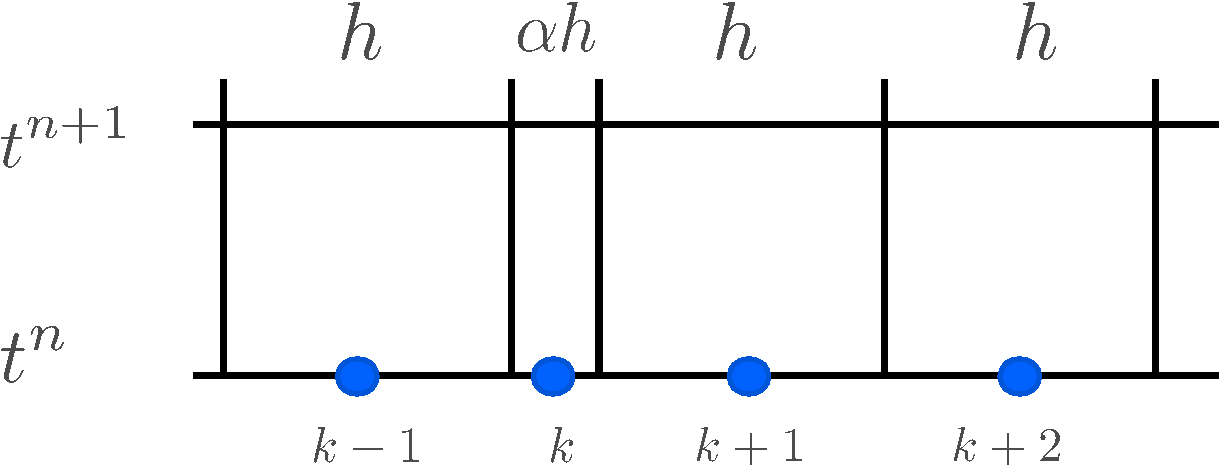
\includegraphics[height=1.3in]{figs/1dfig.pdf}
\caption{\sf Notation for model problem in one space dimension. The small
cell has size $\alpha h$ in a mesh with regular mesh width $h$.}
\label{fig:modelProblem1}
\end{center}
\end{figure}

To set the stage, notice that cell merging can
be rewritten as a postprocessing step.
To take one step to update a finite volume approximation to
$u_t + u_x = 0$ we do the following:
\begin{itemize}
\setlength\itemsep{.2in}
\item
{\bf Finite Volume Step}\\
Take the usual finite volume step with fixed, regular  $\Delta t$ on all cells 
including the small cell:
\begin{equation}
\bar{u}_j = u_j^n - \frac{\Delta t}{h_j} \; (f_{j+1/2} - f_{j-1/2} ), 
\quad \forall j.
\label{eqn:fvupdate}
\end{equation}

\item
{\bf {\em Temporarily} Create Merged Cell}\\
Temporarily create the {\em merged} cell $\overline{u_M}$ consisting of the small cell $u_j$ and one
or both of its neighbors so that it the merged cell is of sufficient
size (to be discussed later).  For simplicity here we will merge 
only with the neighbor on the right,
\begin{equation}
\widehat{u_M} =  \frac{ h_k \bar{u}_k + h_{k+1} \bar{u}_{k+1} } {h_k +
h_{k+1}} .
\label{eqn:mergestep}
\end{equation}

\item
{\bf Compute Merge Cell Gradient }\\
There are several ways to do this. 
\ref{sec:srdAlg}.
Two simple possibilities are 
\begin{equation}
\nabla \widehat{u_M} = \frac{\bar{u}_{k+2} - \bar{u}_{k-1}} {x_{k+2}-x_{k-1}}
\label{eqn:gradLim1}
\end{equation}
which does not use the merged cell,
or
\begin{equation}
\nabla \widehat{u_M} = \frac{\bar{u}_{k+2} - \widehat{u_{M}}} {x_{k+2}-x_{M}}
\label{eqn:gradLim2}
\end{equation}
which uses the merged cell, and $x_M$ is the centroid of the merged
cell.
The choice of gradient stencil will be studied later. 

%Other more accurate alternatives exist, not all of which are stable.
%It would be better to use smaller stencils, perhaps including $u_{k+1}$
%or $\overline{u_M}$ itself.

\item
{\bf Redistribute Merged State to Cells Comprising Merged cell }\\
Replace the provisional values computed in the cells comprising the
merged cell with the merged solution reconstructed to the cell
centroids:
\begin{equation}
\begin{split}
u_k^{n+1} &= \widehat{u_M} +  (x_k - x_M) \nabla \widehat{u_M}\\
u_{k+1}^{n+1} &= \widehat{u_M} +  (x_{k+1} - x_M) \nabla \widehat{u_M}
\end{split}
\end{equation}
\end{itemize}
This method is clearly linearity preserving if all gradients are
computed accurately enough to preserve a linear function.  
It is conservative since the mass of the merged cell equals the mass of
the two cells comprising it, and the linear function through the
centroid also has the same amount of total mass.

When written in one-step form instead of as a post-processing step, 
it is seen to be closely related to cell merging. 
In the first order case without gradient, the above gives
\begin{equation}
u_k^{n+1} = u_{k+1}^{n+1} = \widehat{u_M}^{n+1} 
\end{equation}
Pluging in the updates for $\widehat{u_M}$ we get
\begin{equation}
\widehat{u_M}^{n+1} = \widehat{u_M}^n - 
\frac{\Delta t}{h_k + h_{k+1}} (f_{k+3/2} - f_{k-1/2})
\end{equation}
Recognizing that $h_k+h_{k+1}$ is the merged cell volume makes this
clear.
By using a higher than linear polynomial and
including more neighbors in the
redistribution (on top of a more accurate scheme for the entire grid),
we have a path to higher order accuracy.
%By including gradients it provides a path to higher dimensions, possibly 
%overlapping neighborhoods. 

The choice of merging neighborhoods and gradients is what makes up the
specifics of SRD in two space dimensions. Furthermore, it can happen
that a cell has more than one neighborhood with
which it should merge. This is what often causes complications in cell
merging algorithms. In SRD, we will simply use all such values appropriately
weighted.

In the next section we present the SRD algorithm in two dimensions.
For simplicity we present the second order accurate version first.
The more general higher order extension is described in 
section \ref{sec:ho}.
Some theoretical results using one-dimensional model problems are in
section \ref{sec:theory}. 
Section \ref{sec:compResults} shows computational results for both smooth
problems and shocked flow for both linear advection and the Euler equations.  We conclude in section \ref{sec:conc}.


\section{The State Redistribution Algorithm}\label{sec:srdAlg}

We first describe the second order accurate version of the State
Redistribution Algorithm. 
This helps simplify the notation and make the
algorithm more intuitive.   
At several places there are choices
to make, and we discuss the alternatives and the reason behind our
choices.  

\subsection{The State Redistribution Algorithm}

To start, we define two quantities associated with each cell of the mesh:

\begin{itemize}
\item
{\bf Each cut cell finds adjacent cells to {\em temporarily} merge with.}

\vspace*{.1in}
For each cut cell in the mesh, find  one or more neighbors until the
volume of the temporarily merged cell is at least half the area of an uncut cell, i.e., 
\begin{equation} \label{eq:vmerge}
\sum_{(k,l) \in M_{i,j}} V_{k,l} \geq \frac{1}{2}\Delta x\Delta y,
\end{equation}
where $M_{i,j}$ denotes the set of cell indices that belong to merging neighborhood $(i,j)$.
We call this the 
{\em  merging neighborhood} or {\em merging tile}.  
A small cell can be merged with cells in the direction closest to the boundary normal (Figure \ref{fig:neighborhoods}, left), or with all cells that are at most e.g. one cell away, that is, cells located on the $3 \times 3$ tile centered at the small cell (Figure \ref{fig:neighborhoods}, right).
The larger the neighborhood the more diffusive the results, therefore we use the normal neighborhood everywhere possible.
There are instances where the normal neighborhood cannot be used, e.g., if a neighboring cell is also cut and the
merging neighborhood is not sufficiently large (Figure \ref{fig:normalneighborhood}).  In this case, we must merge with cells on the $3\times3$ tile (Figure \ref{fig:3x3neighborhood}), or, if that merging neighborhood is not large enough, with cells on the $5 \times 5$ tile.

\begin{figure}
    \centering
    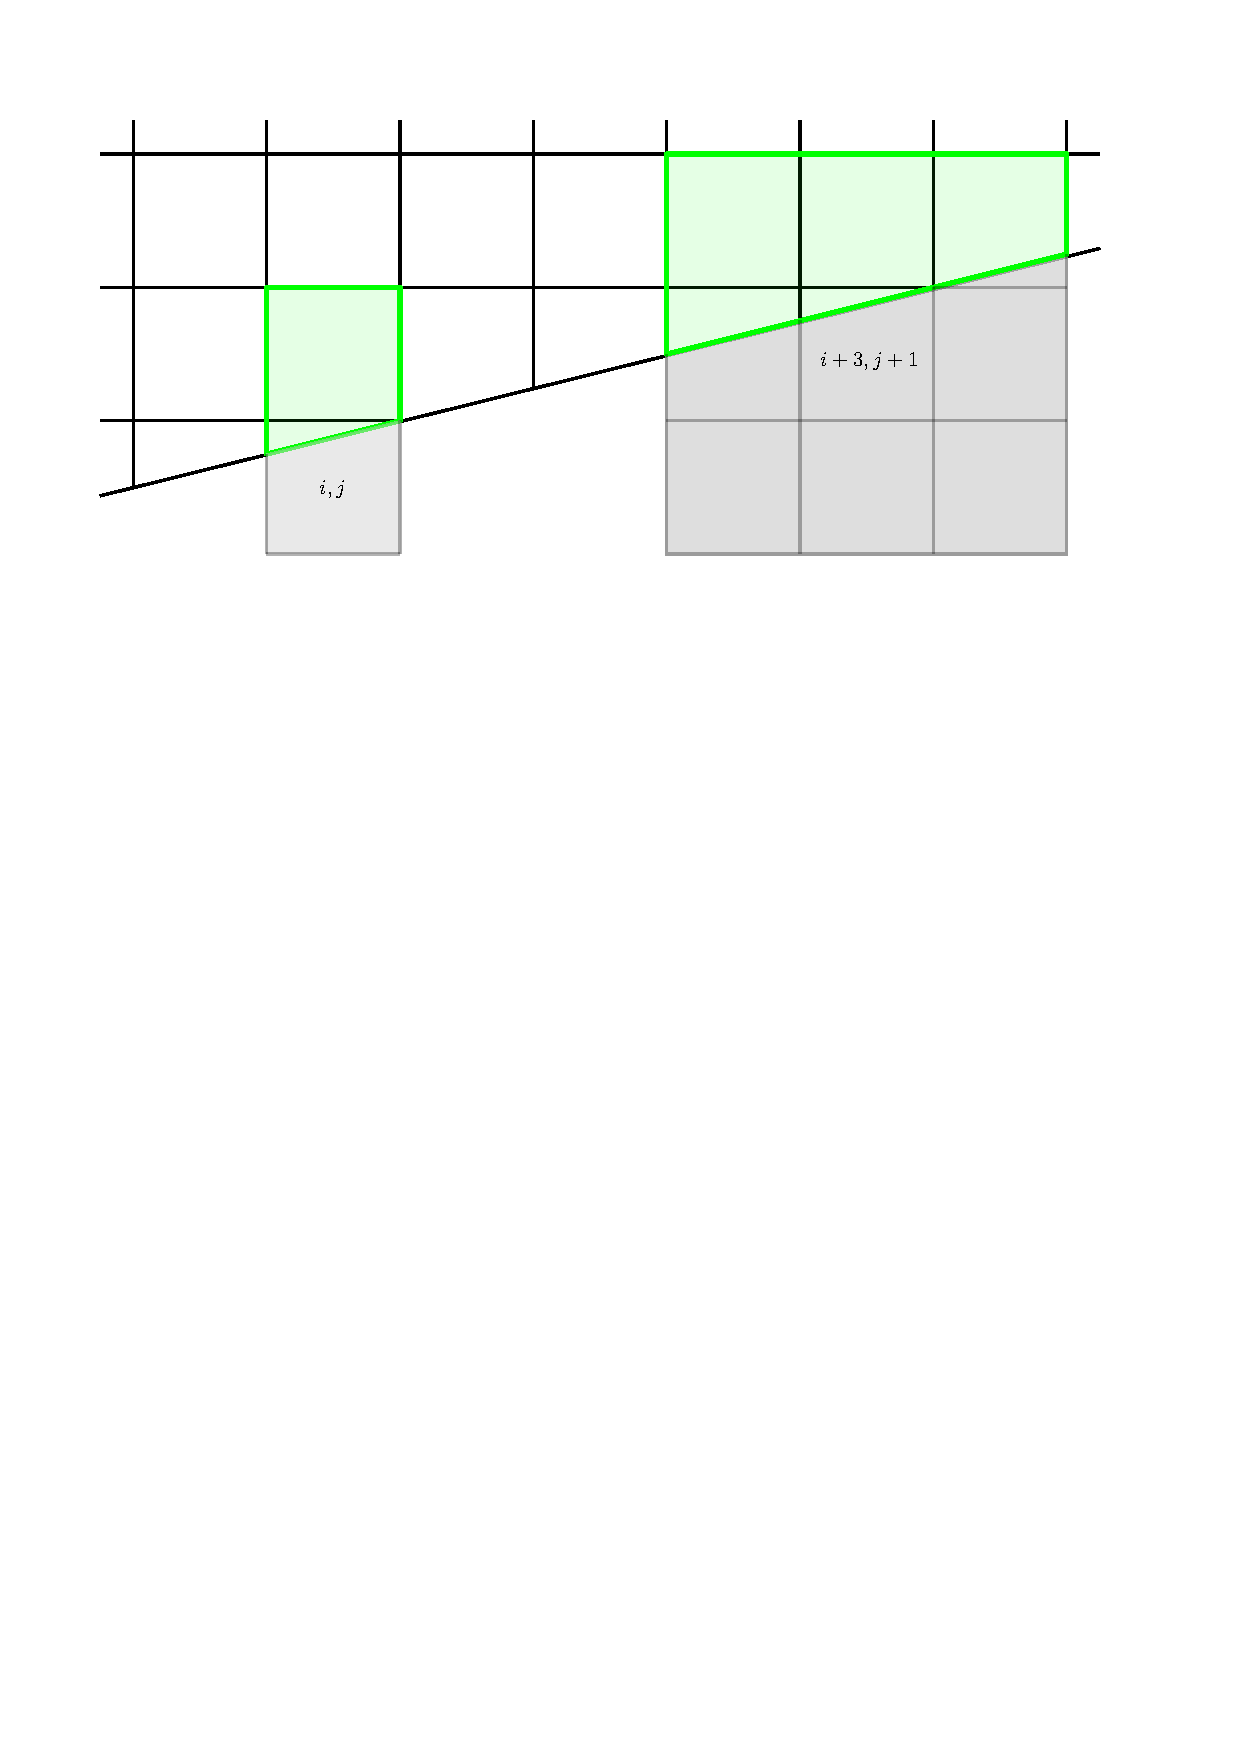
\includegraphics[width=0.5\linewidth]{figs/neighborhoods.pdf}
    \caption{\sf On the left, a small cell is merged with a cell in the direction 
    normal to  the wall.  On the right, a small cell is merged with neighbors that are at most one cell away, i.e., cells located in the $3\times3$ tile.}
    \label{fig:neighborhoods}
\end{figure}

\begin{figure}
	\subfloat[\sf Normal neighborhood (in red) for both small cells in the right corner.]{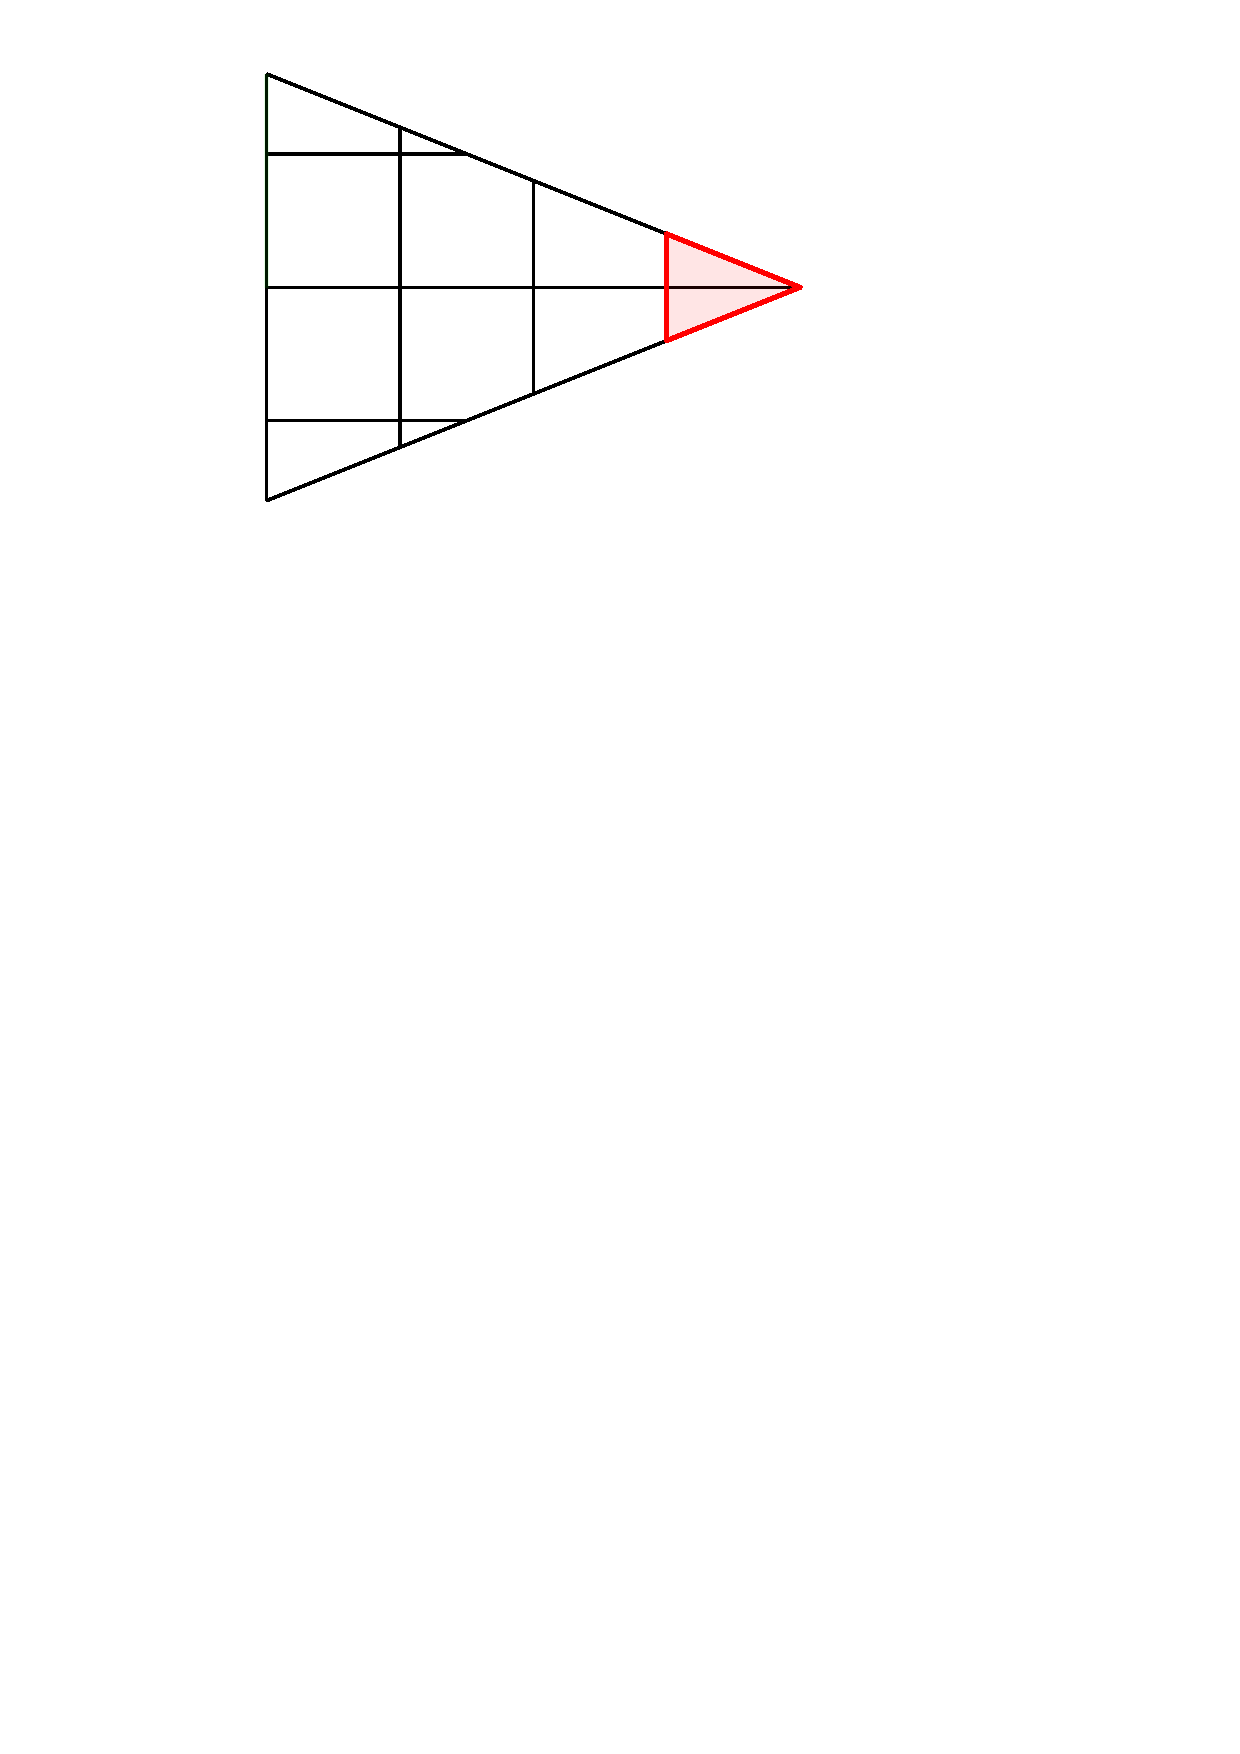
\includegraphics[width=.45\textwidth]{figs/normaldirection1.pdf} \label{fig:normalneighborhood}}
	\hfill
	\subfloat[$3\times 3$ merging neighborhood for both small cells in the right corner.]{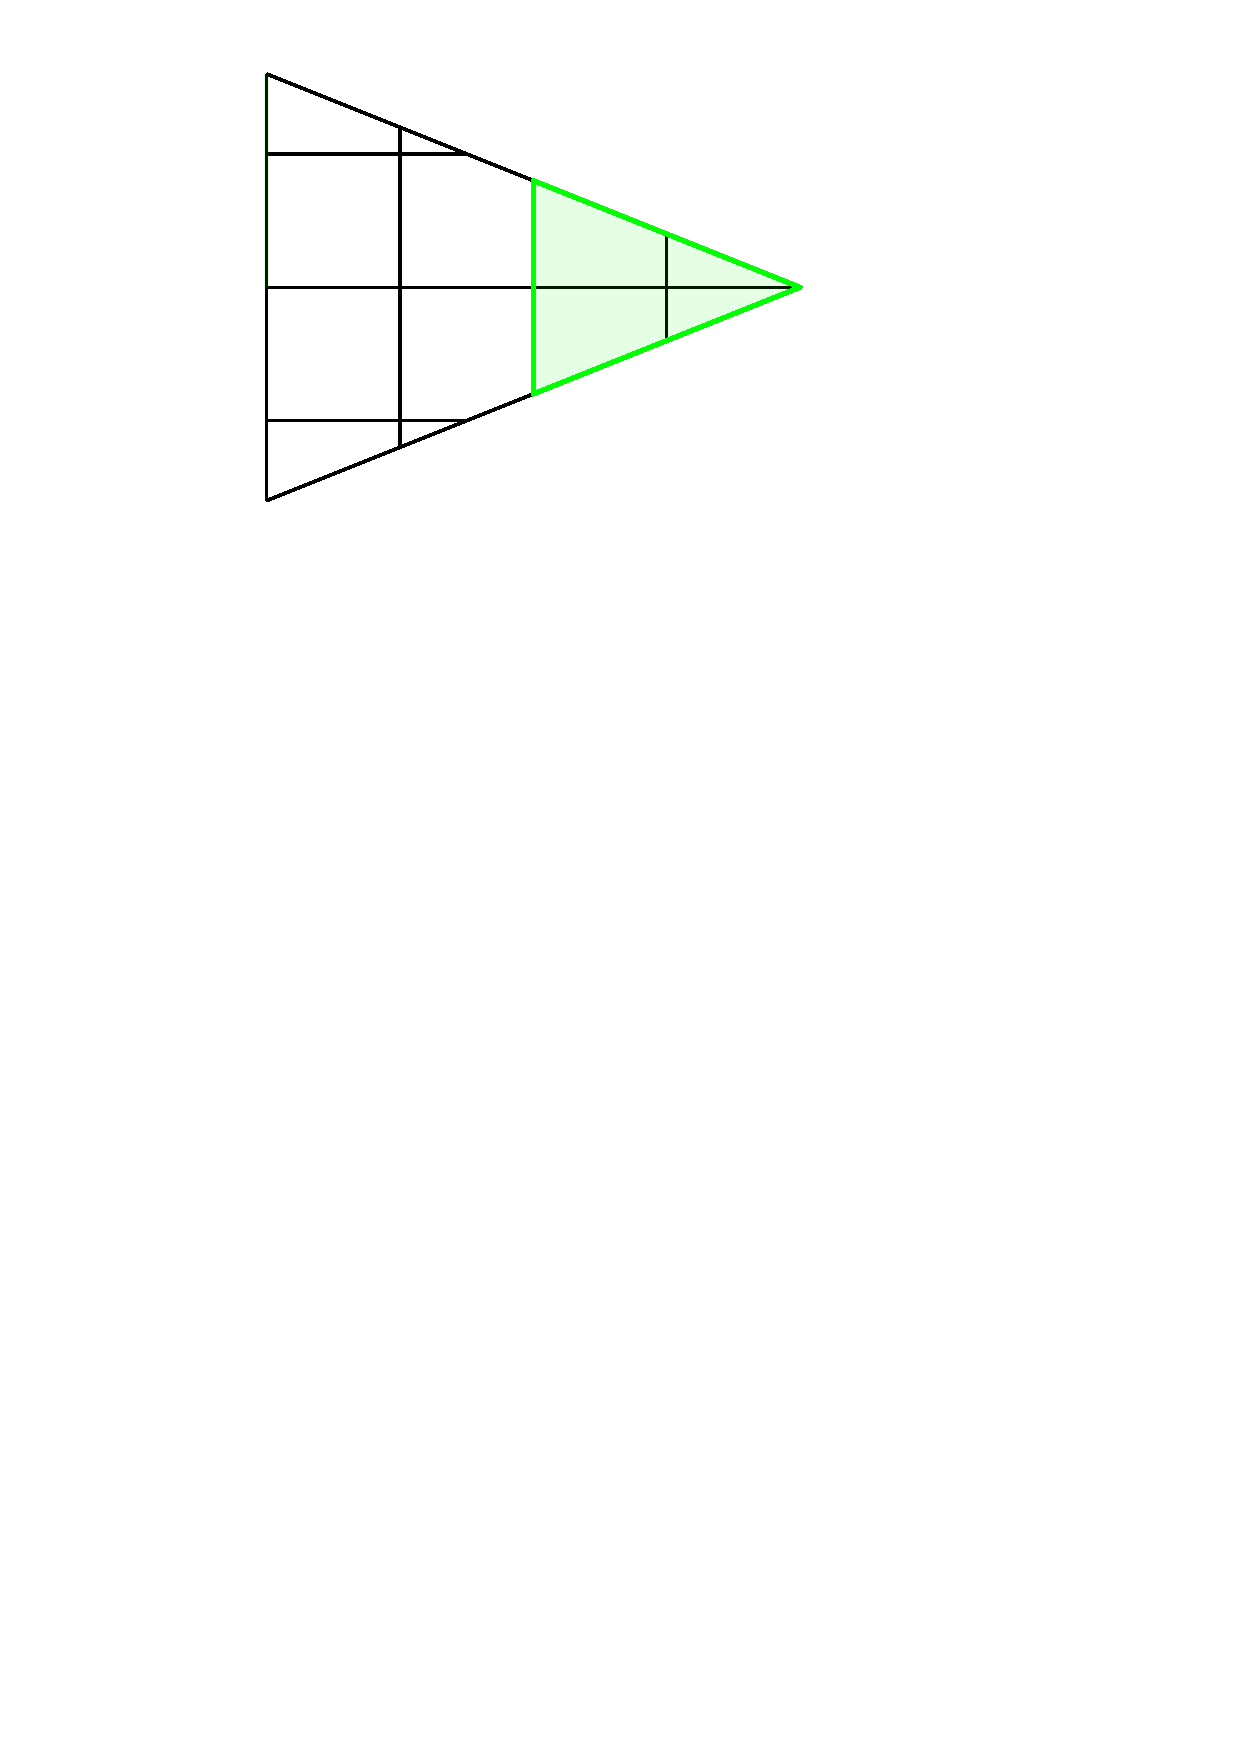
\includegraphics[width=.45\textwidth]{figs/normaldirection2.pdf} \label{fig:3x3neighborhood}}
	\caption{\sf Sometimes, the normal neighborhood is not large enough if a small cell merges with another small cell.  In this case, we use the $3\times 3$ tile, or $5\times5$ neighborhood until the volume constraint \eqref{eq:vmerge} is satisfied.}
\end{figure}
% If the neighboring cell 
% is also cut, it can happen that the
% merged cell is not sufficiently large (SHOW EXAMPLE?). 
% Next we try a 2 by 2
% neighborhood, including the original cut cell. Later we also show
% results using a 3 by 3 neighborhoods. However the larger the
% neighborhood the more diffusive the results.

% Note that this does not have the difficulty of cell merging, since 
% overlapping neighborhoods are allowed. 

\item
{\bf Each cell counts how many neighborhoods it is a part of.}

\vspace*{.1in}
A full cell is its own merging neighborhood, since it has sufficient
volume all by itself. However, we will still refer to all cells as having a
merging neighborhood for ease of presentation.  In figure \ref{fig:overlappingneighs}, we provide an example cut cell mesh with all merging neighborhoods plotted.  We also display the number of overlapping neighborhoods on a cell, this is the neighborhood {\em count} for each cell.
\begin{figure}
	\subfloat[]{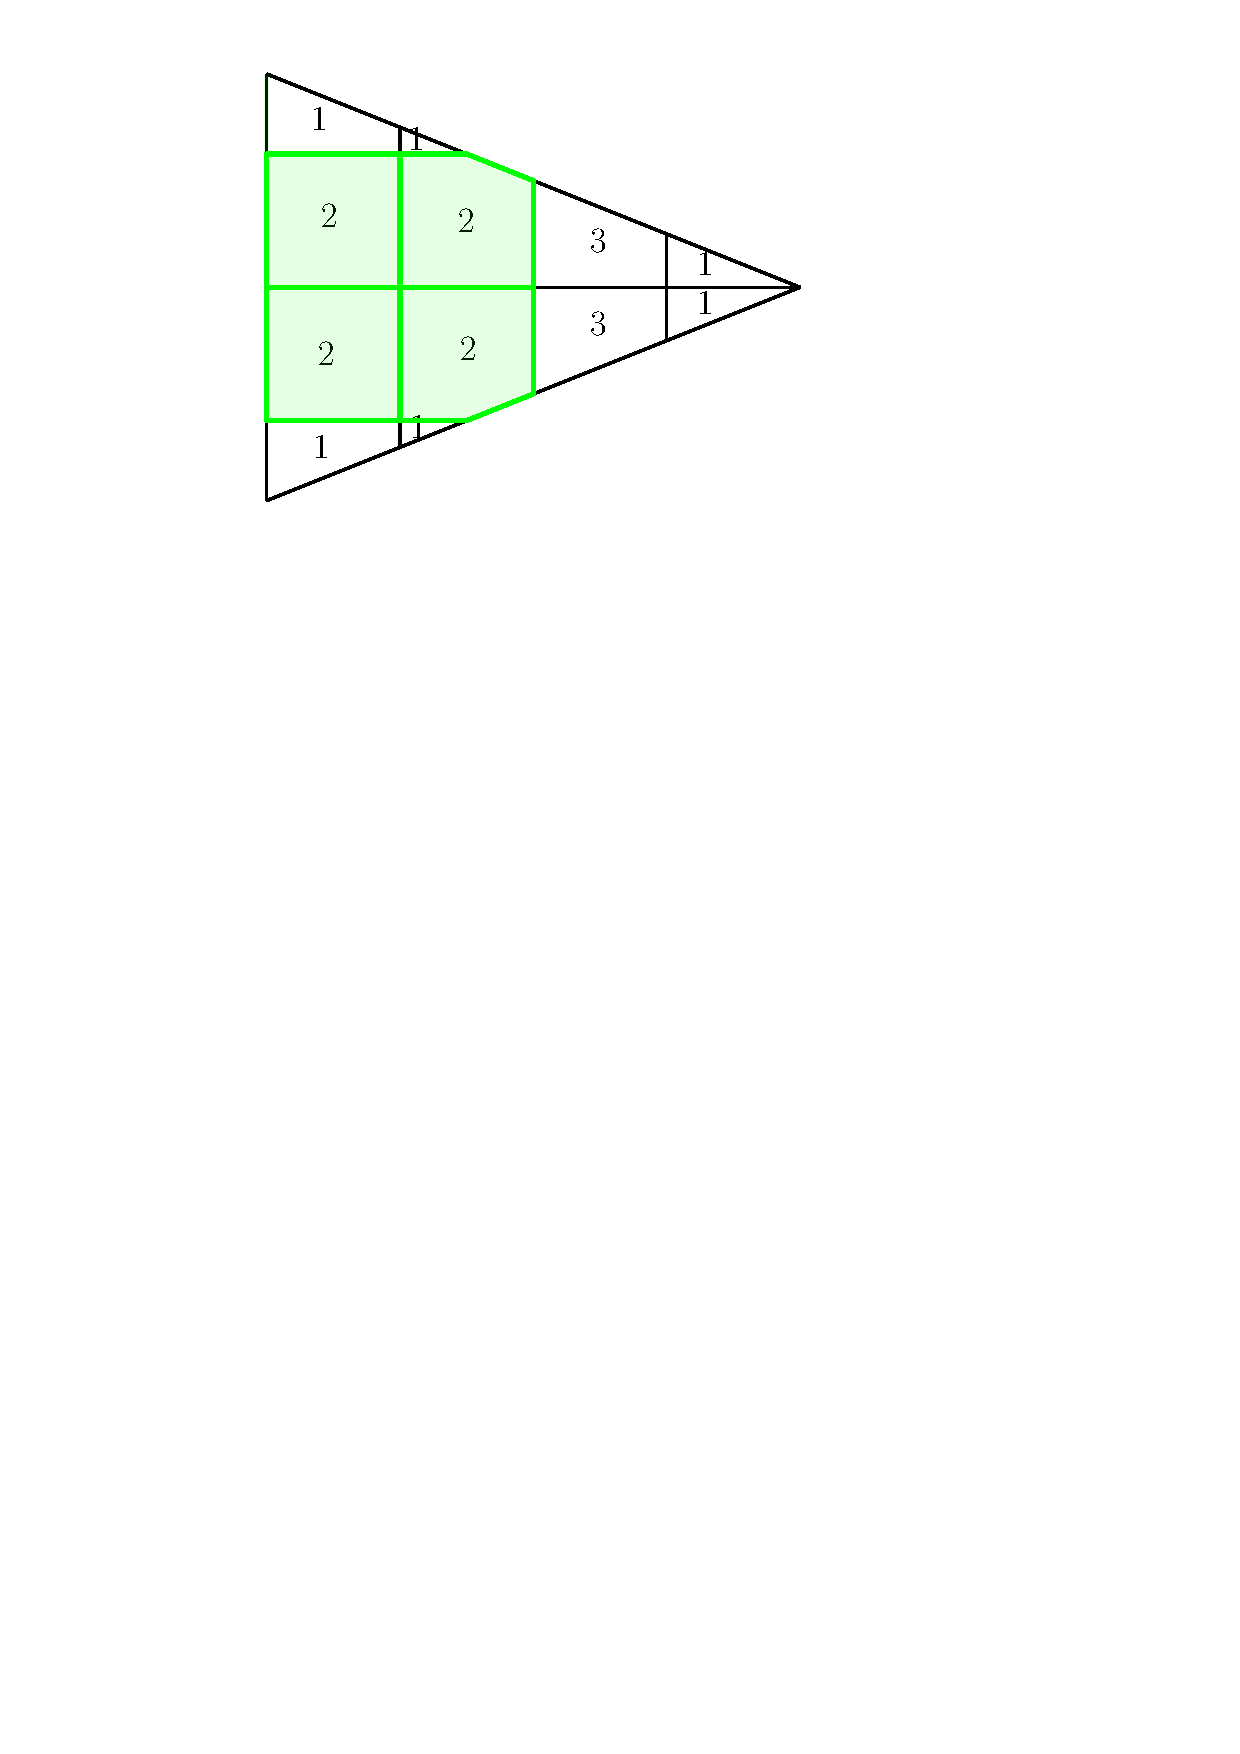
\includegraphics[width=.24\textwidth]{figs/numoverlaps1.pdf} \label{fig:numoverlaps1}}
	\hfill
	\subfloat[]{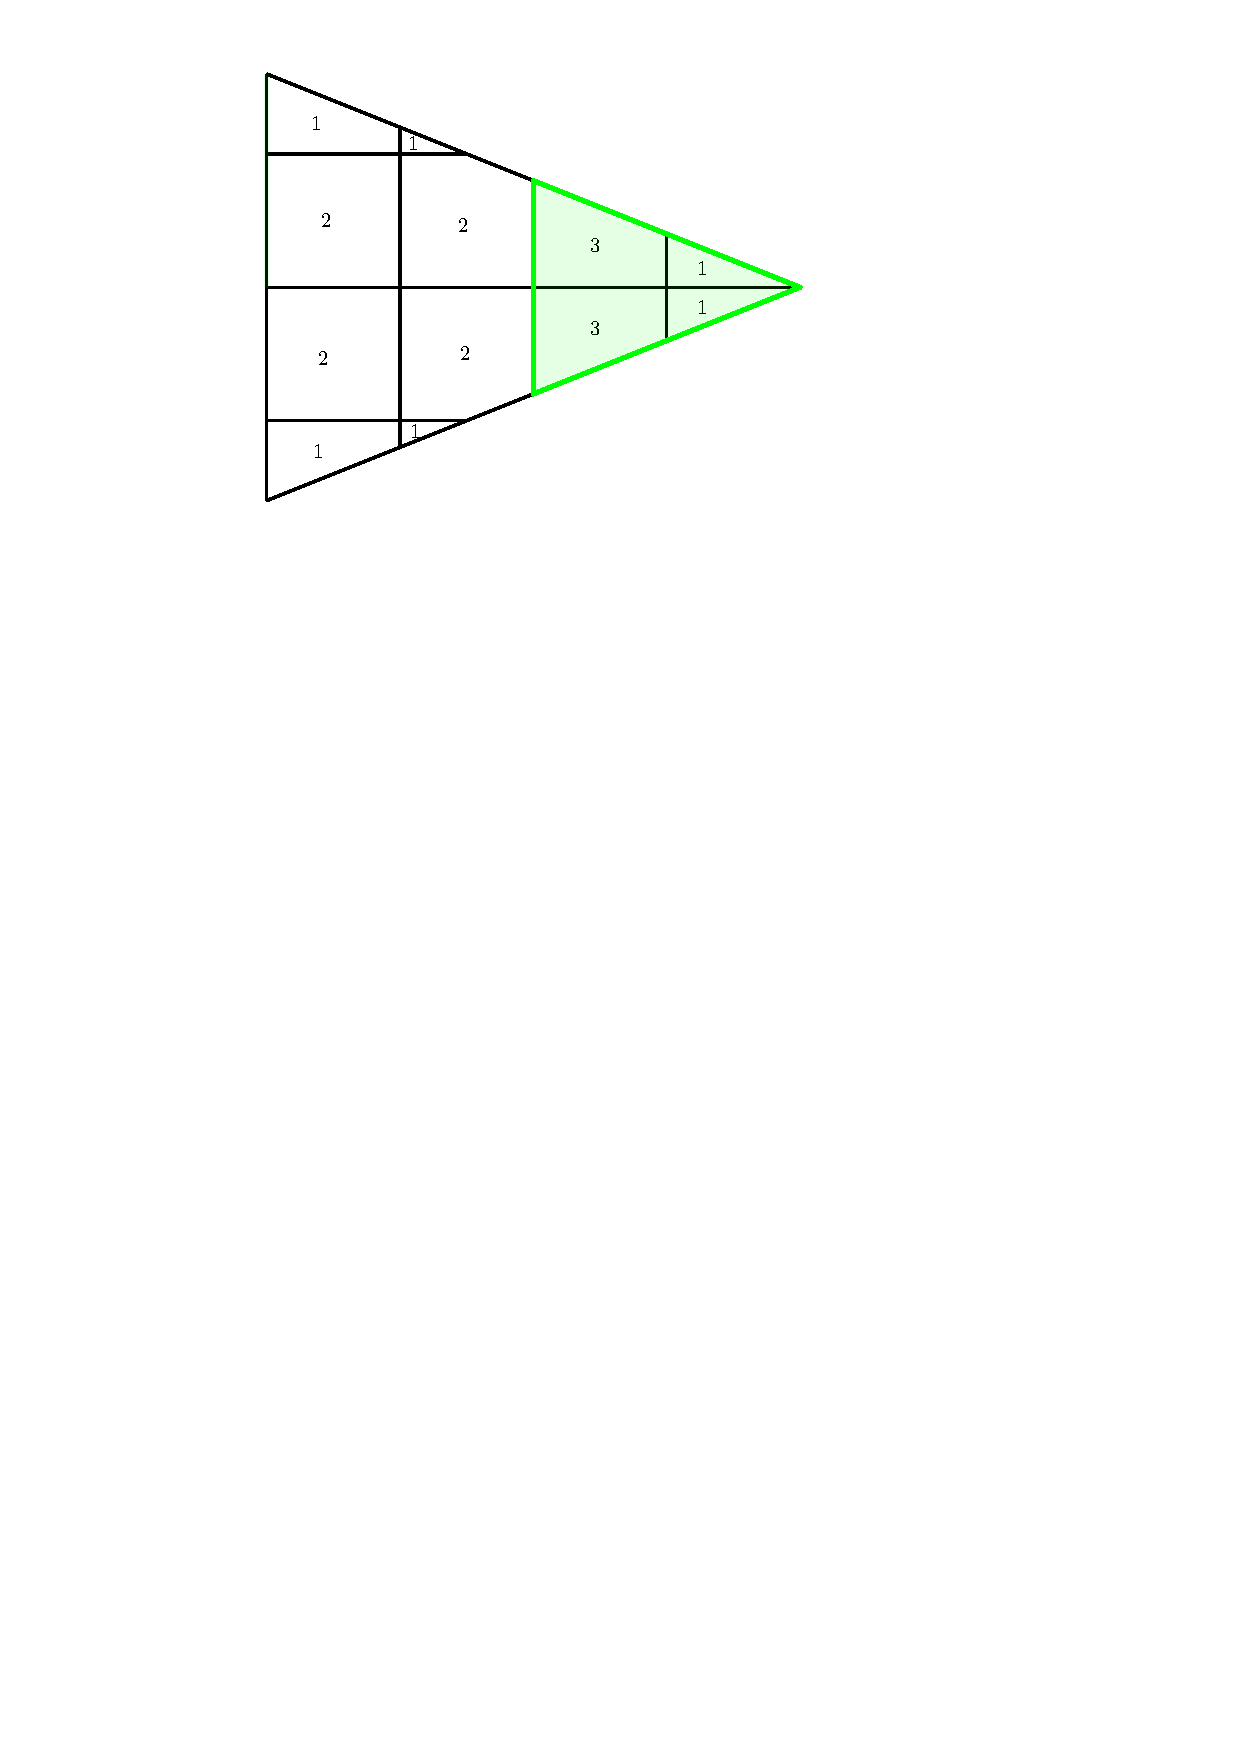
\includegraphics[width=.24\textwidth]{figs/numoverlaps5.pdf} \label{fig:numoverlaps4}}
	\hfill
	\subfloat[]{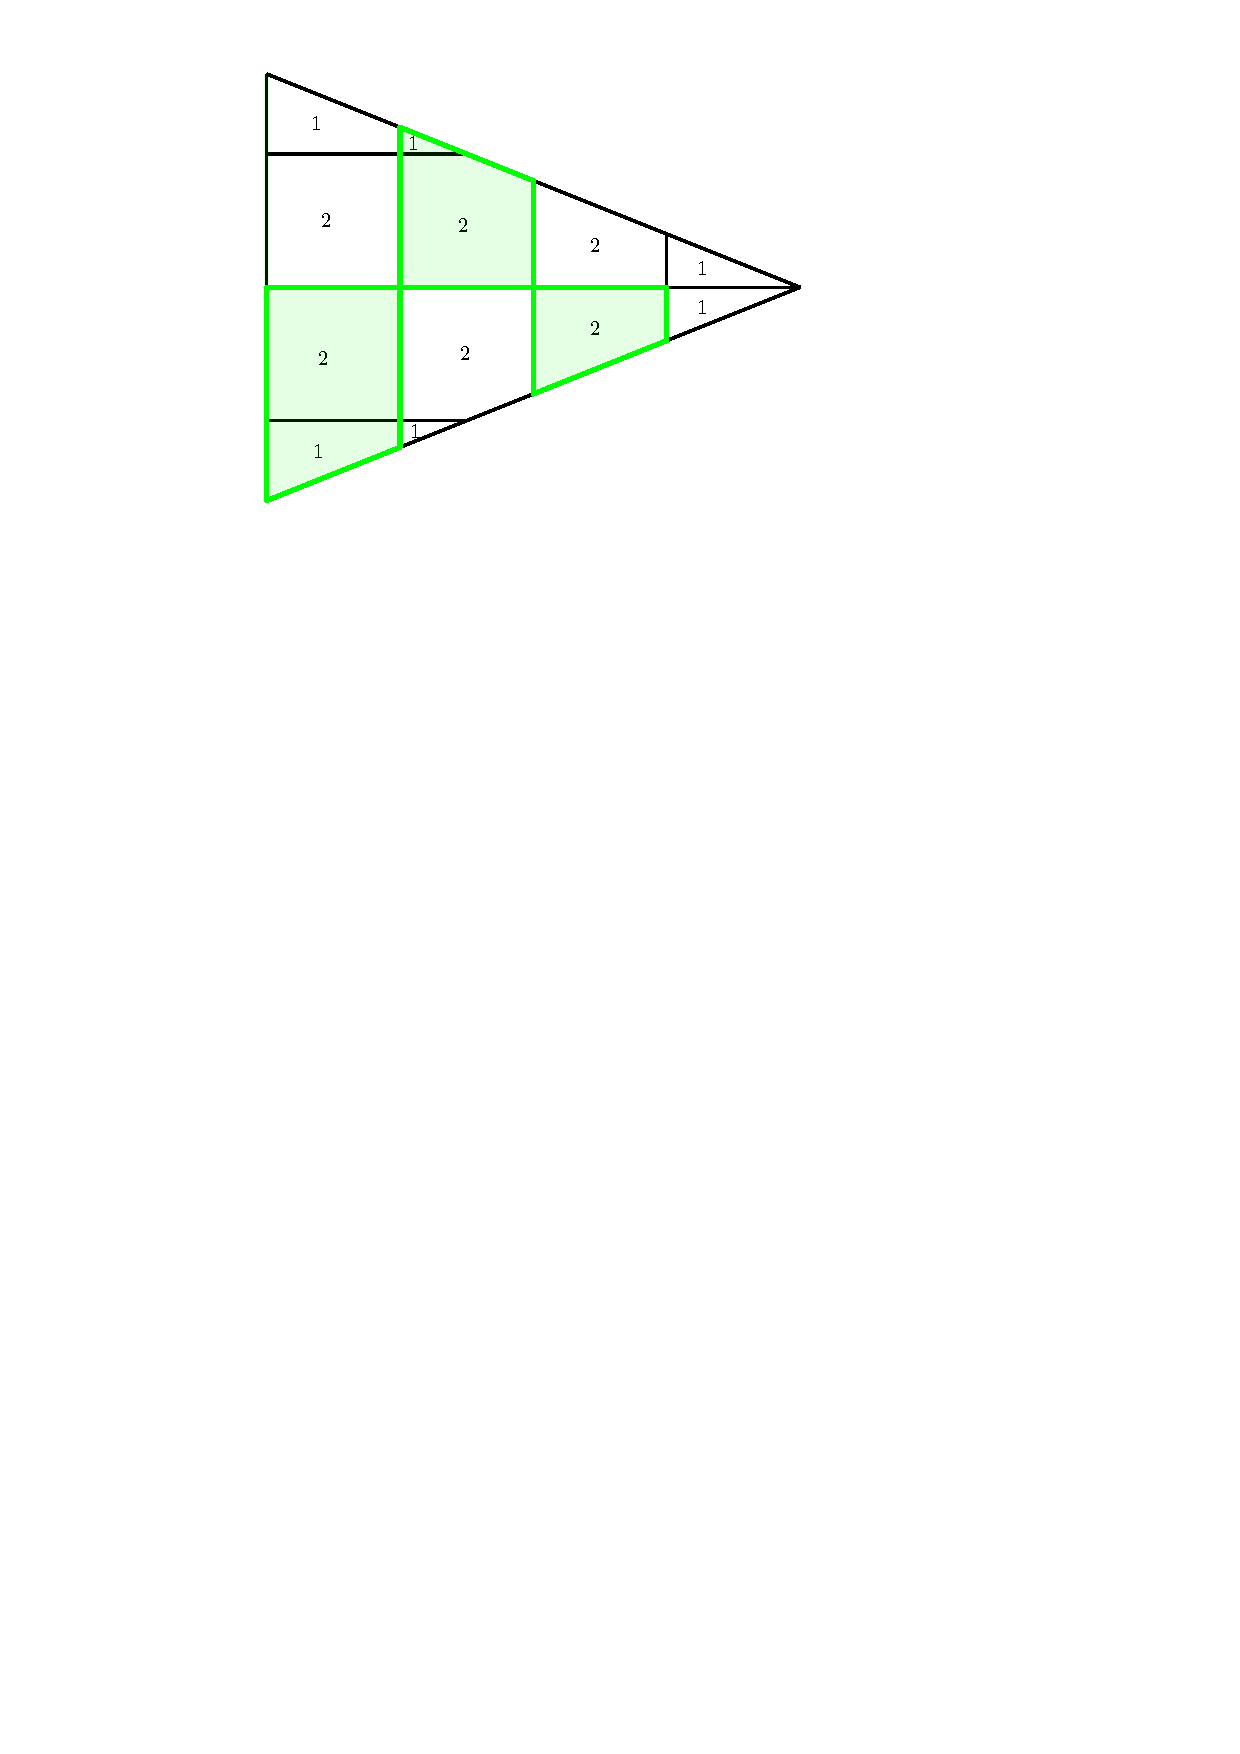
\includegraphics[width=.24\textwidth]{figs/numoverlaps2.pdf} \label{fig:numoverlaps2}}
    \hfill
	\subfloat[]{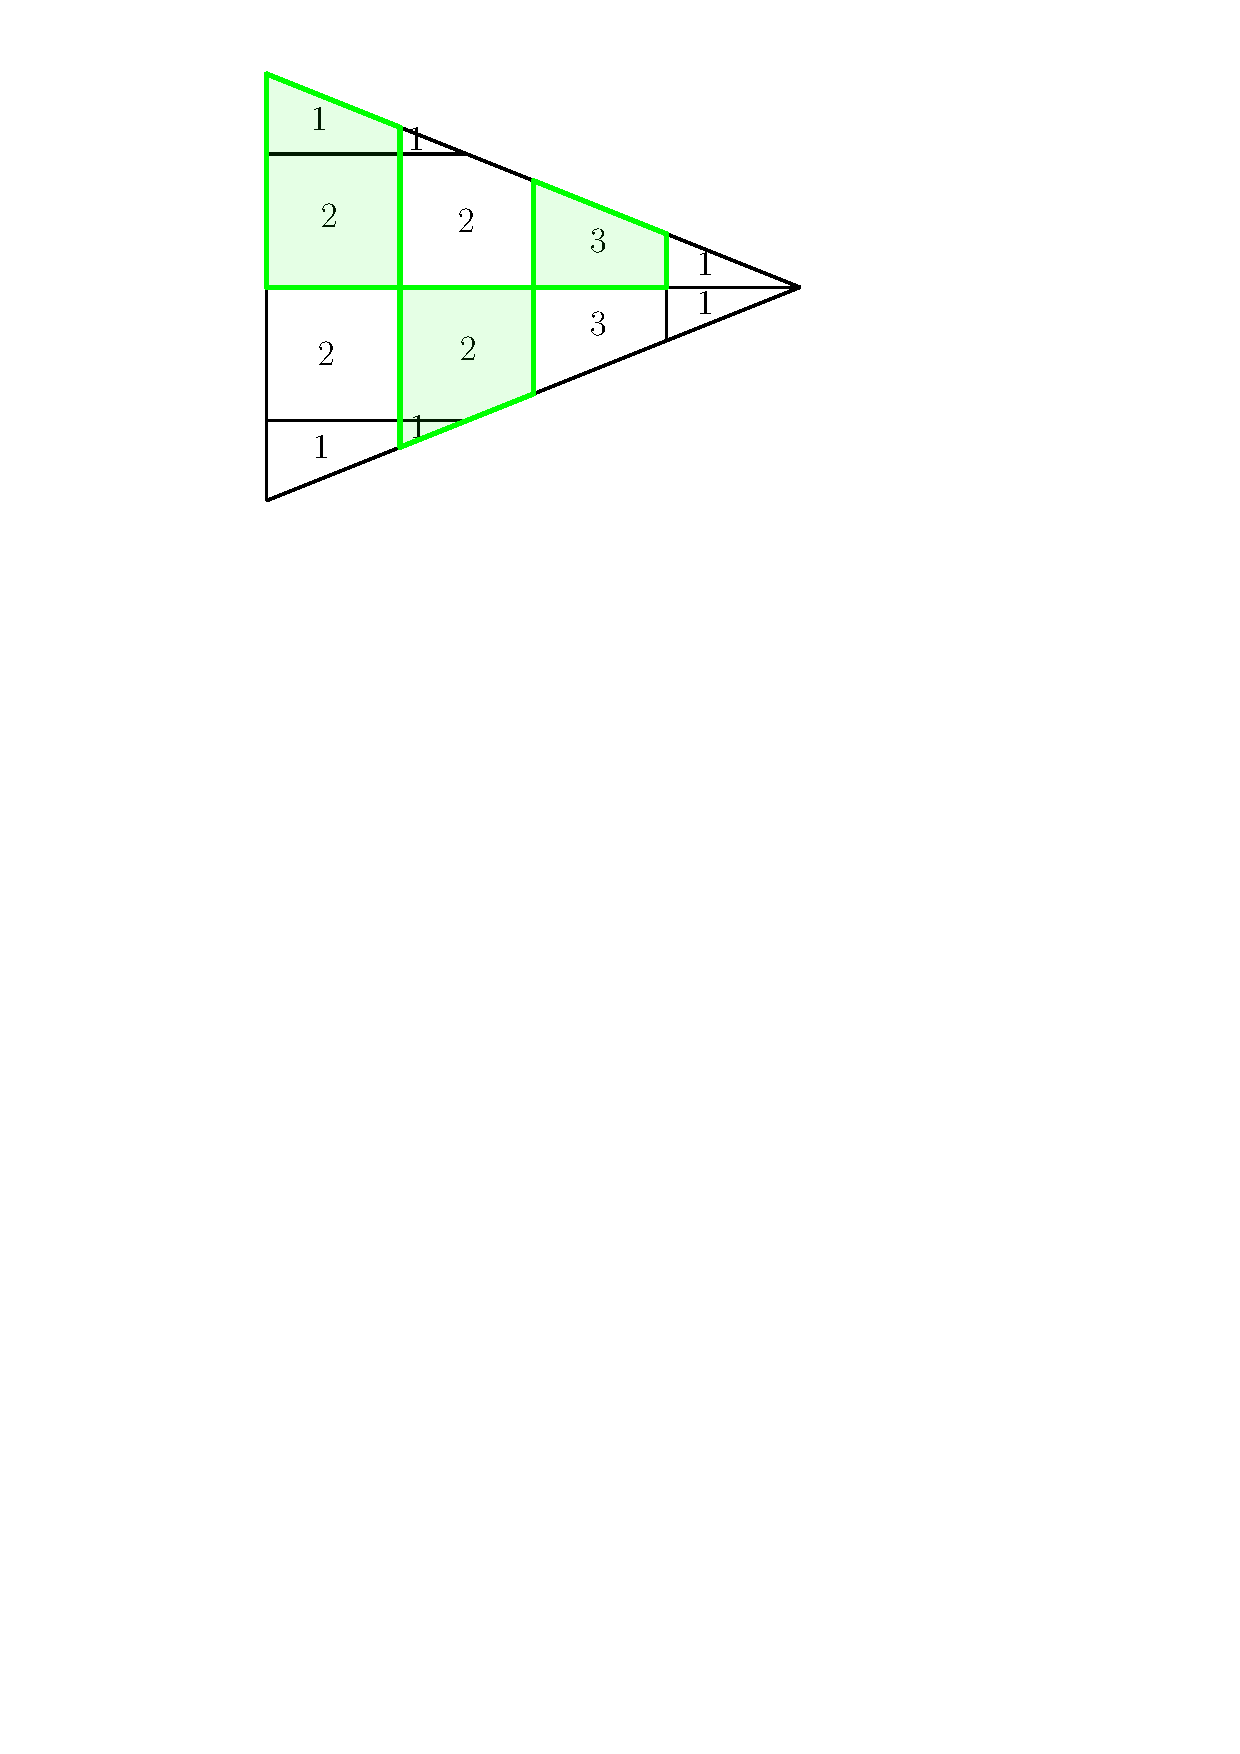
\includegraphics[width=.24\textwidth]{figs/numoverlaps3.pdf} \label{fig:numoverlaps3}}
	\caption{\sf All merging neighborhoods on an example cut cell mesh (in green).  We display the number of overlapping merging neighborhoods on each cell. Note, in figure \ref{fig:numoverlaps4}, there are two merging neighborhoods that occupy the same location, one per small cell in the right corner.} \label{fig:overlappingneighs}
\end{figure}
Note that a full cell
can be part of two or more merging tiles if it is placed next to 
several tiny cut cells. An example is shown in
figure \ref{fig:2nborTile}. The cells in green are part of two
neighborhoods, and those in red are part of three.   
 Most full
cells are only members of their own tile and will have a count of one.
Only cells within a narrow band of the cut cells will have a count
larger than one.


\end{itemize}



% \begin{figure}[h!]
% \begin{center}
% 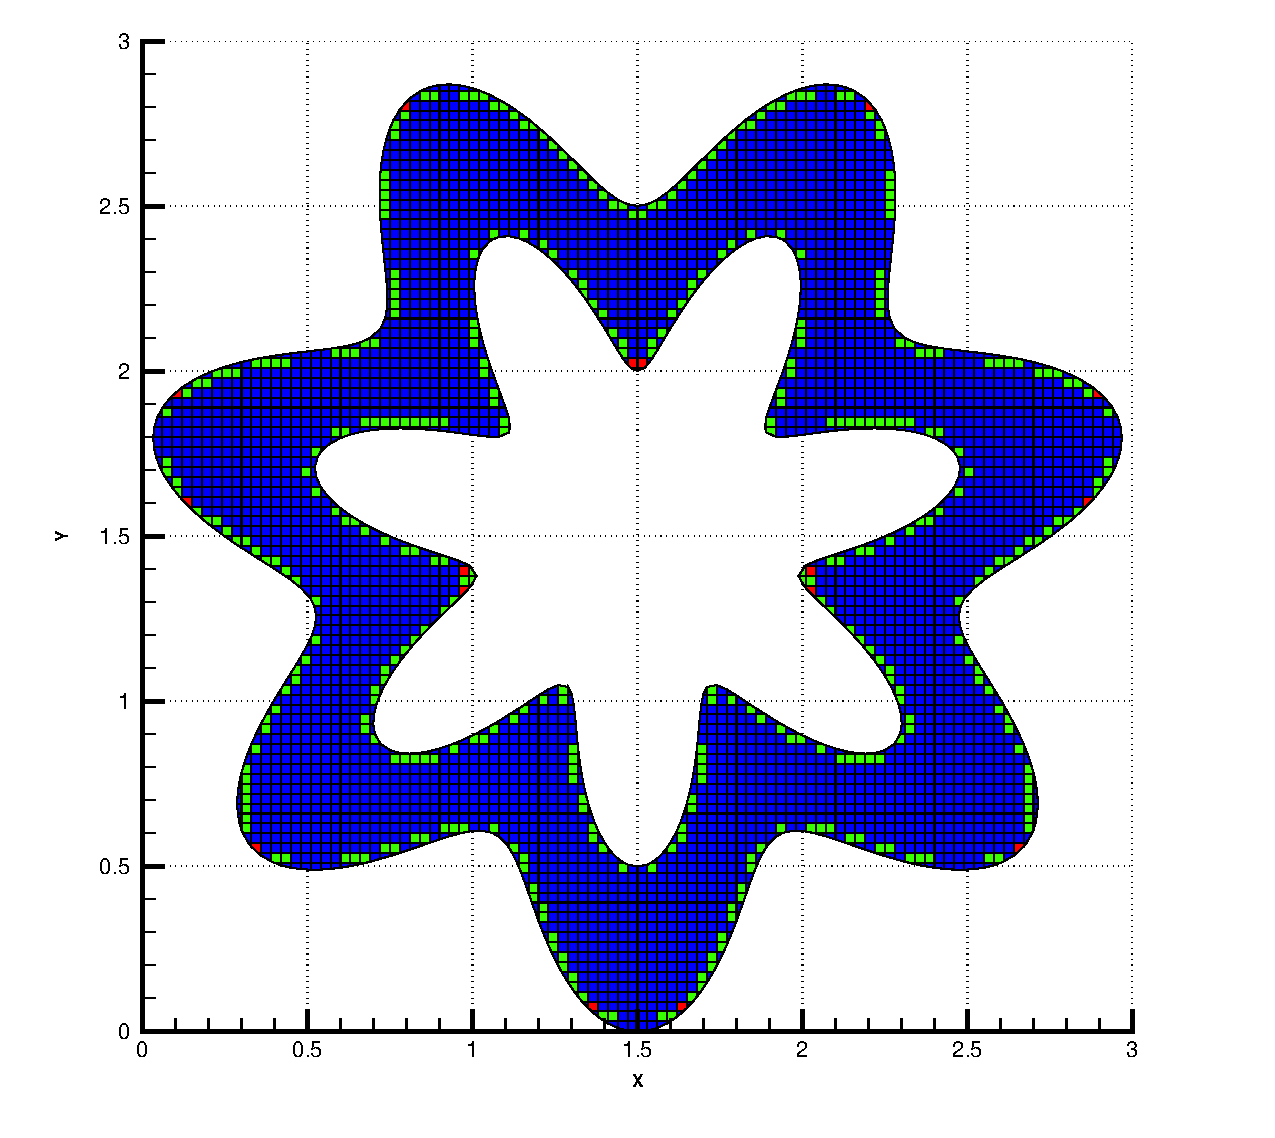
\includegraphics[width=4.5in]{figs/waveynumhoods.eps}
% \caption{\sf Domain from example XX.  Figure shows how many
% neighborhoods each cell belongs to: 
% one (white), two (blue), or three (red).
% The full example is shown in section \ref{sec:compResults}.}
% \label{fig:2nborTile}
% \end{center}
% \end{figure}

The two steps above can be part of a preprocessing step, since they do not
depend on the computed solution. For moving geometry however they would
be done at each step.
Using the merging tiles and the cell counts, the state redistribution
algorithm after one time step or stage is as follows:

%\begin{enumerate}[label=Step \arabic*:,leftmargin=2\parindent]
\begin{enumerate}
\item
{\bf Compute the volume-weighted and count-weighted solution for all
merged tiles.}   

\vspace*{.1in}
The contribution of each cell is divided by the number of neighborhoods 
it is part of (i.e. its count). The notation in this section refers
to cut cell $i,j$, with solution $U_{i,j}$ and volume
$V_{i,j}$. 
The provisionally updated solution before the
stabilization algorithm is applied is $\widehat{U}_{i,j}$.
There will now be many temporary merging neighborhoods which 
we denote as $\widehat{Q}_{i,j}$. 
Let $M_{i,j}$ denote the set of cell indices in the cell $(i,j)$ merging
neighborhood.  Then
\begin{equation}
\label{tiledef}
\widehat{Q}_{i,j} =  \frac{1}{{\widehat V}_{i,j}} \, \sum_{k \in M_i} \,  
\frac{V_k}{N_k}  \,\,  \widehat{U}_k
\end{equation}
where the volume ${\widehat V}_{i,j}$ is the merging tile volume similarly weighted,
\begin{equation}
\label{voldef}
{\widehat V}_{i,j} =  \sum_{k \in M_i } \,  \frac{V_k}{N_k}  .
\end{equation}

In other words, the contributions from each cell are weighted by the
number of neighborhoods they contribute to.
In the above equations, $k$ is  a multi-index ranging over the neighbors 
of cell $i,j$ included in its merging tile.
Note that most full cells will have ${\widehat V}_{i,j} = V_{i,j}$, 
and $\widehat{Q}_{i,j}  = \widehat{U}_{i,j}$.





\item
{\bf Compute a (limited) gradient for each merging
tile.}

\vspace*{.1in}
For cut cells, a least squares procedure  similar to the one used for
the finite volume update is an obvious choice. However instead of using the
solution $U_{i,j}$ on the Cartesian mesh at time $t_n$,
the merging neighborhood solution  $\widehat{Q}_{i,j}$ is used. It is important
to note that the centroid of the merging neighborhood is \textit{not} the centroid of cell ${i,j}$ (figure \ref{fig:centroids}).
\begin{figure}
    \centering
    \subfloat[]{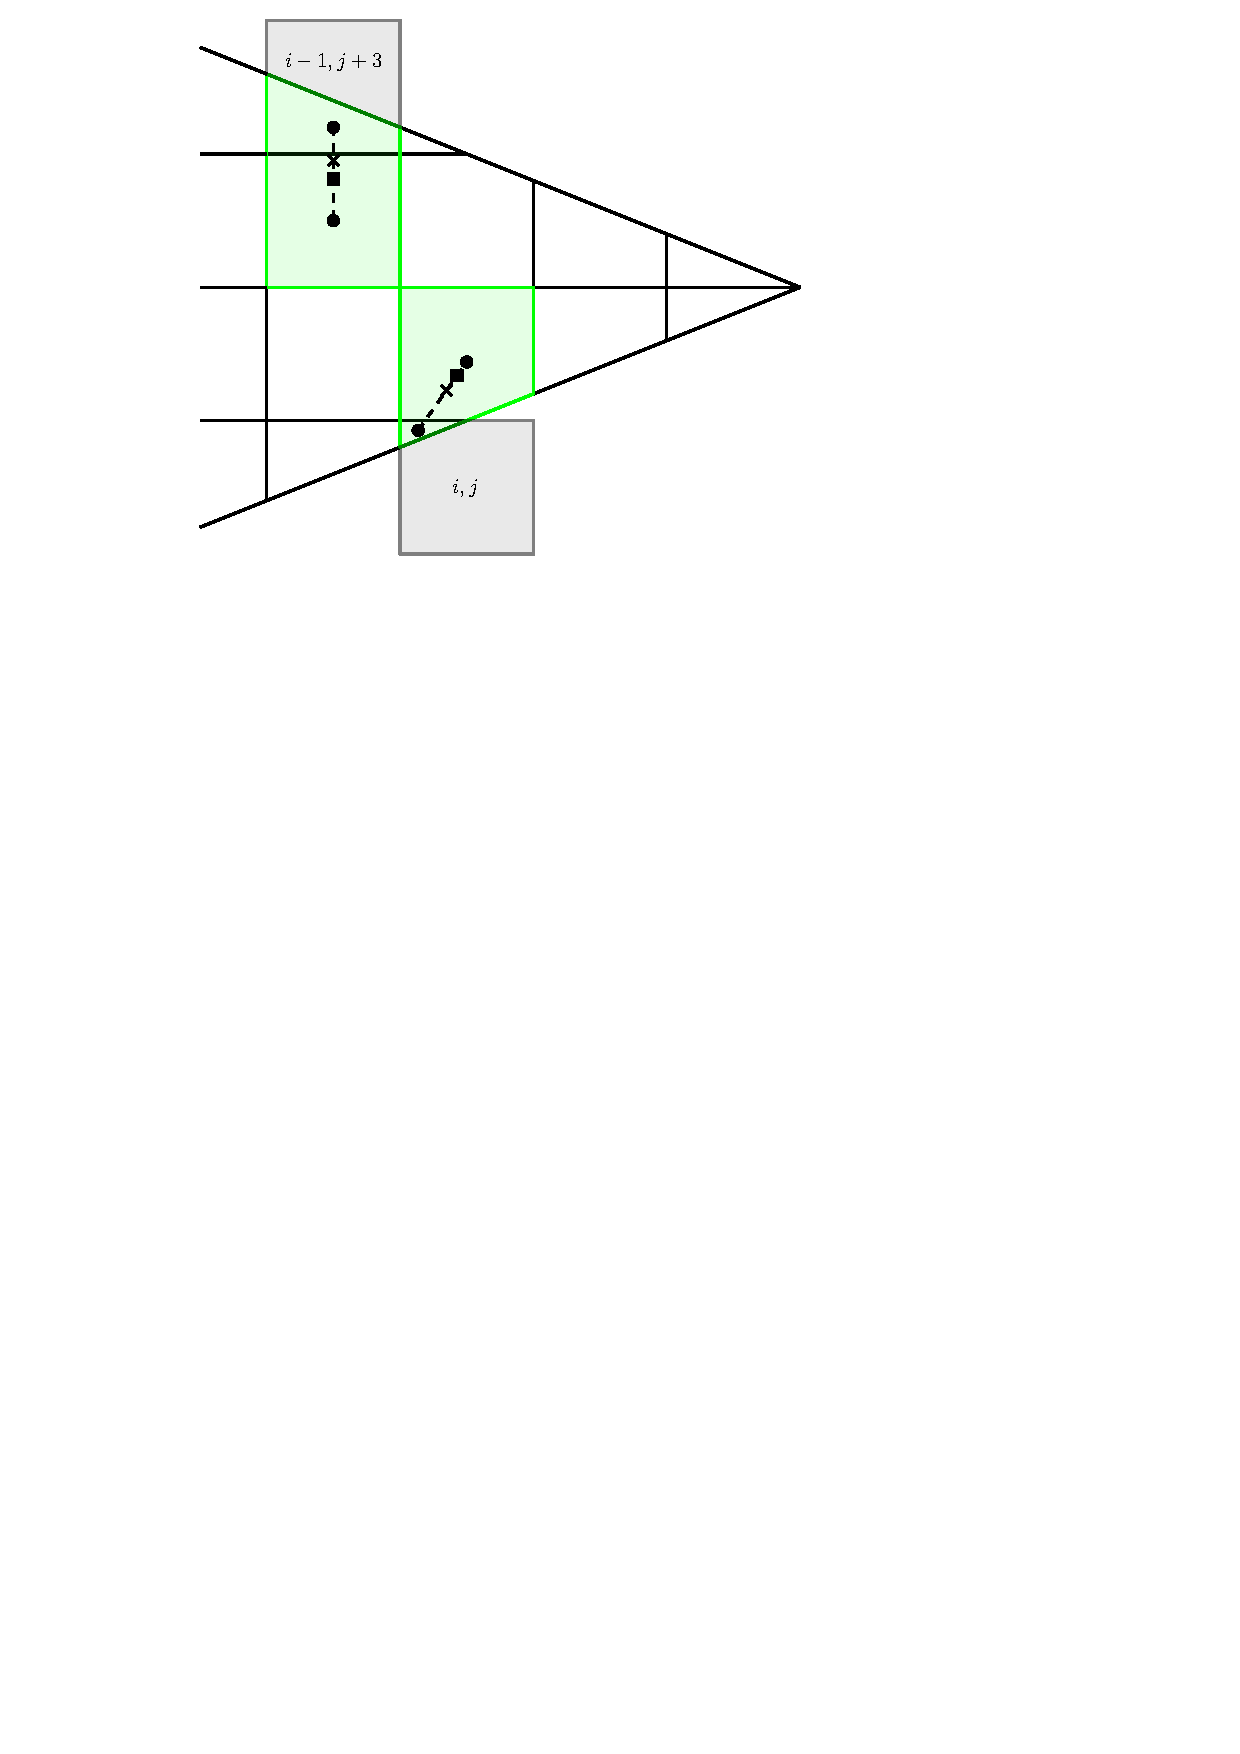
\includegraphics[width=0.45\linewidth]{figs/centroids3.pdf}} \hfill
    \subfloat[]{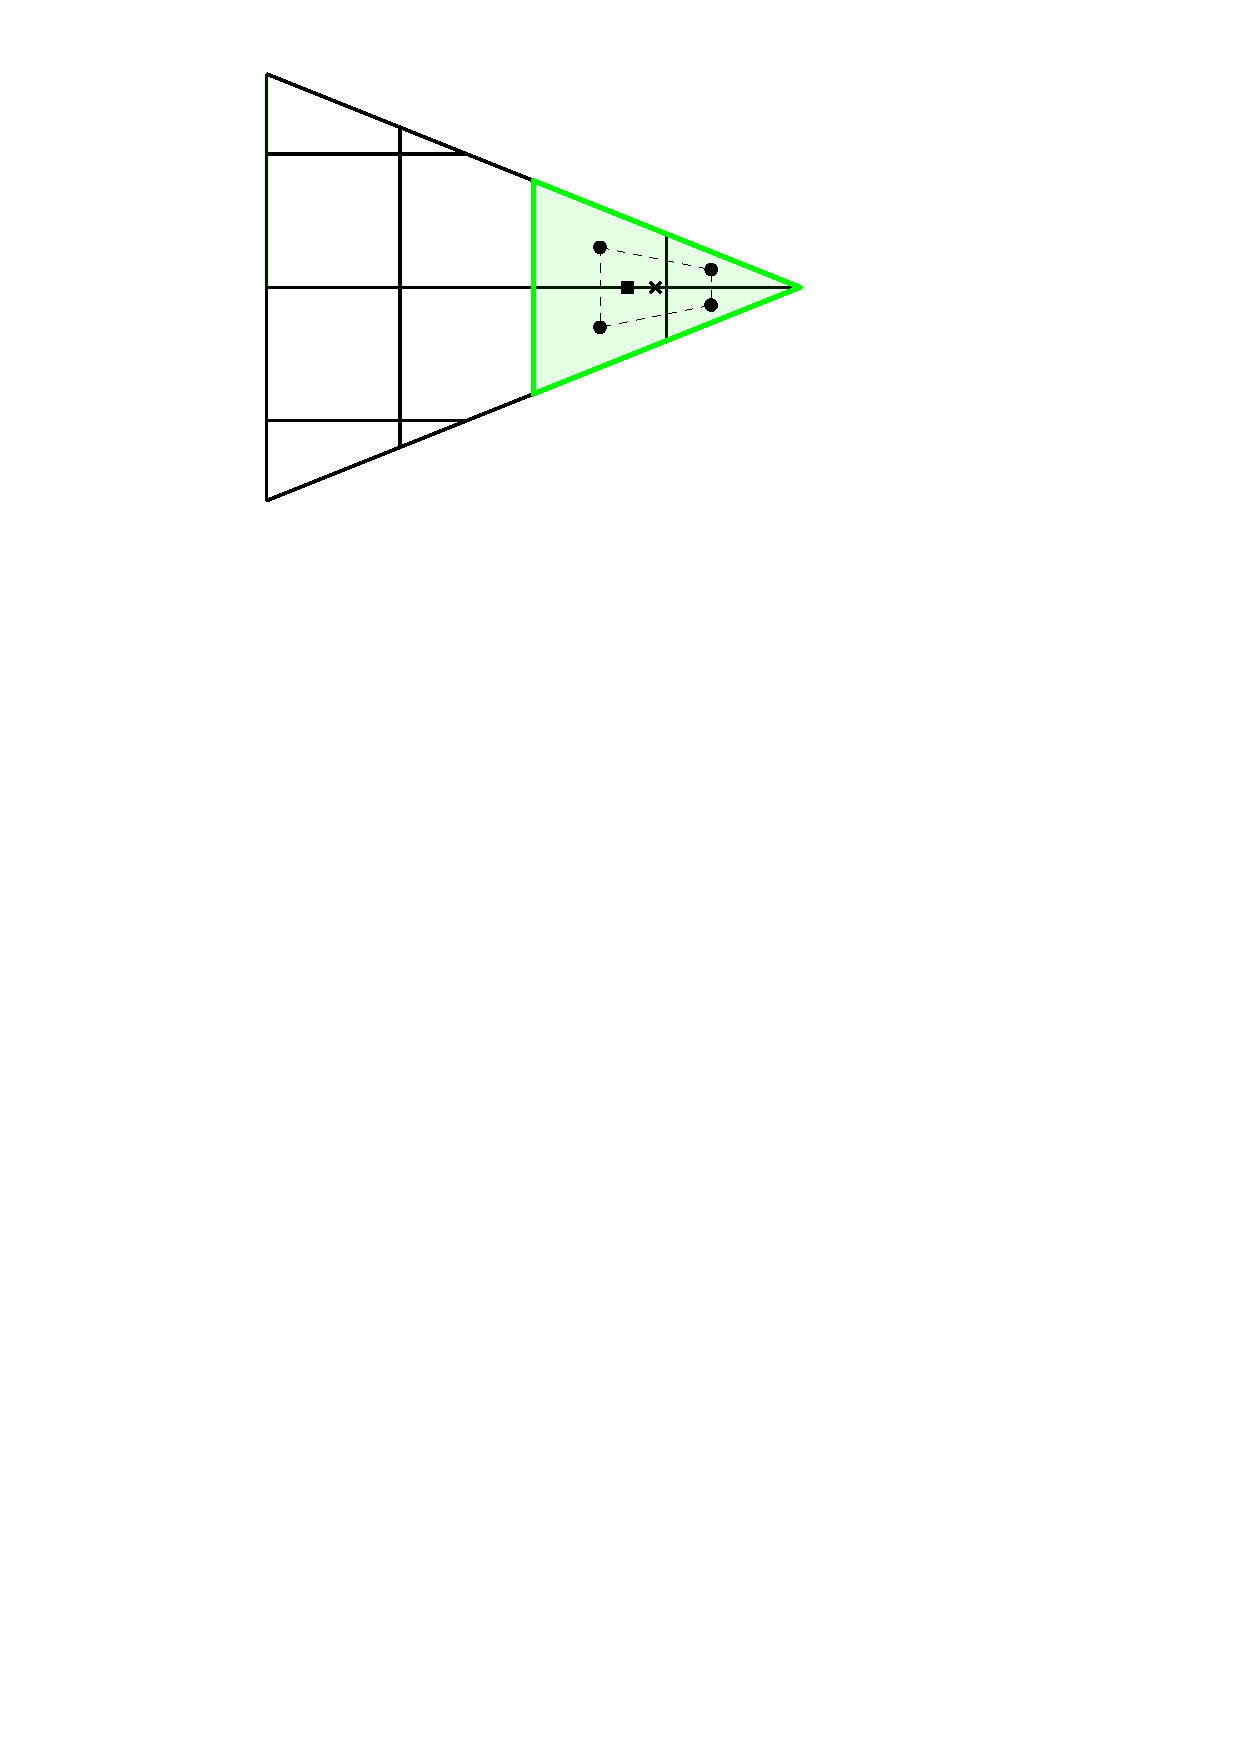
\includegraphics[width=0.45\linewidth]{figs/centroids4.pdf}}
    \caption{\sf The centroids of the Cartesian and cut cells are indicated with a solid circle ($\bullet$).  The centroids and weighted centroids of the merging neighborhoods are indicated with a square ($\blacksquare$) and a cross ($\times$), respectively. Note that the centroids and weighted centroid of the cut cell neighborhoods do not necessarily coincide.}
    \label{fig:centroids}
\end{figure}
The reconstruction neighborhood for $i,j$ is initialized to the $3 \times 3$ tile centered on $i,j$.
With this choice, it could happen that the centroids are too close to each other to compute a gradient in the normal direction (figure \ref{fig:tooclose}). If the weighted centroids are not at least $0.5\,\Delta x$  and $0.5\,\Delta y$ apart in the $x$ or $y$ direction then we increase the stencil size for the gradient computation.  For example, if the weighted centroids are too close in the $x$ direction, but not the $y$ direction, then the $5\times 3$ tile is used as the reconstruction neighborhood.  Similarly, if the weighted centroids are too close in the $y$ direction, but not the $x$ direction, then the $3\times 5$ tile is used as the reconstruction neighborhood.  The neighborhood size is increased until the distance constraint is satisfied in both directions.  In figure \ref{fig:tooclose}, the appropriate reconstruction neighborhood is $3\times 5$ reconstruction tile.
% The same neighborhood that is used for computing the gradient can be used to limit the gradient to prevent overshoots. The centroid is computed using the same weighting by number of neighborhoods as when the volume was computed. (IS THIS TRUE AND IS IT NECESSARY) NEED DISCUSSION OF NOT A REAL CENTROID
% For most full cells with a count of one, the normal gradient computation as done in the finite volume update will suffice.

\begin{figure}
    \centering
    \subfloat[]{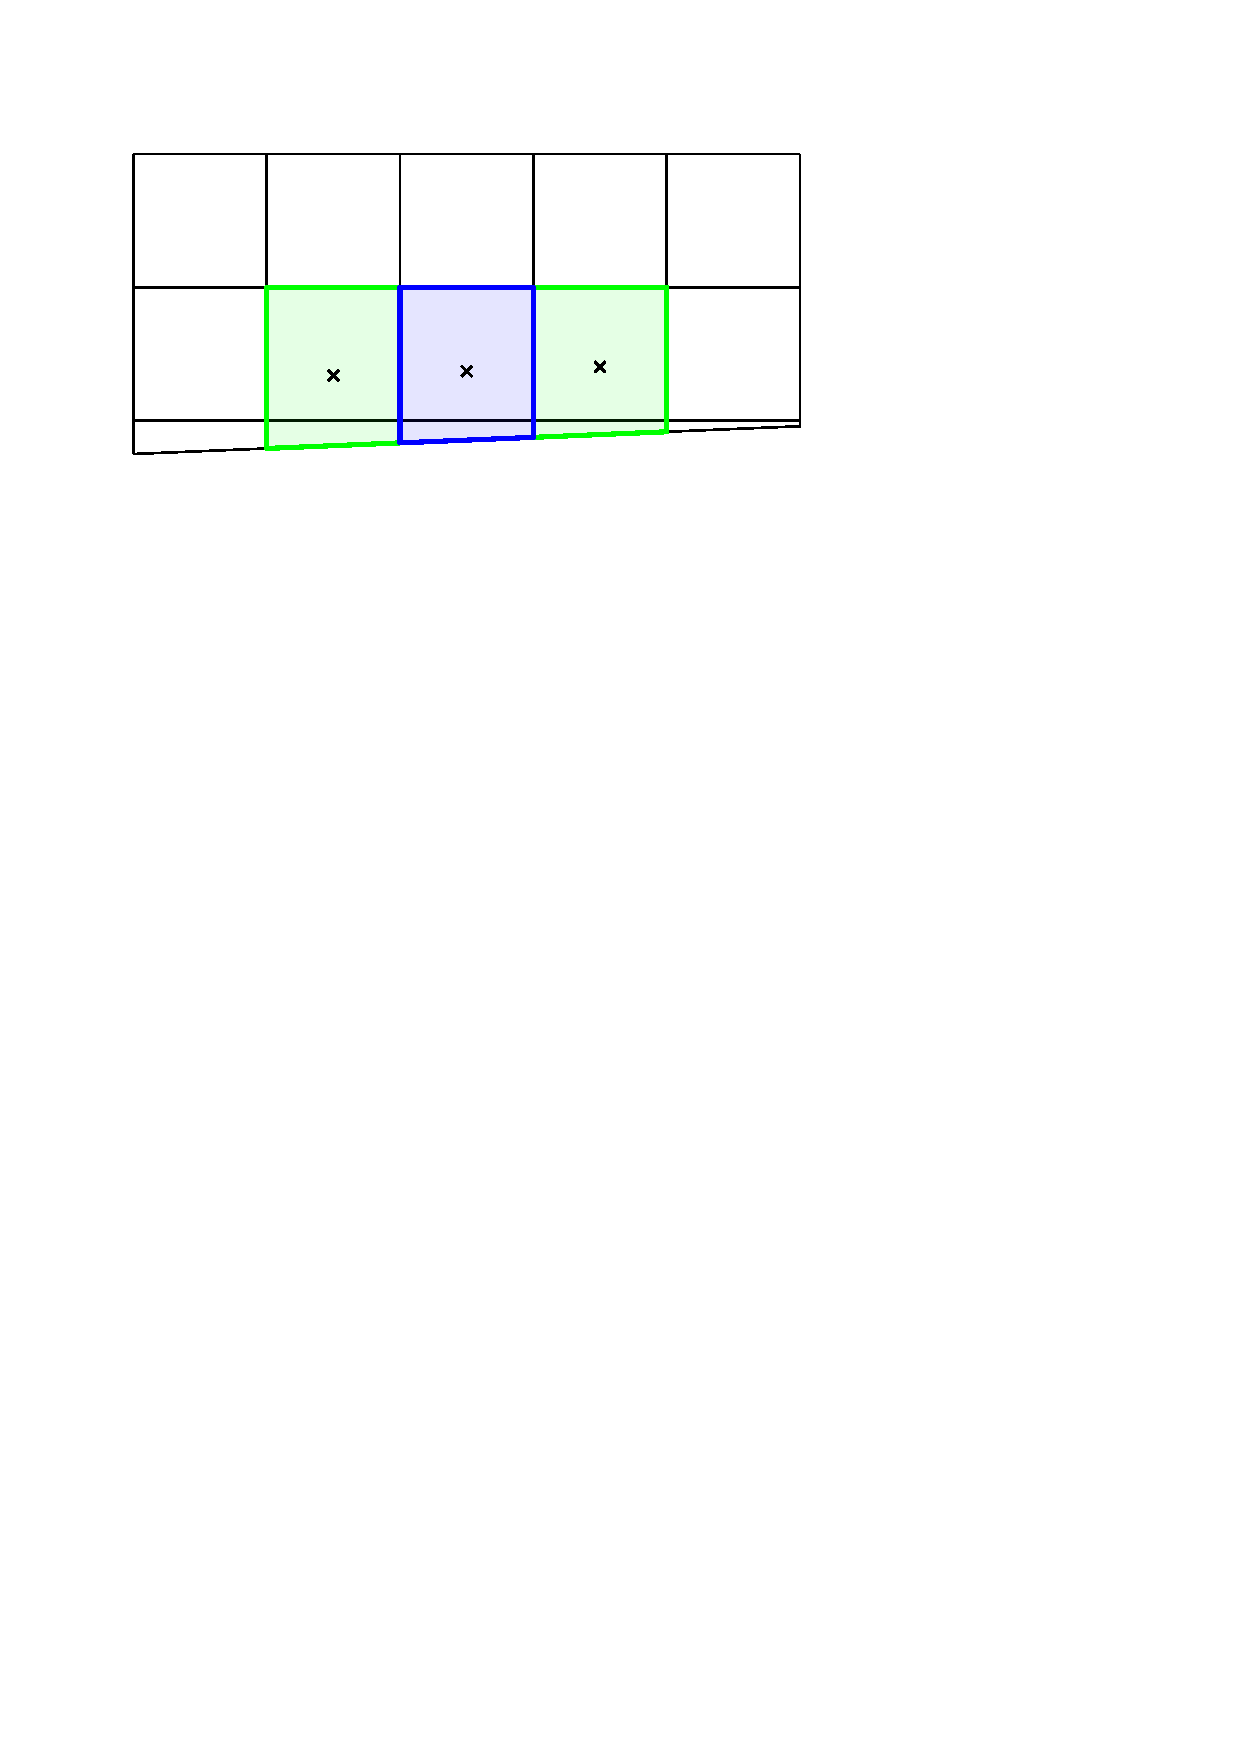
\includegraphics[width=0.45\linewidth]{figs/tooclose2.pdf}} \hfill
    \subfloat[]{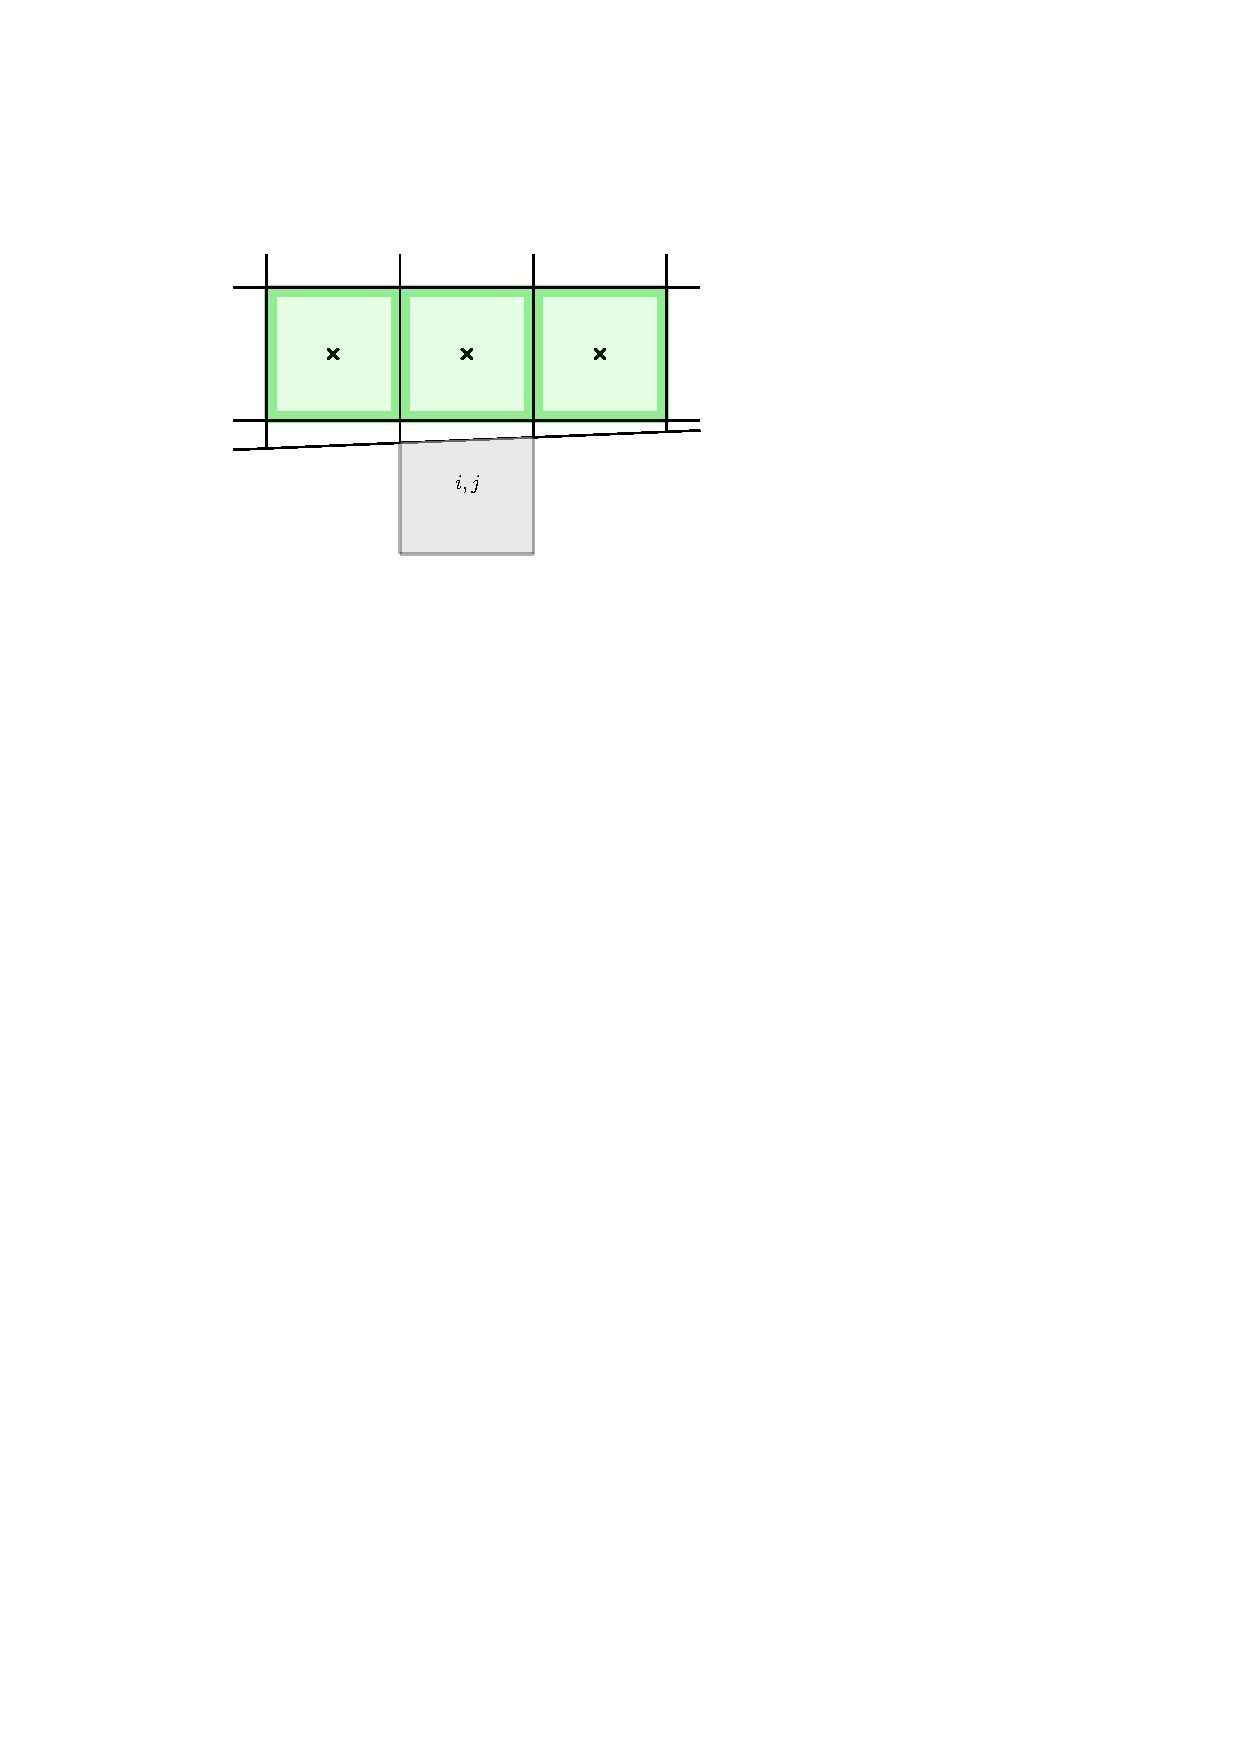
\includegraphics[width=0.45\linewidth]{figs/tooclose1.pdf}} 
    \caption{\sf The blue cell's $3\times3$ reconstruction tile highlighted in green.  The weighted centroids are indicated with a cross ($\times$).}
    \label{fig:tooclose}
\end{figure}

\item
{\bf Replace the provisionally computed cut cell values and their adjacent
full cell neighbors with  the contributions from the merged tiles.} 

\vspace*{.1in}
The final solution at time $t^{n+1}$ on cut cell $i,j$ is obtained by compiling a the indices of all merging neighborhoods that overlap cell $i,j$ in the set $W_{i,j}$.  Then, the solution on merging neighborhood $k,l$ in $W_{i,j}$ is evaluated at $i,j$'s physical centroid, $x_{i,j}$, given by $\hat{q}_{k,l}(x_{i,j})$.  The final solution value on cell $i,j$ is given by the average of these values, i.e.,
\begin{equation} \label{eq:final_update_linear}
U^{n+1}_{i,j} := \frac{1}{N_{i,j}}\sum_{(k,l) \in W_{i,j}}\hat{q}_{k,l}(x_{i,j}).
\end{equation}
To use the example of figure \ref{fig:2nborTile}, the cut cell value
\begin{equation}
   U_{i,j}^{n+1} := \widehat{Q}_{i,j} 
   + (x_m - x_{i,j}) \, \frac{\partial \widehat{Q}_{i,j}}{\partial x} 
   + (y_m - y_{i,j}) \, \frac{\partial \widehat{Q}_{i,j}}{\partial y}
\end{equation}
since cell ${i,j}$ only belongs to one neighborhood. The adjacent full cell
on the other hand belongs to two neighborhoods -- the one it shares with
the cut cell $i,j$ , and its own merging neighborhood.
So its solution at time $t_{n+1}$  becomes
\begin{equation}
\label{eqn:numhood2ex}
\begin{split}
   U_{i,j+1}^{n+1} \,=\, & \frac{1}{2}\widehat{q}_{i,j}(x_{i,j})+ \frac{1}{2} \widehat{q}_{i,j+1}(x_{i,j}), \\
   = &\frac{1}{2} \left
   (\widehat{Q}_{i,j} 
   + (x_m - x_{i,j+1}) \, \frac{\partial \widehat{Q}_{i,j}}{\partial x} 
   + (y_m - y_{i,j+1}) \, \frac{\partial \widehat{Q}_{i,j}}{\partial y} \right ) + \frac{1}{2} \widehat{Q}_{i,j+1} .
\end{split}
\end{equation}
The last term  in eq. \eqref{eqn:numhood2ex} has no gradient terms because the
centroids of the original cell and merged cell are identical.
The fraction $\frac{1}{2}$ is because cell $(i,j+1)$ is part of  two
neighborhoods, so each contributes half of the solution.
\end{enumerate}

Different choices of neighborhoods, the minimum volume for the merging
neighborhood, gradient neighborhoods, and limiting will give
somewhat different computational results. Some of these will be examined
theoretically using model problems in one space dimension in section
\ref{sec:theory}. These choices can affect the stability limit of the
overall method.
We will also show computational results using different neighborhood
choices in section \ref{sec:compResults} in two space dimensions.

The conservation properties of the algorithm will be discussed after the
higher order SRD algorithm is presented in the next
section (PR PUT IT HERE). It will also be prseented more generally.   
OTHER THINGS HERE? DEMONSTRATE LINEARLY EXACT SECOND ORDER CONVERGENCE
HERE INSTEAD OF COMPRESULTS SECTION?

% SOMEHWERE PUT IMPLEMENTATION SUBSECTION OR AT LEAST A PARAGRAPH
% TO NOTE THAT THE CELL DOESNT KNOW WHO GIVES TO
% IT, SO THIS LOOP IS OVER GIVERS  NOT RECEIVERS.
The final update formula \eqref{eq:final_update_linear} can easily be implemented with a nested for loop in algorithm \ref{alg:finalupdate}.  
The outer loop iterates over the merging neighborhoods $i,j$ and the inner loop iterates over each cell $k,l$ in merging neighborhood $i,j$.  Each merging neighborhood $i,j$ gives a contribution $ \hat{q}_{i,j}(x_{k,l})/N_{k,l} $ to the cells $k,l$ that belong to it.
\begin{algorithm}[H]
\SetAlgoLined
$U^{n+1}(:,:) := 0$\\
 \ForAll{$i,j$}{
     \ForAll{$(k,l) \in M_{i,j}$}{
        $U^{n+1}(k,l) := U^{n+1}(k,l) + \hat{q}_{i,j}(x_{k,l})/N_{k,l} $
     }
 }
 \caption{\sf Final solution update} \label{alg:finalupdate}
\end{algorithm}

\begin{figure}
	\subfloat[]{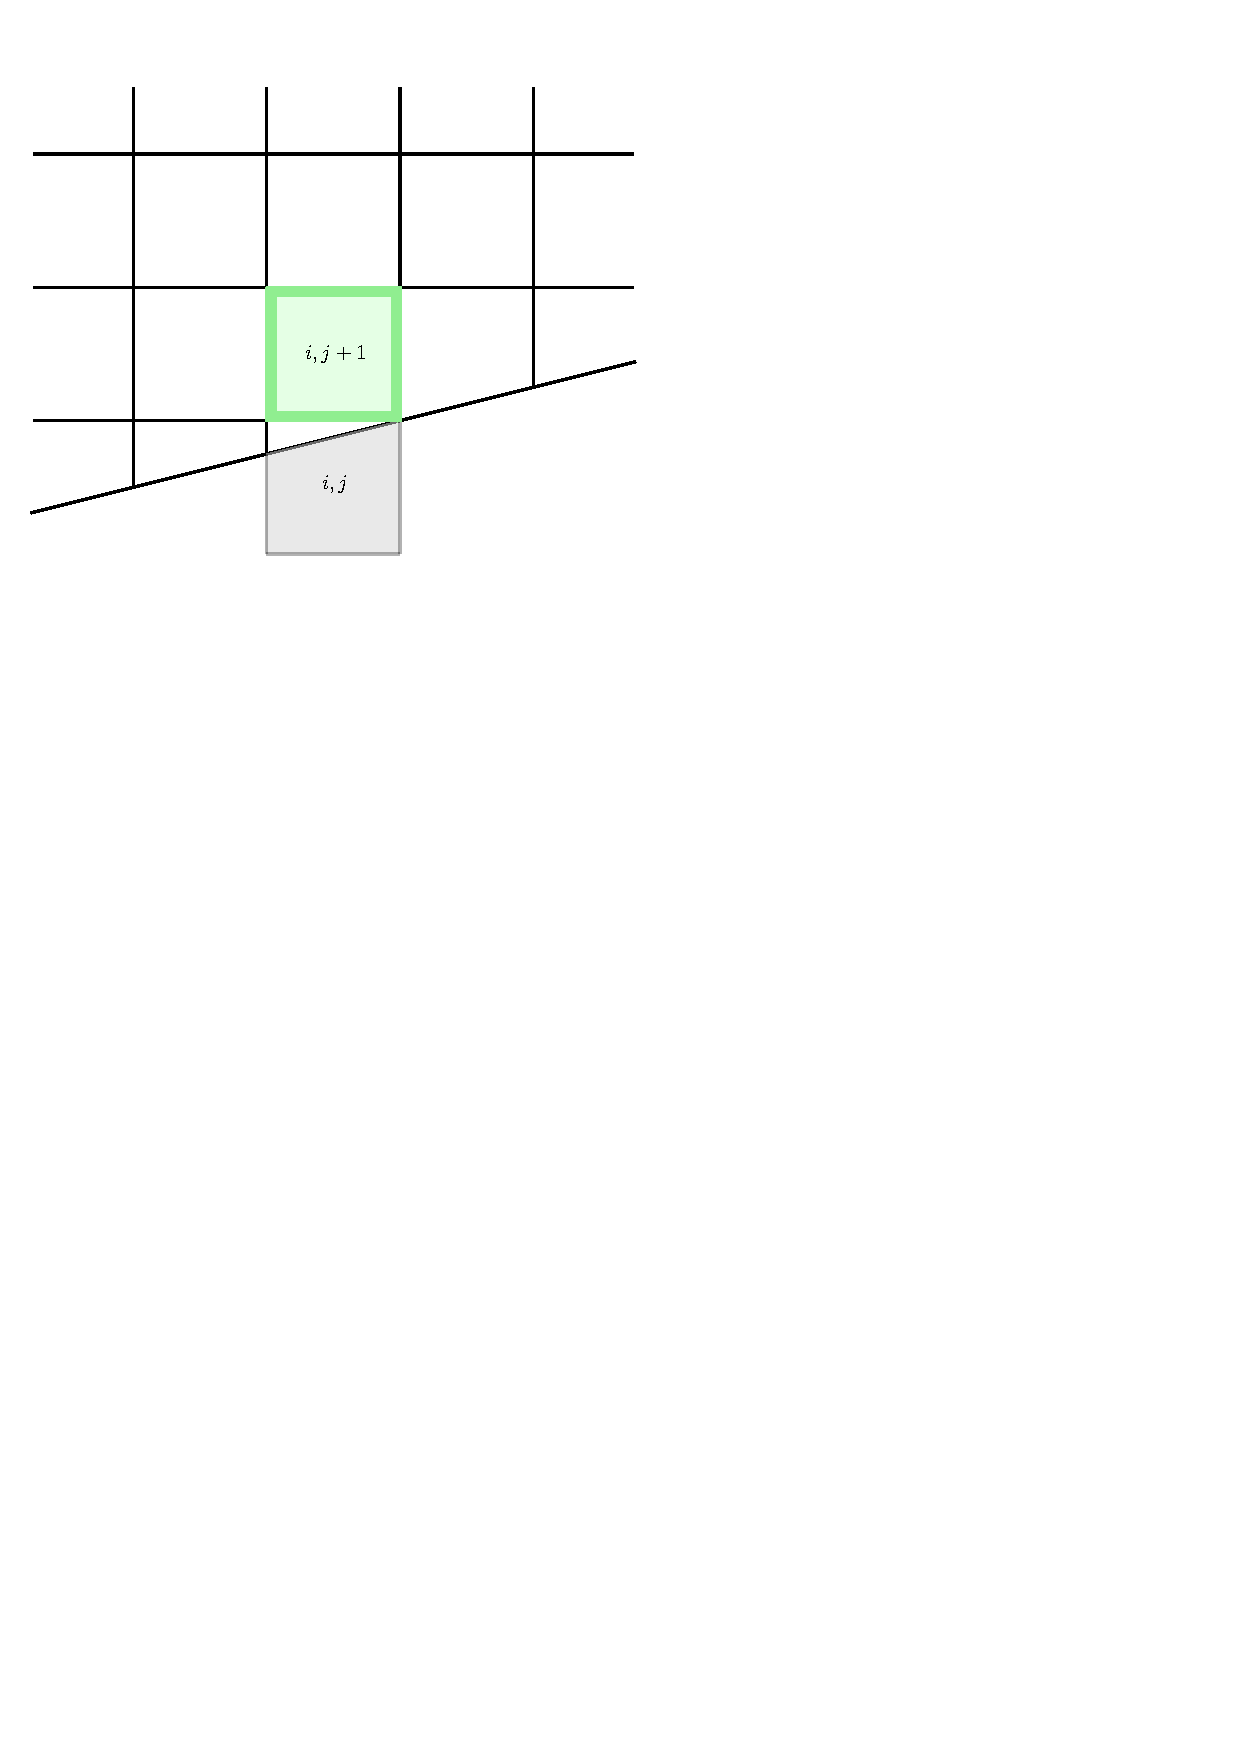
\includegraphics[width=0.45\textwidth]{figs/modelexample2D_1.pdf} \label{fig:2nborTile1}}
	\hfill
	\subfloat[]{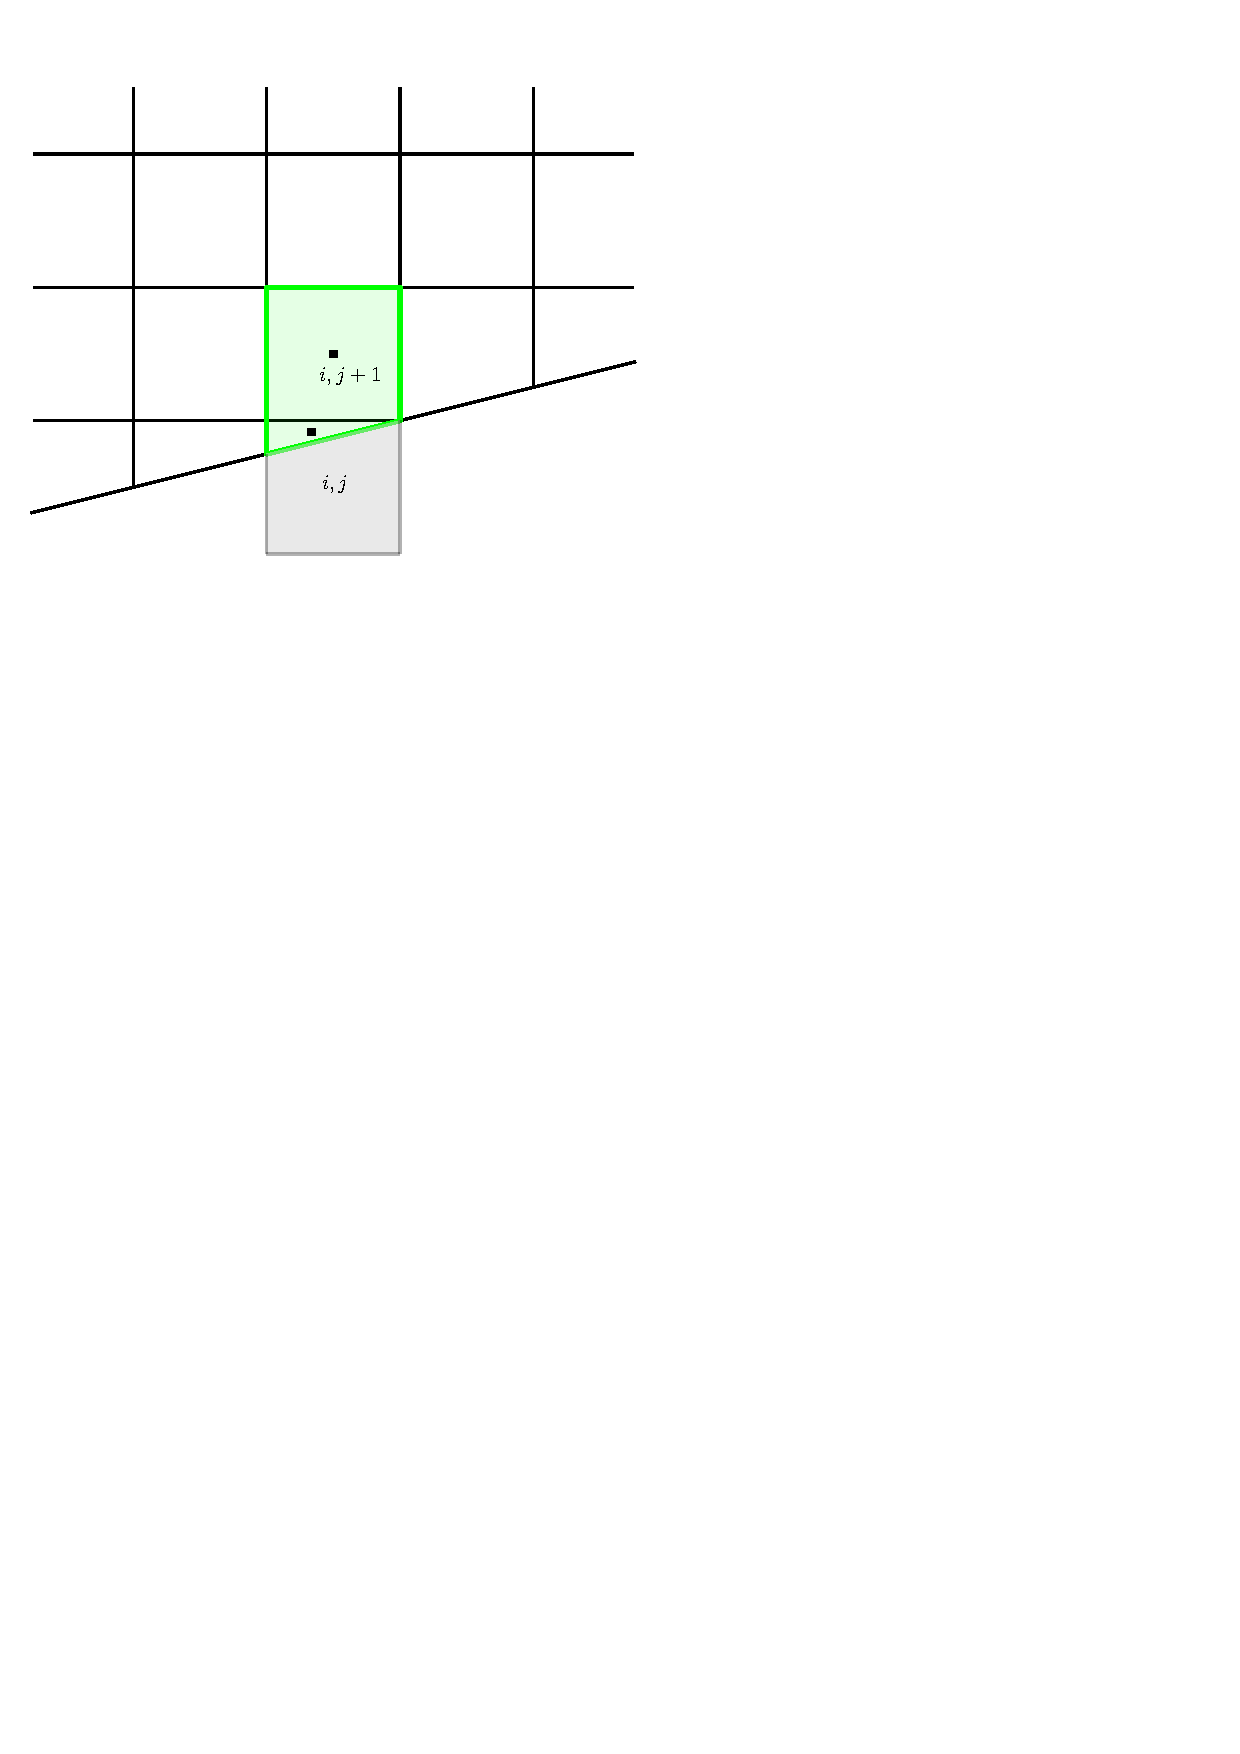
\includegraphics[width=.45\textwidth]{figs/modelexample2D_2.pdf} \label{fig:2nborTile2}}
	\caption{\sf Two-dimensional example of overlapping neighborhoods.  The unweighted centroids of cells $i,j$ and $i,j+1$ are indicated with solid squares ($\blacksquare$).} \label{fig:2nborTile}
\end{figure}


\subsection{Limiting on merging neighborhoods}
In this section we design a linearity preserving limiter for slopes on merging neighborhoods.  Designing a limiter that does not destroy the linearly preserving property is not so straightforward.  
%We demonstrate this
%In particular, we apply the LP limiter [] on slopes


\section{Computational Results}\label{sec:compResults}
In this section we show several computational experiments using state
redistribution to solve the Euler
equations. We will also use these
examples to examine 
properties of different gradient choices and base schemes. 
%We solve the conservation law \eqref{eq:conslaw2D} with different fluxes $\mathbf{F}$, to include both smooth and discontinuous
%solutions.

%\subsection{Linear fluxes}
%\subsubsection{Linear convergence study}
%We solve \eqref{eq:conslaw2D} with the flux $\mathbf{F}(u) = [-2\pi y u, 2\pi x u]$ and initial condition
%$$
%u_0(x,y) = w(\theta - \pi/2)
%$$
%where
%$$
%w(\theta) = \frac{1}{2}\left( \text{erf}\left( \frac{\pi/6 - \theta}{\sqrt{4/100}} \right) + \text{erf}\left( \frac{\pi/6 + \theta}{\sqrt{4/100}} \right)\right)
%$$
%until the final time $T = 1$ on the domain enclosed by two concentric disks of 
%radii $R_1 = 0.751$ and $R_2 = 1.251$.  
%Figure \ref{fig:rotatinghillgrid} shows the computational domain 
%embedded in a $50 \times 50$ grid.  The exact solution is the initial condition 
%rotated about the point $(1.5,1.5)$, where $T=1$ corresponds to one solid 
%body rotation. This example IS FROM \cite{}, for comparison.  (AND ADD
%COMPARISON - ARE THEY OR WE MORE ACCURATE< BUT WE ARE EASIER).   
%The errors 
%measured in the $L_1$ and $L_\infty$ norms are provided in 
%Tables \ref{tab:ex1_L1} and \ref{tab:ex1_Linf}.  Figure
%\ref{fig:rotatinghillexactiso} shows isolines of solution at the initial 
%and final time.  The exact solution is applied as the boundary condition.
%CHEATING?
%This problem is solved using the finite volume TVD-RK2 scheme. 
%
%\begin{figure}
%\subfloat[$50\times50$ grid and annulus domain.]{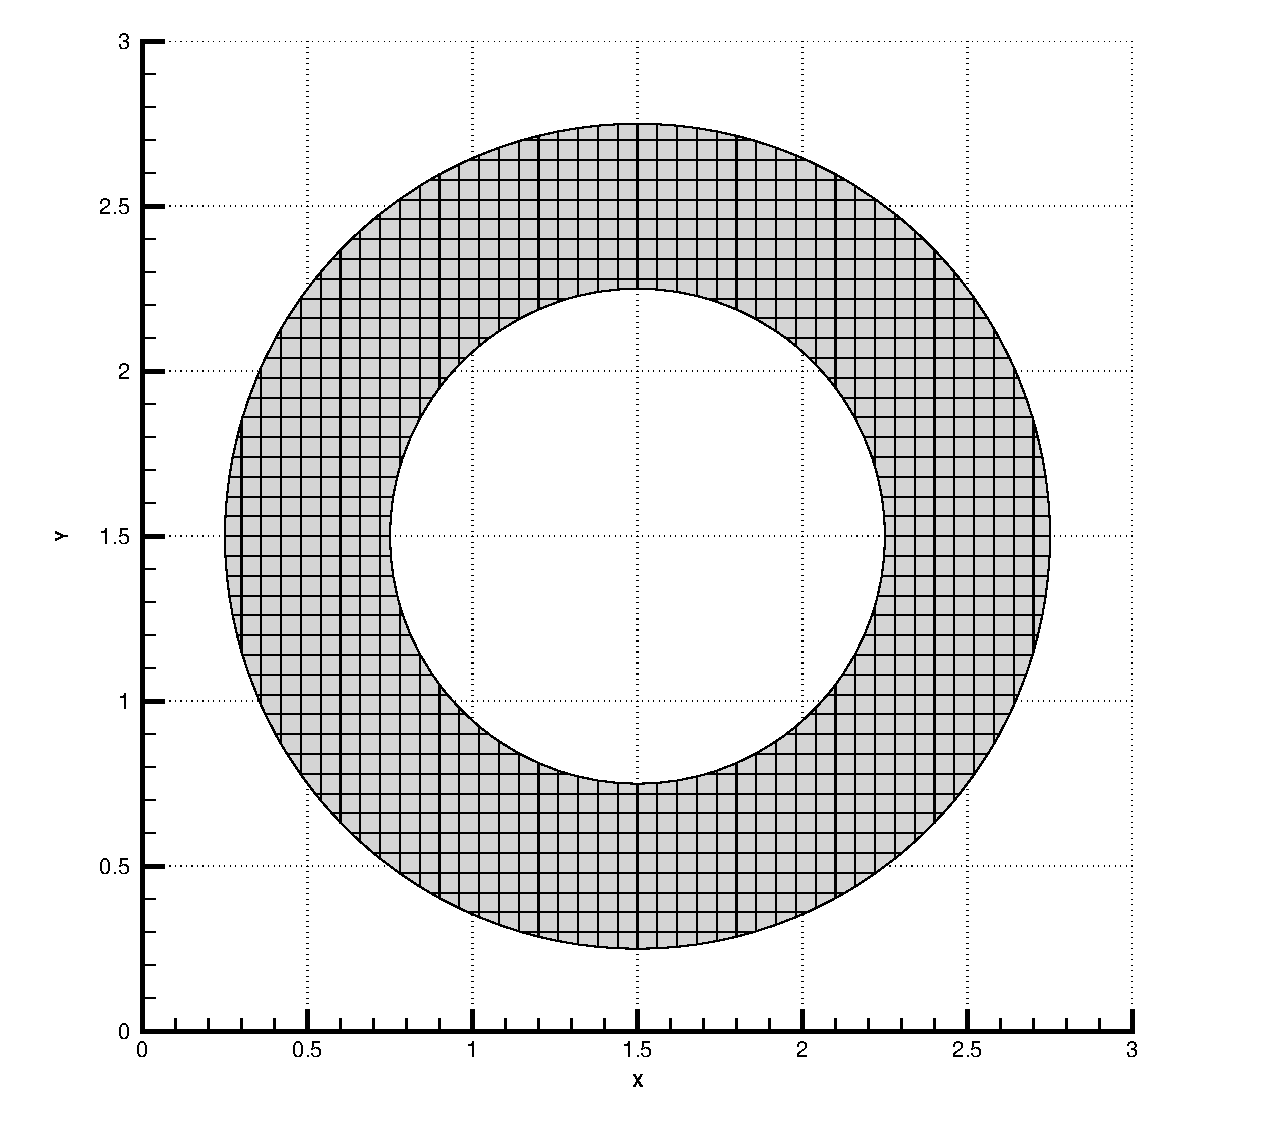
\includegraphics[width = 0.5\linewidth]{figs/rotatinghill_grid.eps} \label{fig:rotatinghillgrid}} 
%\quad
%\subfloat[Isolines of exact solution at the initial and final time. SHOW
%COMPUTED SOLUTION TOO]{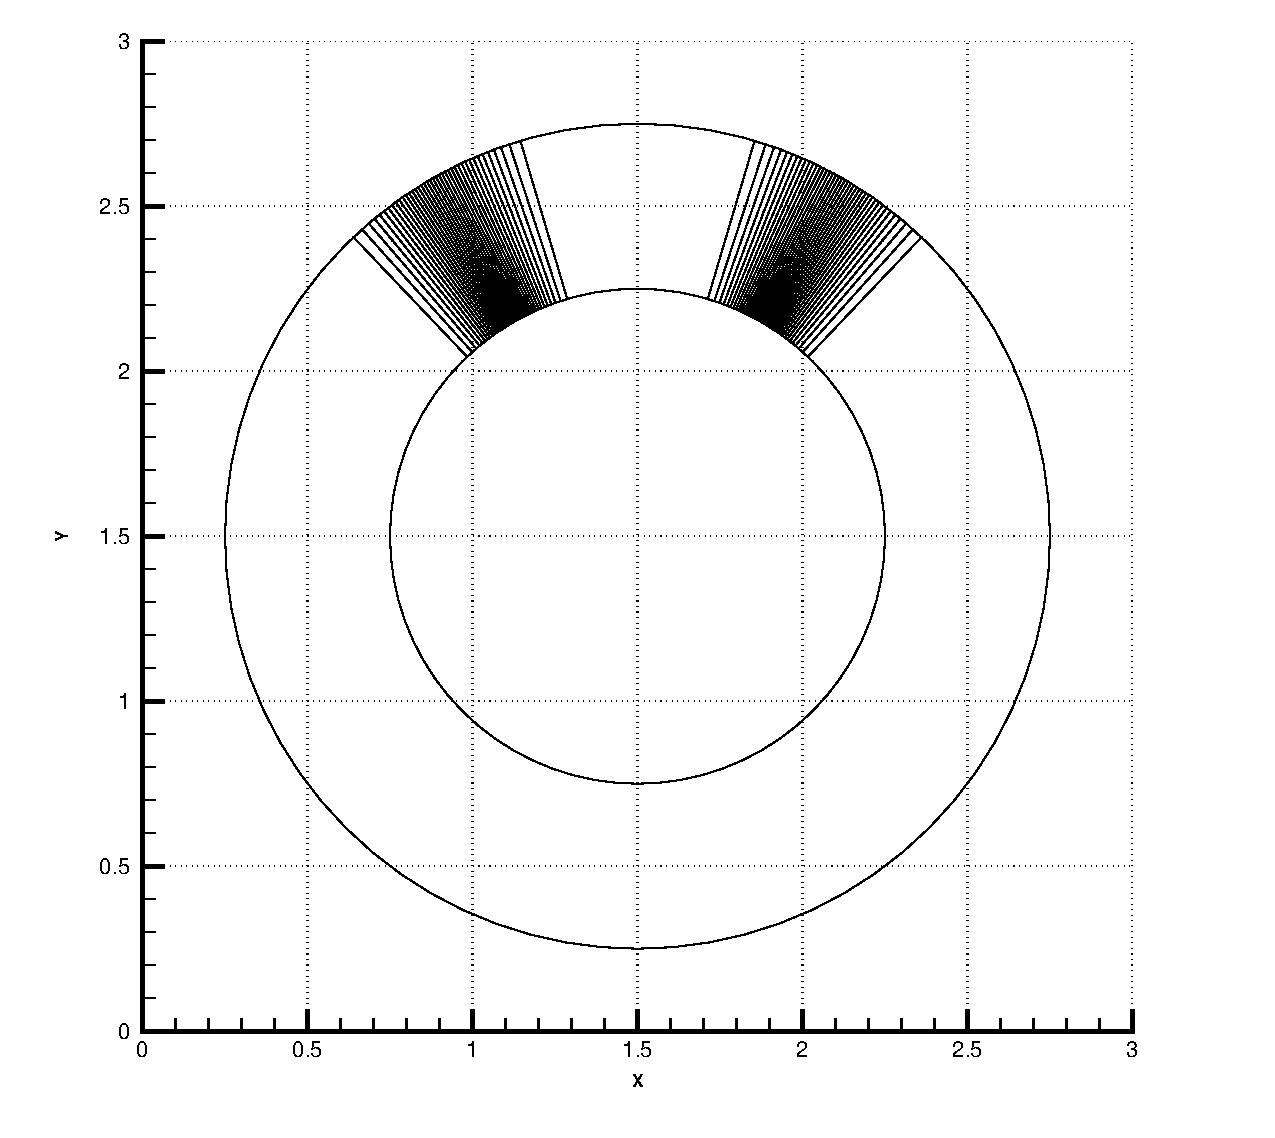
\includegraphics[width = 0.5\linewidth]{figs/rotatinghill_solution.eps}\label{fig:rotatinghillexactiso}}
%\end{figure}
%    % \caption{}\label{tab:ex1_L1}
%
%{\large
%\begin{table}
%\centering
%\subfloat[$L_1$ errors. \label{tab:ex1_L1}]{
%    \begin{tabular}{|c|c|c|c|c|}
%        \hline
%         $N_x \times N_y$ & $p = 0$ & $p=1$& $p=2$ & $p=3$ \\
%         \hline
%         50 & 2.3937e-1(-) &  5.6588e-2  (-)& 4.1690e-2  (-)&   2.0694e-2 (-)\\
%         \hline
%         100 &  1.5521e-1 (0.62) &  2.0125e-2  (1.49)& 7.8165e-3 (2.41)& 1.6813e-3 (3.62)\\
%         \hline
%         200 &  9.4138e-2 (0.72) & 5.5222e-3 (1.86)&  9.98411e-4 (2.96)& 8.8527e-5 (4.24)\\
%        %  \hline
%        %  400 &  () &  ()&  ()&  ()\\
%         \hline
%    \end{tabular}
%    }
%\quad
%\subfloat[$L_\infty$ errors. \label{tab:ex1_Linf}]{
%    \begin{tabular}{|c|c|c|c|c|}
%        \hline
%         $N_x \times N_y$ & $p = 0$ & $p=1$& $p=2$ & $p=3$ \\
%         \hline
%         50 & 3.0385e-1 (-) &  1.6856e-1 (-)& 1.1809e-1 (-)&  7.0682e-2 (-)\\
%         \hline
%         100 & 2.3332e-1 (0.38) & 8.5487e-2 (1.04)& 5.1249e-2 (1.20)& 1.6657e-2 (2.08)\\
%         \hline
%         200 &  1.7698e-1 (0.39) & 3.4940e-2 (1.29)& 1.4500e-2 (1.82)&  1.9507e-3 (3.09)\\
%        %  \hline
%        %  400 &   () &  ()&  ()&  ()\\
%         \hline
%    \end{tabular}
%    }
%
%\caption{Errors for the linear convergence study. ADD METHOD DETAILS TO
%DESCRIPTION - USED WHICH GRADIENT RECON. ADD 400 POINTS}
%\end{table}
%}
%
%\subsubsection{Overlapping neighborhoods}
%The purpose of this example is to demonstrate that our algorithm can handle a substantial number of overlapping neighborhoods.  
%Using the streamfunction
%$$
%\phi = R - 0.25\sin(10\theta),
%$$
%with $R = \sqrt{(x-1.5)^2+(y-1.5)^2}$ and $\theta = \arctan((y-1.5)/(x-1.5))$, we define a linear flux based on the resulting divergence free velocity field, i.e.,  $\mathbf{F}(u) = [\phi_y u, -\phi_xu]$.  The characteristics of \eqref{eq:conslaw} lie on the isolines of the streamfunction.
%
%A steady state solution to \eqref{eq:conslaw} with the above flux is given by the streamline function.  Therefore, we start with the initial condition given by the streamline function $\phi$, and compute the solution until the final time $T = 10$ on a $100 \times 100$ grid.  Additionally, we set the flux normal the domain boundary $\mathbf{F}\cdot \mathbf{n} = 0$.  This is to ensure that information does not leave the domain and should solution growth occur, this will more easily be noticed.
%This problem is solved using the finite volume TVD-RK2 scheme. 
%
%
%\begin{table}[h]
%    \centering
%    \subfloat[$L_1$ errors.]{
%    \begin{tabular}{|c|c|c|c|}
%    \hline
%        $p = 0$ & $p =1$ & $p = 2$ & $p =3$  \\
%        \hline
%        3.8585e-1 & 3.6118e-2 & 8.29907e-3 & 4.3116e-3\\
%        \hline
%    \end{tabular} \label{tab:errorsteadystatel1}
%    }
%    \quad
%\subfloat[$L_\infty$ errors.]{
%    \begin{tabular}{|c|c|c|c|}
%    \hline
%        $p = 0$ & $p =1$ & $p = 2$ & $p =3$  \\
%        \hline
%        2.9470e-1 & 9.5323e-2 & 2.4851e-2 &  5.4720e-3 \\
%        \hline
%    \end{tabular}
%    \label{tab:errorsteadystatelinfty}
%    }
%    
%\caption{Errors for overlapping neighborhoods study.} \label{tab:overlappingerrors}
%\end{table}
%
%\begin{figure}[h]
%%\subfloat[Isolines of exact solution at the initial and final time.]{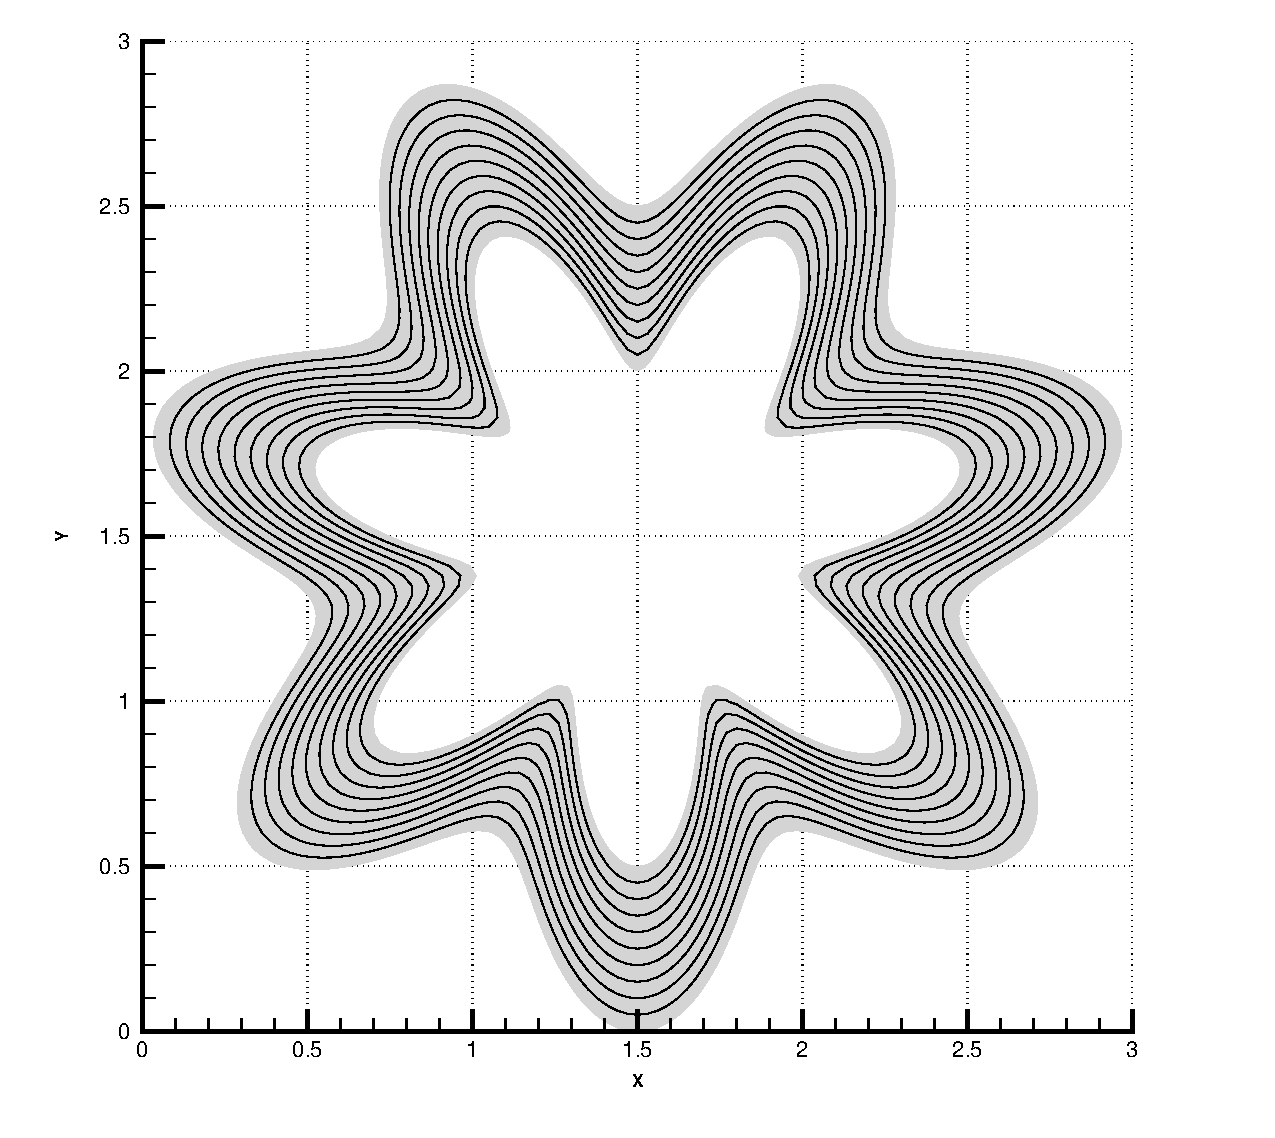
\includegraphics[width = 0.5\linewidth]{figs/waveyiso.eps} \label{fig:waveyisolines}} 
%%\subfloat[Isolines of exact solution at the initial and final time.]{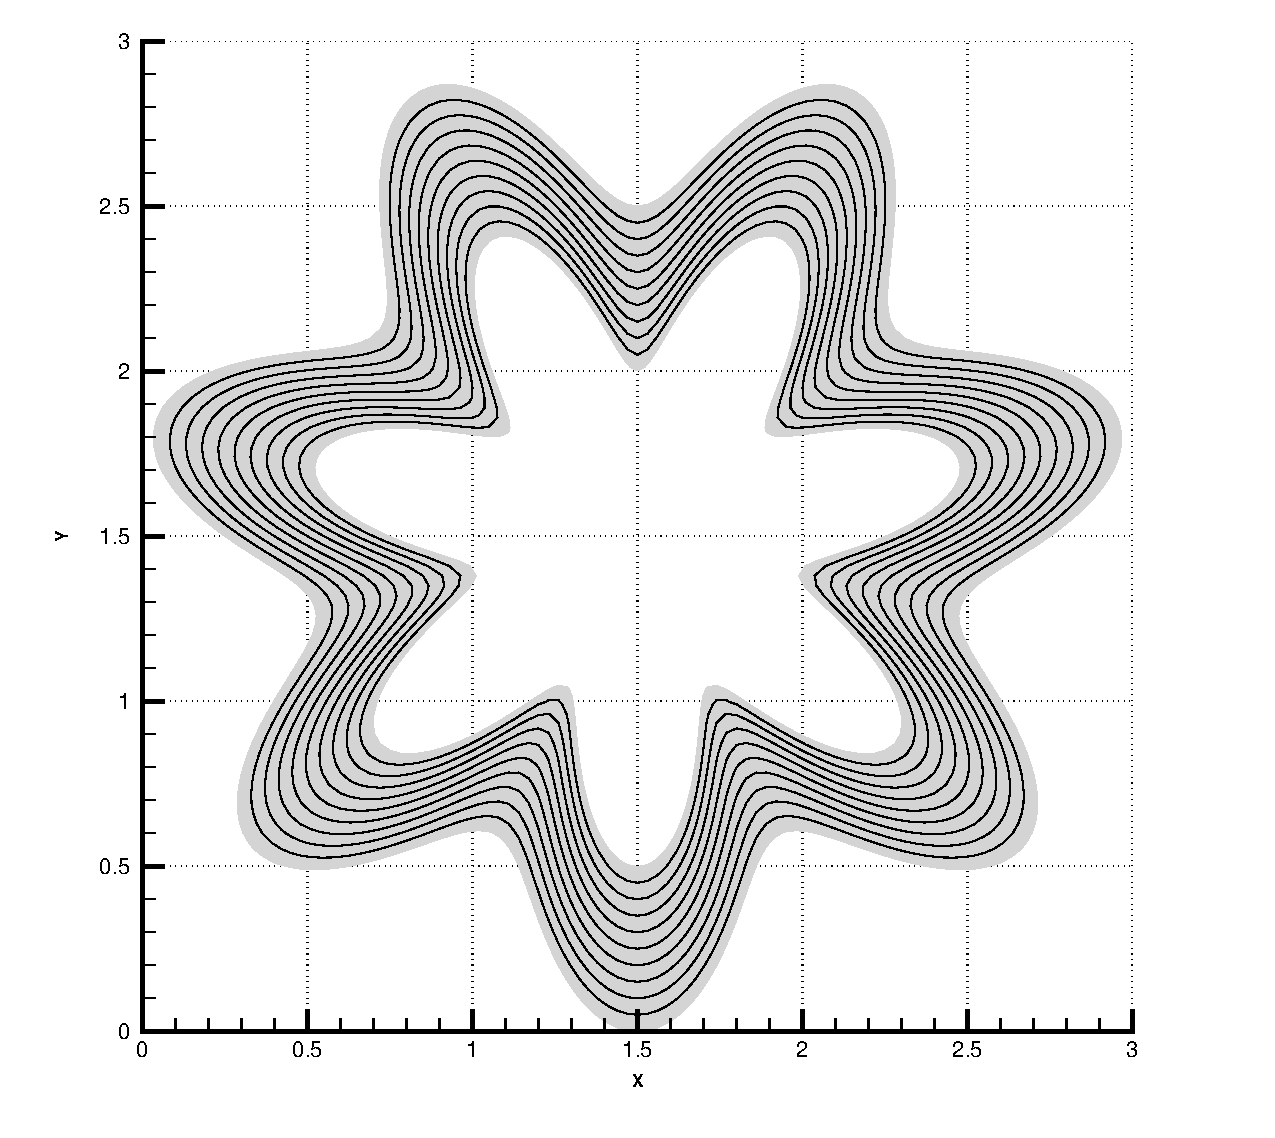
\includegraphics[width = 0.5\linewidth]{figs/waveyiso.eps} \label{fig:waveyisolines}} 
%%\quad
%\subfloat[Number of overlapping merging neighborhoods: one (blue), two (green), three (red).]{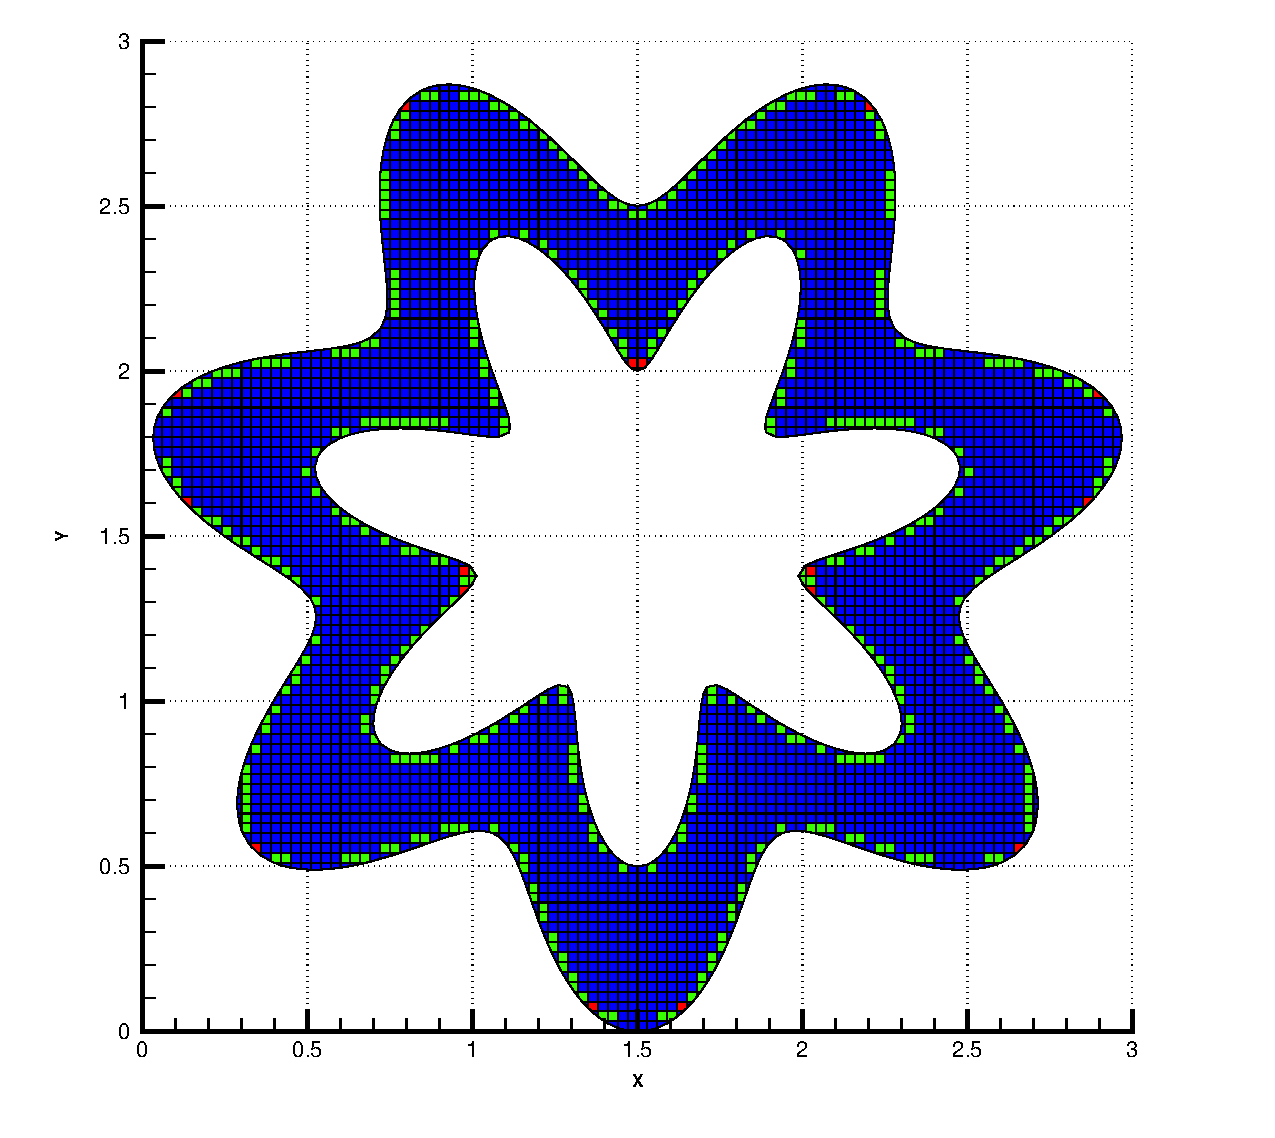
\includegraphics[width = 0.5\linewidth]{figs/waveynumhoods.eps}\label{fig:waveynumhoods}}
%% 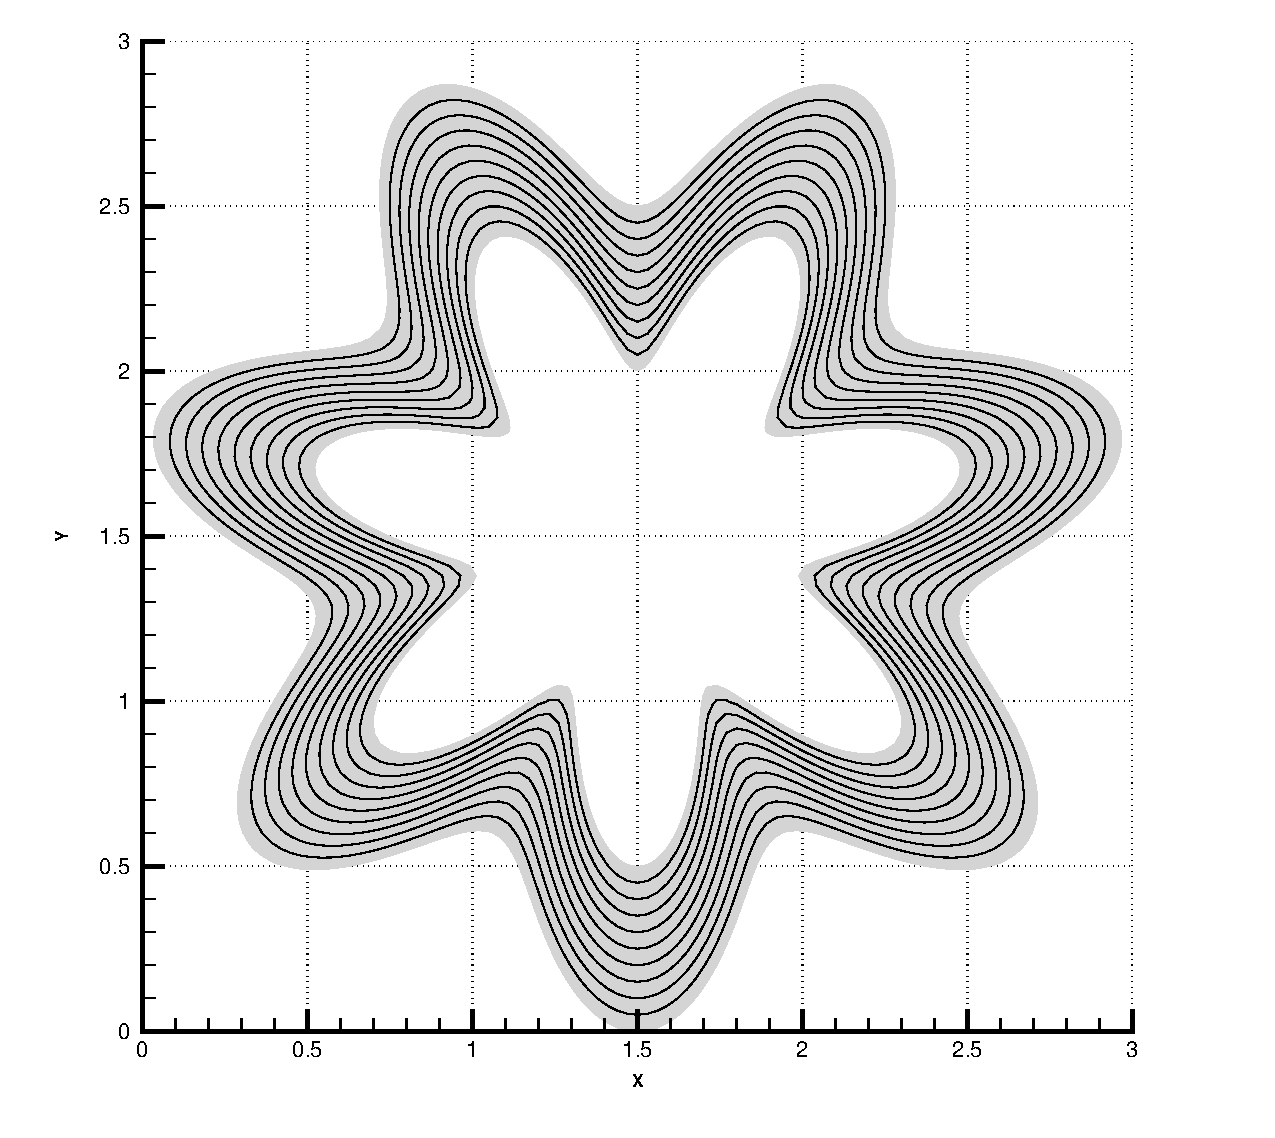
\includegraphics[width = 0.5\linewidth]{figs/waveyiso.eps} 
%\subfloat[Isolines of exact solution at the initial and final time.]{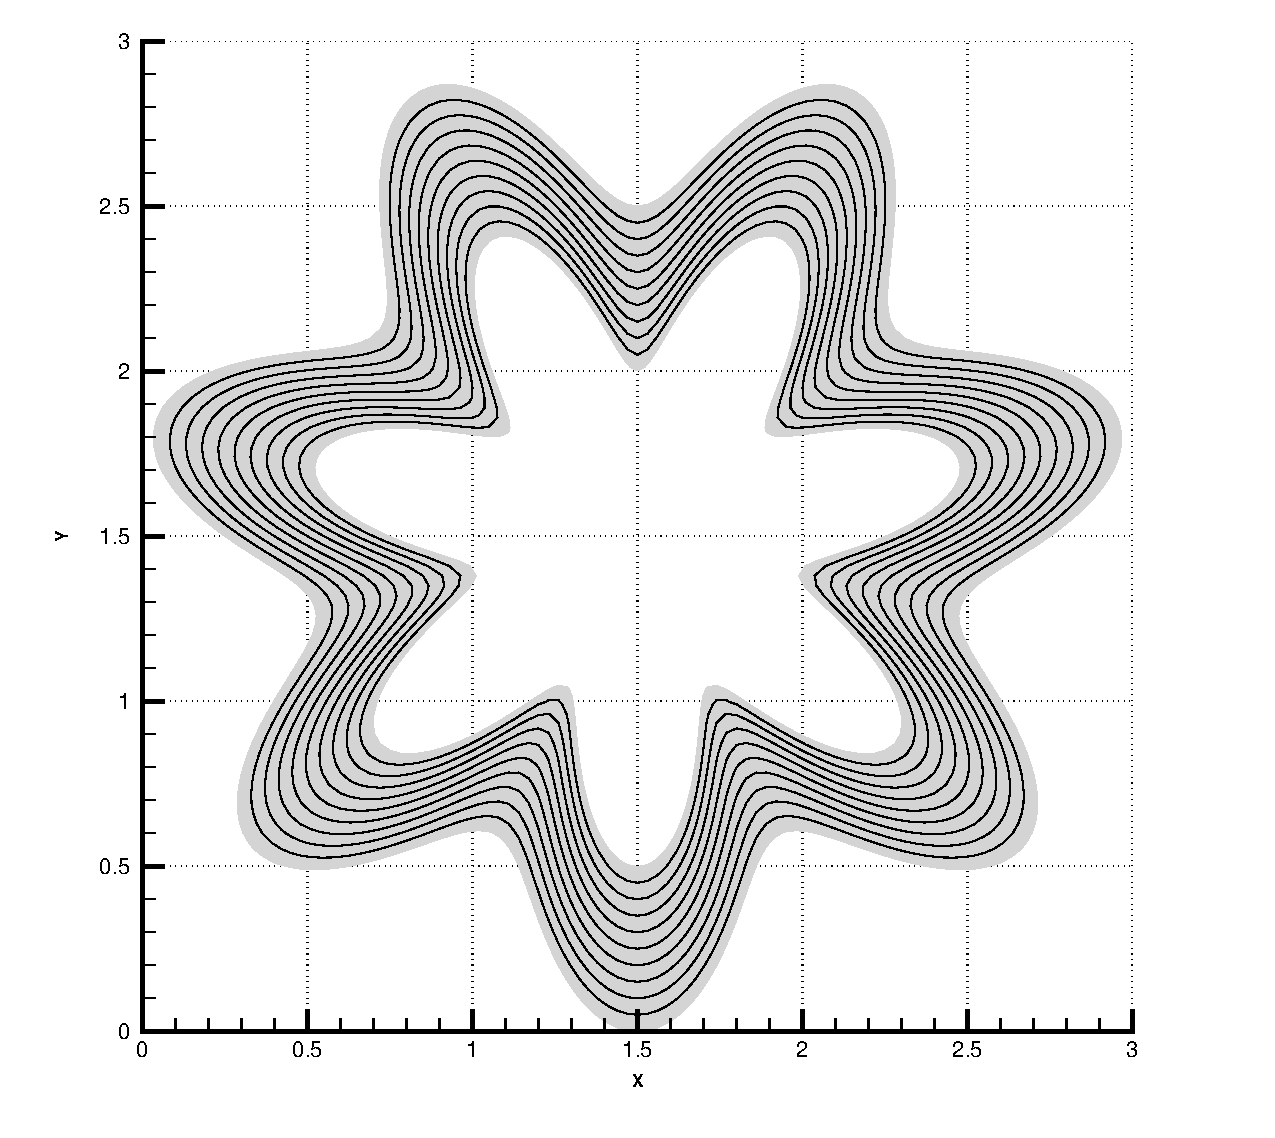
\includegraphics[width = 0.5\linewidth]{figs/waveyiso.eps} \label{fig:waveyisolines}} 
%\caption{Isolines of exact solution at the initial and final time for the
%wavy domain with overlapping neighborhoods. CANT SEE COLORS. WHAT DOES
%THIS EX ADD FROM PREVIOUS ONE} 
%% \label{fig:overlappingneighborhoods}
%% \label{fig:waveyisolines}} 
%\end{figure}
%
%In Figure \ref{fig:waveyisolines}, we show the isolines of the exact solution at the initial and final times.  Additionally, Figure \ref{fig:waveynumhoods} shows the number of overlapping neighborhoods on each cell.  In this example, we have at most three overlapping neighborhoods.  They are concentrated where the boundary has high curvature.   We do not observe growth in the numerical solution as indicated by $L_1$, $L_\infty$ errors of the solution at the final time listed in Table \ref{tab:overlappingerrors}.  Although this experiment does not prove stability of our numerical scheme, not observing unbounded growth in the numerical solution is a necessary condition.


\subsection{Supersonic vortex study}\label{sec:ssv}
We compute the solution to a supersonic flow 
around a quarter circle.  This problem has often been used in accuracy 
studies \cite{aftosmis:acc} since it has an exact solution to the Euler
equations that is smooth, given by 
\begin{equation}
\rho = \rho_i \left \{ 1 + \frac{\gamma-1}{2} \, M_i^2 \left [ 1 - (\frac{r_i}{r})^2
\right ] \right \} ^
{\frac{1}{\gamma-1}}
\end{equation}
and $ u = a_i \, M_i \, (\frac{r_i}{r})\,  \sin (\theta)$, 
$ v = a_i\,  M_i\,  (\frac{r_i}{r})\,  \cos(\theta)$, and
$ p = \rho^\gamma / \gamma$.
Here, the inner radius is $r_i = 1.0$,  the outer radius
is $r = 1.384$, $\rho_i=1$, and the Mach number on the inner circle
$M_i = 2.25$ in our experiments. 
In this
normalization we use $a_i = 1$, $p_i = 1/\gamma$. 
The second order MOL scheme is used, and we march
to steady state, until the maximum density update is below $10^{-10}$.  
The solution is smooth, so no limiters are needed.
The exact solution is used to set the ghost cells at the inflow and
outflow boundaries. The domain size is 1.43 by 1.4301 (slightly different
to prevent mesh  degeneracies).  

In Table \ref{tab:ssv} we compare the accuracy of three different formulations
for the cut cell gradients. 
For first order accurate gradients, we use a linear least squares reconstruction for
both the irregular cell gradient (cut cells and their one-away neighbors) 
described in Section \ref{sec:limit}, and the SRD gradients, which 
update the cut cell solution after stabilization. Second order accurate 
gradients fit a quadratic for both
the cut cells and tiles as described in Section \ref{sec:limit}, 
but only the first derivative terms are used. 
As an intermediate experiment, we  fit a quadratic using least squares but treating the
cell averages as pointwise values at the cell centers. Here again
the second derivative terms are ignored.  Note that this is not
second order accurate, since the centroid value differs by $O(h^2)$
from the pointwise value at the centroid. Nevertheless, this is frequently
done since it is easier to implement, in particular for the SRD neighborhoods
with irregular shapes. 



{
\small
\begin{table}[h]
\centering
	\hspace*{-.3in}
	\subfloat[$L_1$ volume errors. \label{tab:ex1_L1vol}]{
		\begin{tabular}{|l|c|l|l|l|}
			\hline
			$h$ & $N_x, N_y$ & 1st order grad. & ptwise grad. & 2nd order grad.   \\
			\hline
			.5297 & 27 & 6.75e-3 & 2.76e-3 & 2.45e-3 \\
			\hline
			.2648 & 54  & 1.78e-4 (3.8)  & 6.38e-4 (4.3) & 4.71e-4 (5.2) \\
			\hline
			.1324 &108 & 3.63e-4 (4.9)  & 1.53e-4 (4.2) & 1.21e-4 (3.9) \\
			\hline
			.662e-2 & 216 & 6.52e-5 (5.6)  & 3.65e-5  (4.2) & 2.98e-5 (4.1) \\
			\hline
			.331e-2 & 432 & 1.40e-5 (4.7)  & 8.85e-6  (4.1) & 7.86e-6 (3.8) \\
			\hline
			.166e-2 & 864 & 2.68e-6 (5.2)  & 2.15e-6  (4.1) & 2.04e-6 (3.9) \\
			\hline \hline
		\end{tabular}
	}
	\quad
	\vspace*{.2in}
	
	\hspace*{-.3in}
	\subfloat[$L_1$ boundary errors. \label{tab:ex1_L1bndry}]{
		\begin{tabular}{|l|c|l|l|l|l|}
			\hline
	    $h$ &  $N_x, N_y$   & 1st order grad.  & ptwise grad. &  2nd order grad.    \\
	\hline
     .5297 & 	27  &   6.84e-02 &  3.31e-02  & 2.37e-2\\
	\hline
     .2648 &	54  &   2.83e-02 (2.4) &  1.21e-02 (2.7)  & 8.183-3  (2.9) \\
	\hline
      .1324 &	108 &   1.03e-02  (2.8)&  4.69e-03 (2.6) & 3.453-3 (2.4) \\
	\hline
     .662e-2 &	216 &   3.65e-03  (2.8) &  1.82e-03 (2.6) & 1.38e-3 (2.5) \\
			\hline
    .331e-2 &	432 &   1.24e-03  (3.0)  &  7.18e-04 (2.6) & 6.15e-4 (2.2) \\
			\hline
    .166e-2 &	864 &   3.96e-04  (3.1)  &  2.85e-04 (2.6) & 2.58e-4 (2.4) \\
			\hline \hline
		\end{tabular}
	}
	
	\caption{\sf L1 norm of the error in the domain volume and along the boundary,
        for the supersonic vortex example. The error using first order accurate
        gradients, pointwise quadratic, and fully second order accurate gradients is shown. 
        Pointwise quadratic gradients have half of the error than first order gradients. 
        Truly second order accurate gradients are even better, especially on coarser grids. \label{tab:ssv}}
\end{table}
}

We measure the $L_1$ norm of the error in the volume,   $\sum_{i,j} \,
V_{ij} \lvert e_{ij } \rvert$ and at the boundary, $ \sum_{{i,j} \in \partial \Omega} \, A_{ij} \lvert e_{ij
} \rvert$.  Here
$e_{i,j}$ is the error at the cell centroid, and $A_{ij}$ is the length of the 
boundary segment in cut cell $(i,j)$.
These are given in Table \ref{tab:ex1_L1vol} and \ref{tab:ex1_L1bndry}. 
For easier comparison with other papers we also give the mesh size 
to a few digits. In  a cut cell mesh there are both solid and
flow cells, so the total number of cell is larger than the number of
flow cells, and not as easy to compare as the mesh spacing.
All interior cells use the evolution scheme and gradients, so
the difference in the errors are solely due to the cut cell gradients.

\begin{figure}[h]
	\begin{center}
		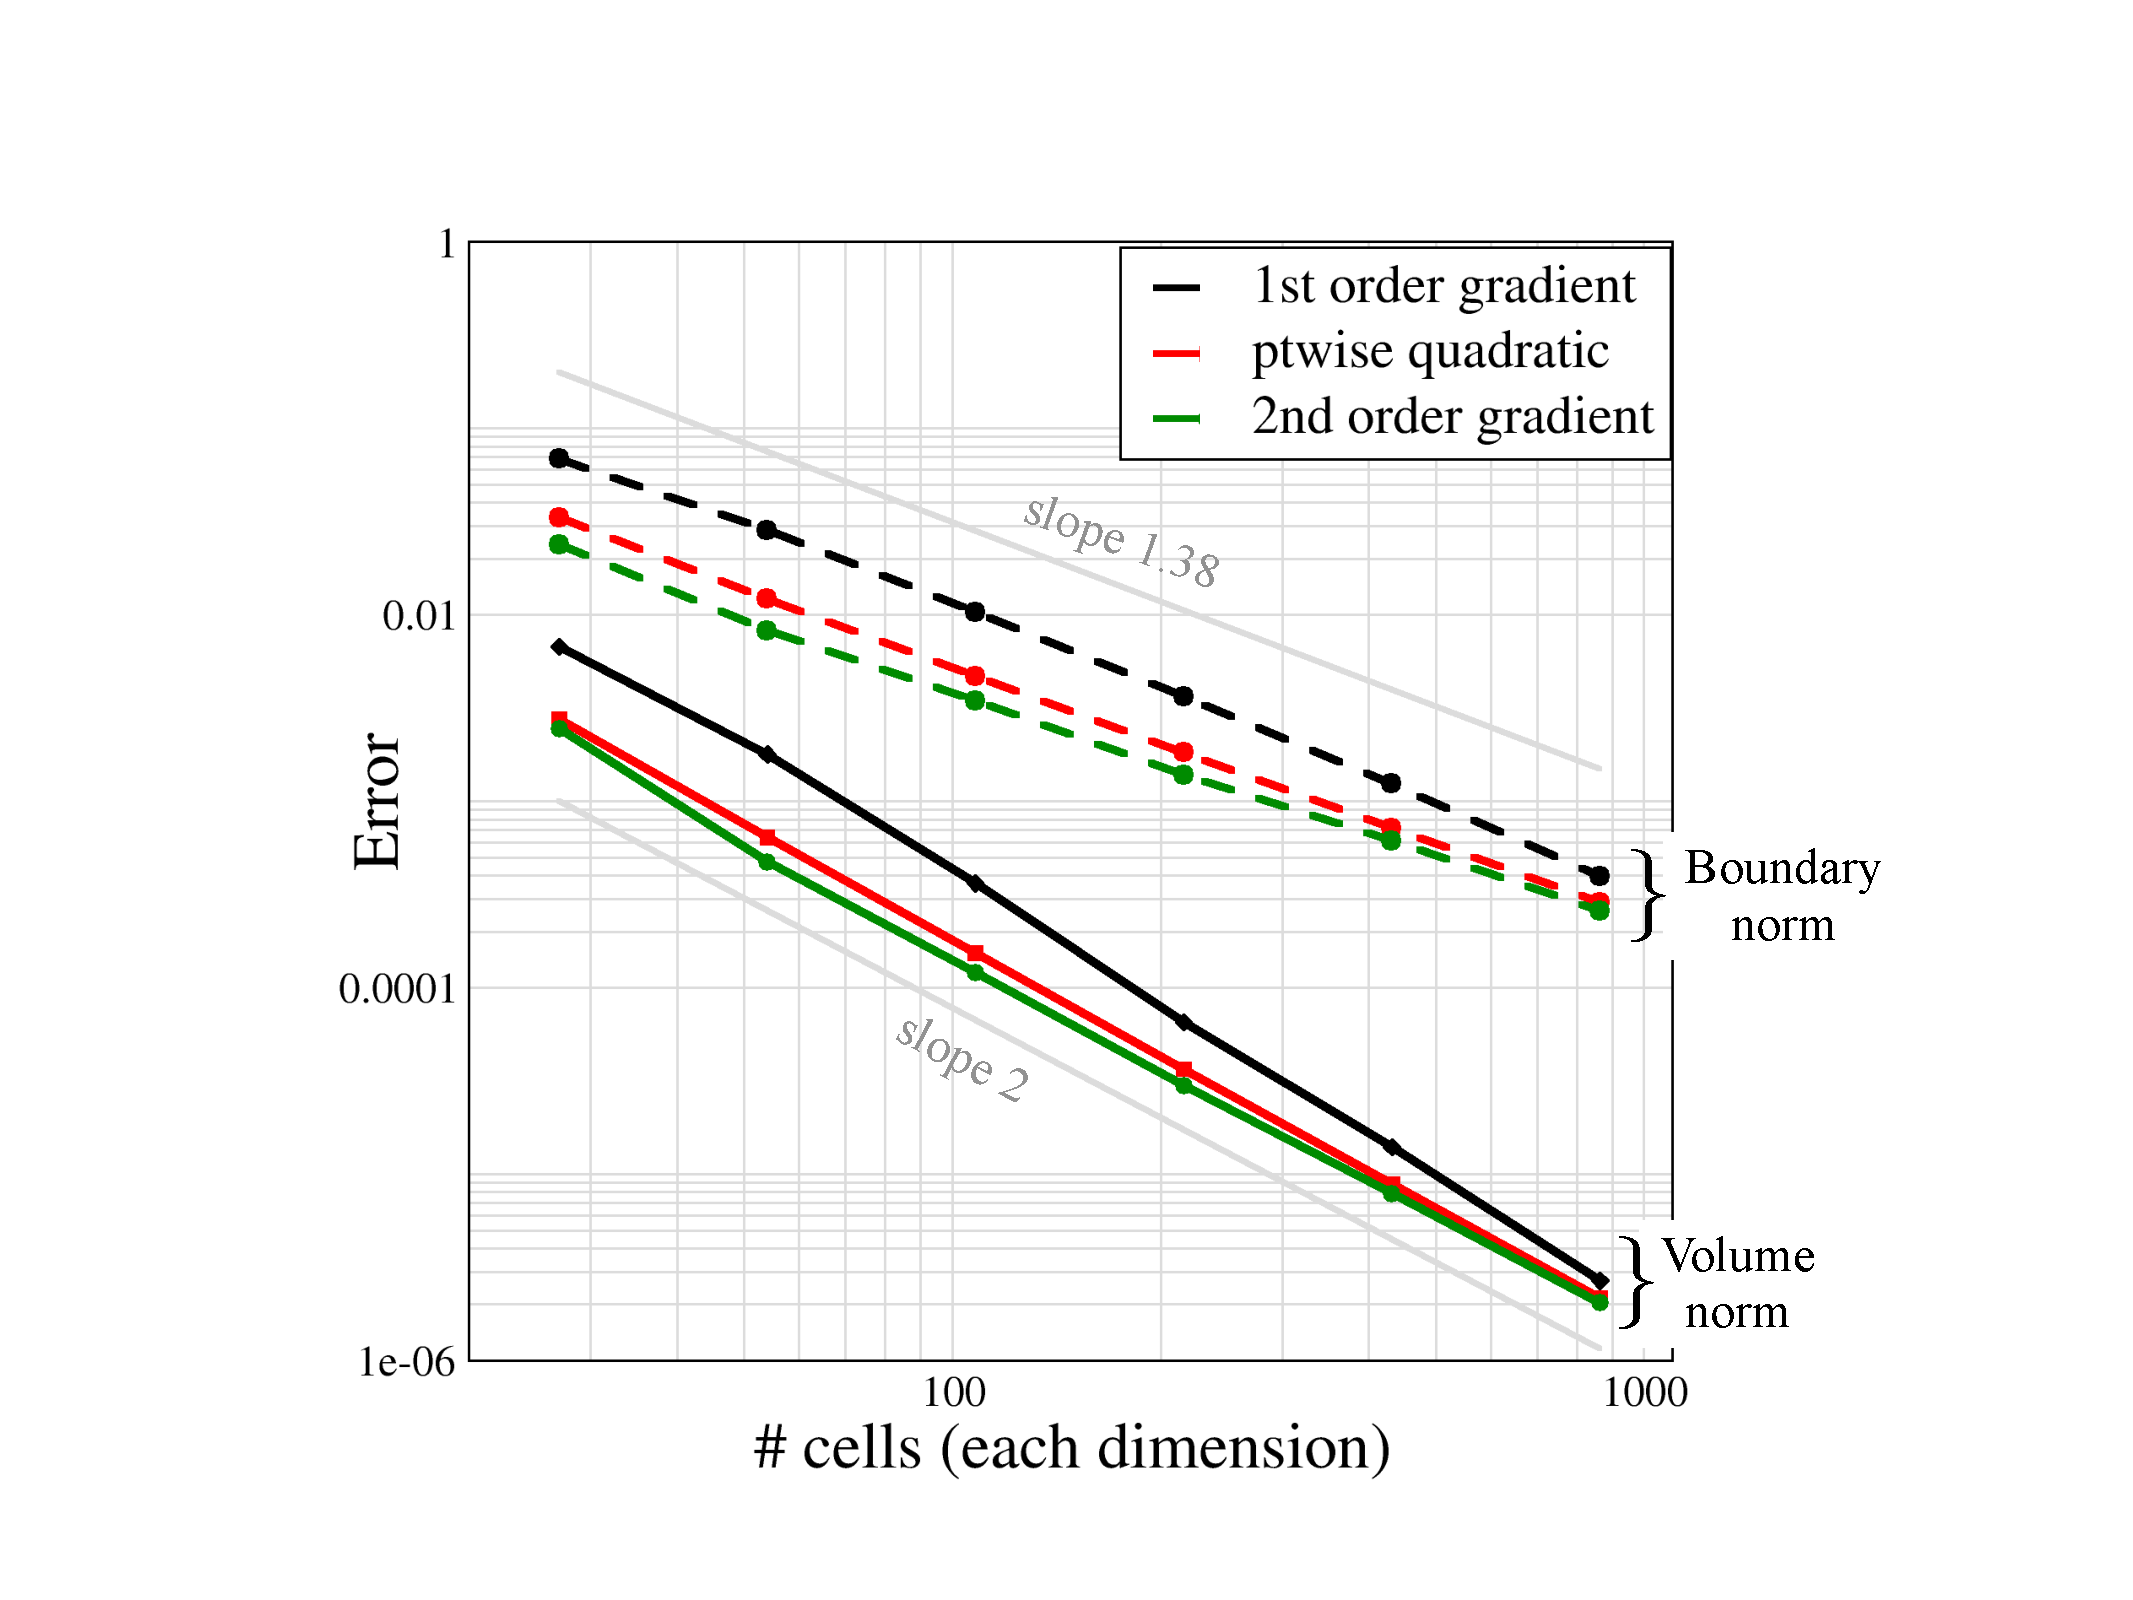
\includegraphics[height=3.0in]{figs/gradientConv.pdf}
		\caption{\sf Convergence in the L1 norm of the error in the entire 
			domain  (solid line), and along the boundary (dashed line).
			The reference line has slope 2 next to the domain error. The convergence
			rate at the boundary is between 1.38 and 1.5
			along the boundary.
			\label{fig:ssv}}
	\end{center}
\end{figure}


Note that the error at the cut cells is larger than in the volume, and has a
slower convergence rate. Since the number of cut cells grows only
linearly with refinement, the $L_1$
accuracy in the entire flow field is still second order.  At the boundary,
Richardson extrapolation shows that the convergence rate seems to be
between 1.38 and 1.5.
This has also been found in other cut cell studies \cite{KB:2006,nemec_tm14}, and 
is not due to SRD.

Figure \ref{fig:ssv} and Table \ref{tab:ssv}  show that using pointwise 
quadratic cut cell gradients is roughly
a factor of 2 more accurate on coarser grids.  The more complicated second order
acccurate gradient is even more accurate, especially on coarser grids.  Ultimately the gradient
error is reduced, and the error curves for the first and second order 
accurate gradients approach each other. 


We also use this example to compare the effect of state redistribution versus 
marching to steady state using local time-stepping without SRD.  
Table  \ref{tab:ssv2} shows a comparison of the error in the converged
solution using local time stepping (LTS)  without SRD, and the error with full timesteps and
SRD stabilization, both using  first order accurate gradients. 
The errors are essentially identical, showing that 
SRD does not degrade the computed solution with too much diffusion due
to the merging neighborhoods. This holds across all the other
gradient formulations too.


{
\small
\begin{table}[h]
\centering
 	\begin{tabular}{|l|c|l|l||l|l|} \hline
 		$h$ & $N_x ,N_y$ & \multicolumn{2}{|c|} {Volume Error} & \multicolumn{2}{|c|}{Boundary Error} \\ 
                \hline
 		    &            & {LTS (no SRD)} & SRD  & LTS (no SRD)  & SRD  \\ \hline
 			.5297 & 27 & 6.09e-3  &  6.75e-3   &  6.75e-02       &  6.84e-02 \\
 			\hline
 			.2648 & 54  & 1.67e-3  (3.6)  & 1.78e-4 (3.8)  &  2.79e-02  (2.4) &  2.83e-02 (2.4) \\
 			\hline
 			.1324 &108 & 3.41e-3  (4.9)  & 3.63e-4 (4.9)   &  1.00e-02  (2.8) &  1.03e-02  (2.8)\\
 			\hline
 			.662e-2 & 216 & 6.62e-5  (5.2)  & 6.52e-5 (5.6)  &  3.51e-03  (2.9) &  3.65e-03  (2.8)\\
 			\hline
 			.331e-2 & 432 & 1.34e-5  (4.9)  & 1.40e-5 (4.7)  &  1.21e-03  (2.9) &  1.24e-03  (3.0)  \\
 			\hline
 			.166e-2 & 864 & 2.59e-6  (5.2)  & 2.68e-6 (5.2)  &  3.78e-04  (3.2) &  3.96e-04  (3.1)  \\
 			\hline \hline
 	\end{tabular}
 	\caption{\sf Comparison of errors using local time stepping, which does not use SRD, 
        and regular time stepping with SRD. (The SRD errors are repeated here for easier
        comparison.) The errors are almost identical, except on the coarsest
        grid, showing that SRD does not 
        degrade the solution with too much diffusion. \label{tab:ssv2}}
\end{table}
}



\subsection{Shock Reflection from  Cylinder}
Next we demonstrate the method for the Euler equations using a Mach 2
shock diffracting around a circular cylinder. A cylinder with radius $0.15$ is centered at
(0.5,0.5), and the shock is initially located at $x = 0.2$.
For this example we compare results using the MUSCL scheme and
the Method of Lines as the base schemes, both using local Lax Friedrichs for the Riemann
solver. The BJ limiter is used to limit
both the base scheme irregular cells  and tile reconstruction gradients. 

Figure \ref{fig:cyl1} (left) shows the solution density from MUSCL, and
right from MOL, at time $t=0.25$. 
Both grids use 302 cells in each
directions, and the domain is  $[0.0,0.0,]$ by  $[1.00001, 1.0]$, again to
prevent mesh degeneracies.
There are 416 cut cells
around the cylinder; 160 of the cut cells had volume fractions less than
0.5 and were stabilized with SRD.  The smallest volume fraction was 1.17E-4.   
For comparison, this is also the time shown in \cite{mjb-hel-rjl:hbox2}. 
Here and in \cite{mjb-hel-rjl:hbox2}, the front of the cylinder where the
maximum density is found is better behaved with the one-step methods than with
MOL.  The method of lines solution is smoother around the boundary than our
MUSCL variant (see Figure \ref{fig:cylbndry}).

\begin{figure}[h]
\begin{center}
\vspace*{-.1in}
\hspace*{-.4in}
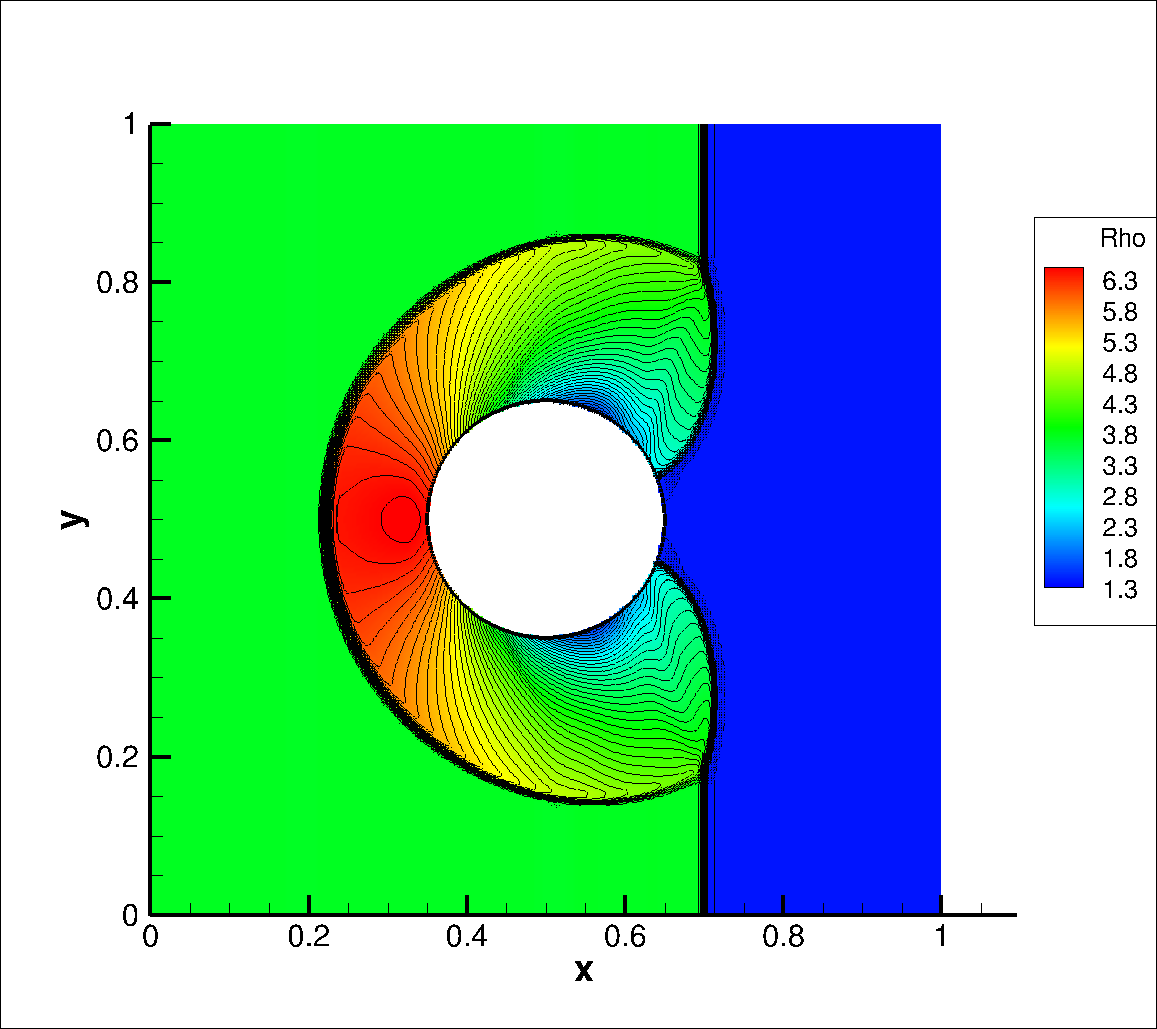
\includegraphics[width=0.48\linewidth,trim=10 10 200 10,clip]{figs/muscl_302cells.png}
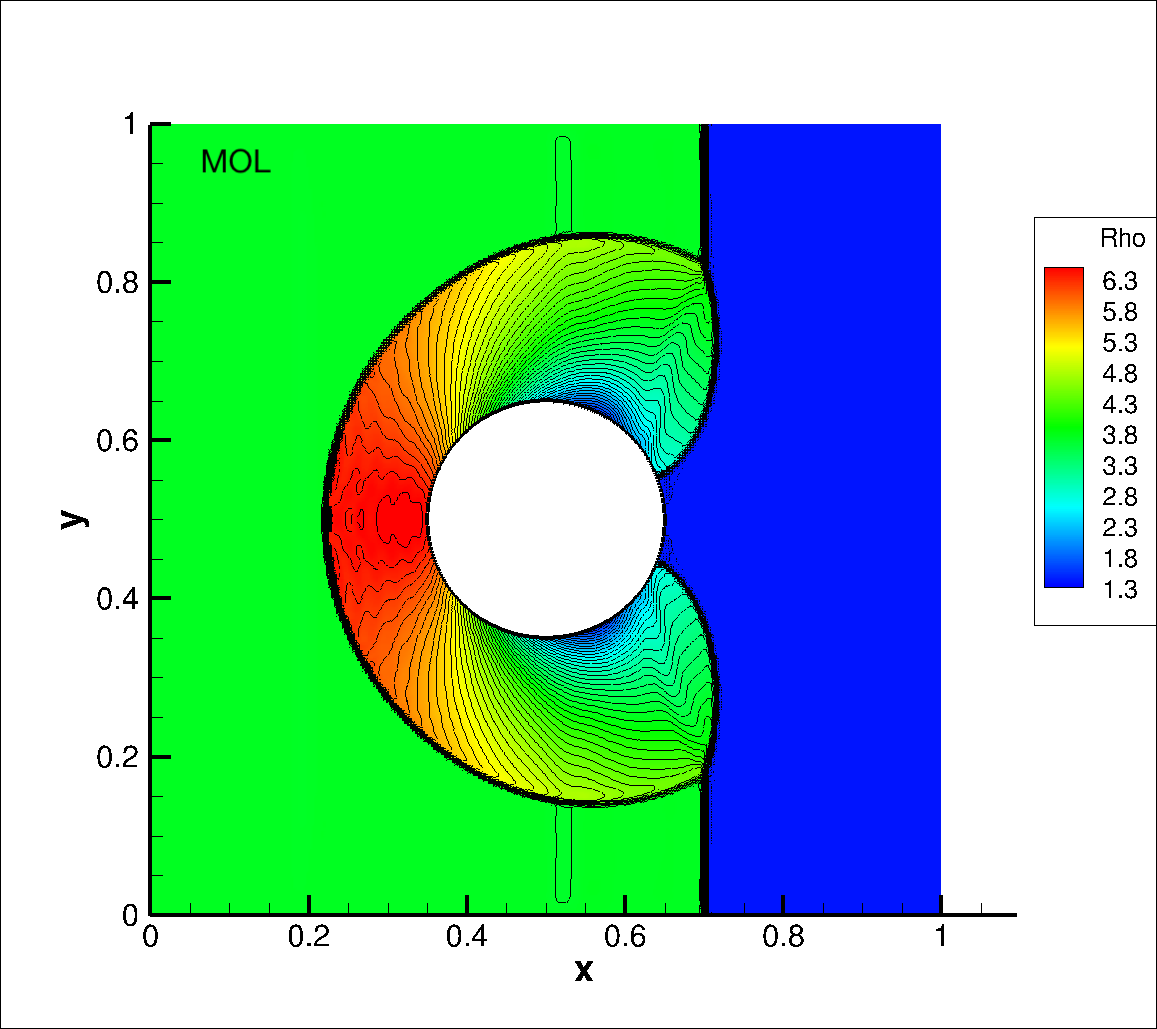
\includegraphics[width=0.48\linewidth,trim=10 10 200 10,clip]{figs/MOL_302cells.png}
\caption{\sf Density profile of Mach 2 shock reflection around a cylinder,
at time t=0.25.  Left computation used MUSCL, right used MOL. 
There are 52 contours between 1.3 and 6.5.
The front of the cylinder is better behaved with MUSCL, but the solution
at the cut cells is better  with the method of lines.
\label{fig:cyl1}}
\end{center}
\vspace*{-.1in}
\end{figure}

Figure \ref{fig:cylbndry}
shows the density profile from both schemes
taken along the cylinder.
For this plot, the cut cell variable is
reconstructed to the midpoint of the cylinder line segment in each  cell.  
The zoom shows the difference more
clearly.

\begin{figure}
\begin{center}
%\includegraphics[width=0.48\linewidth,trim=20 20 20 30,clip]{figs/densityCompare_302_normalvs3by3.png}
\hspace*{-.5in}
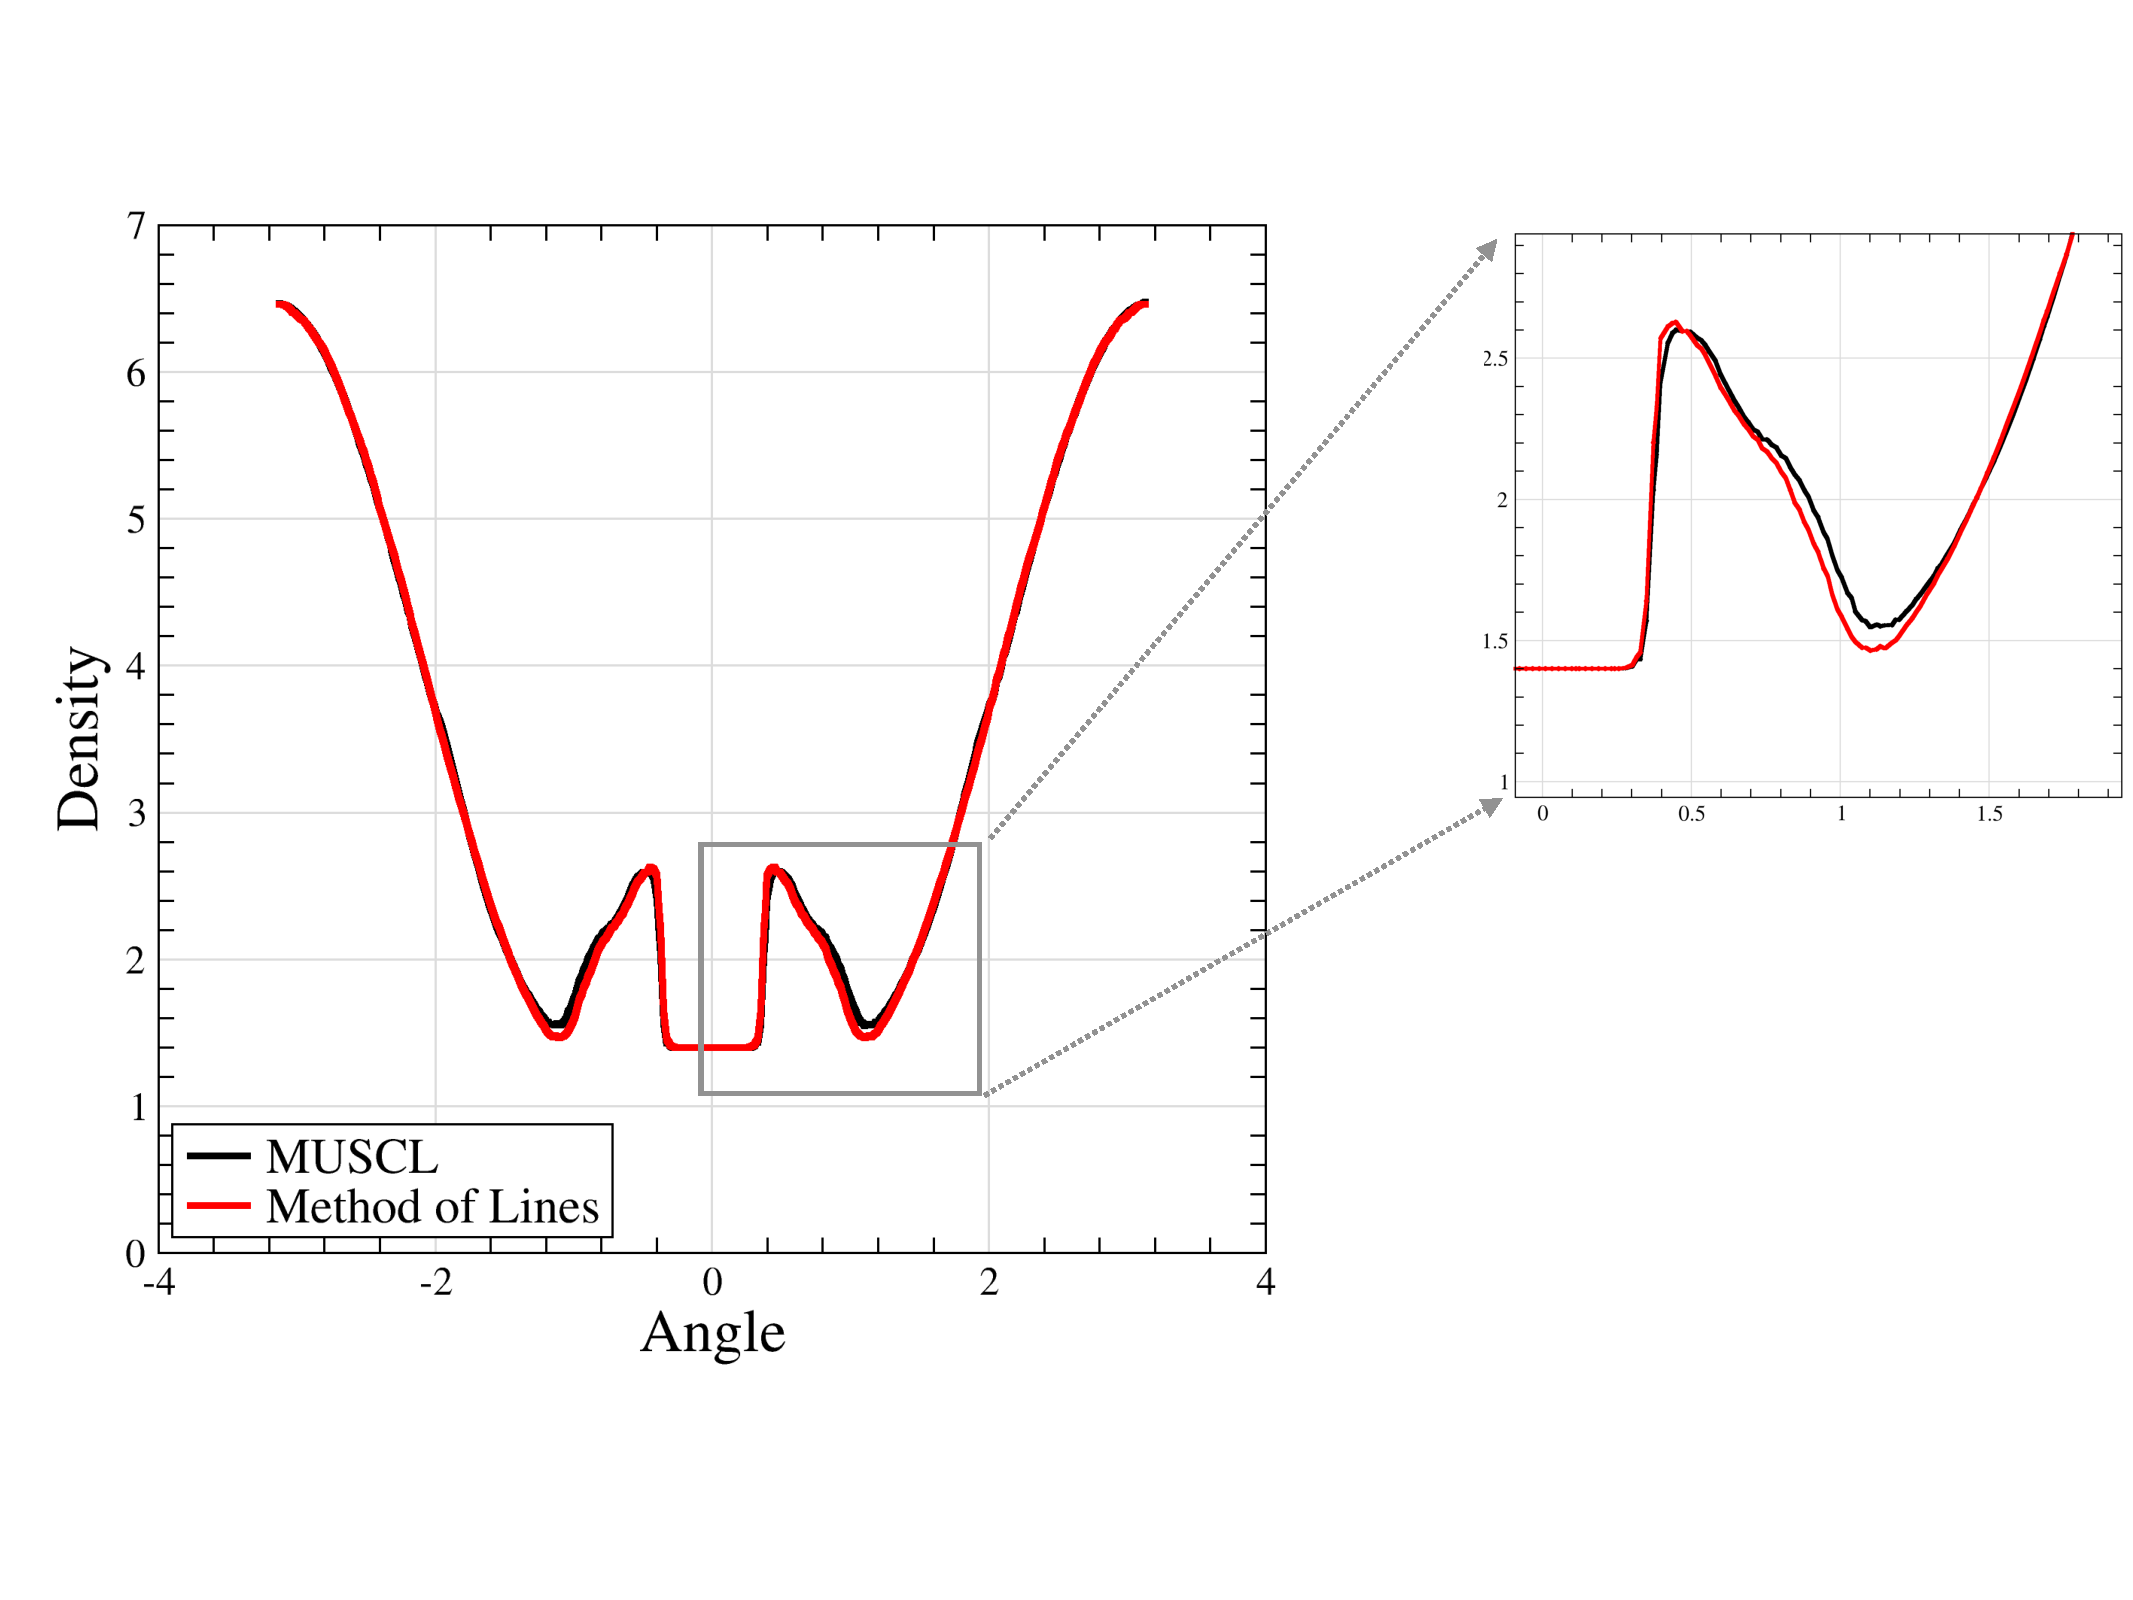
\includegraphics[height=2.7in]{figs/MM_densityBndry.pdf}
\hspace*{.3in}
%\includegraphics[width=0.48\linewidth,trim=20 20 20 30,clip]{figs/pressureCompare_302_normalvs3by3.png}
%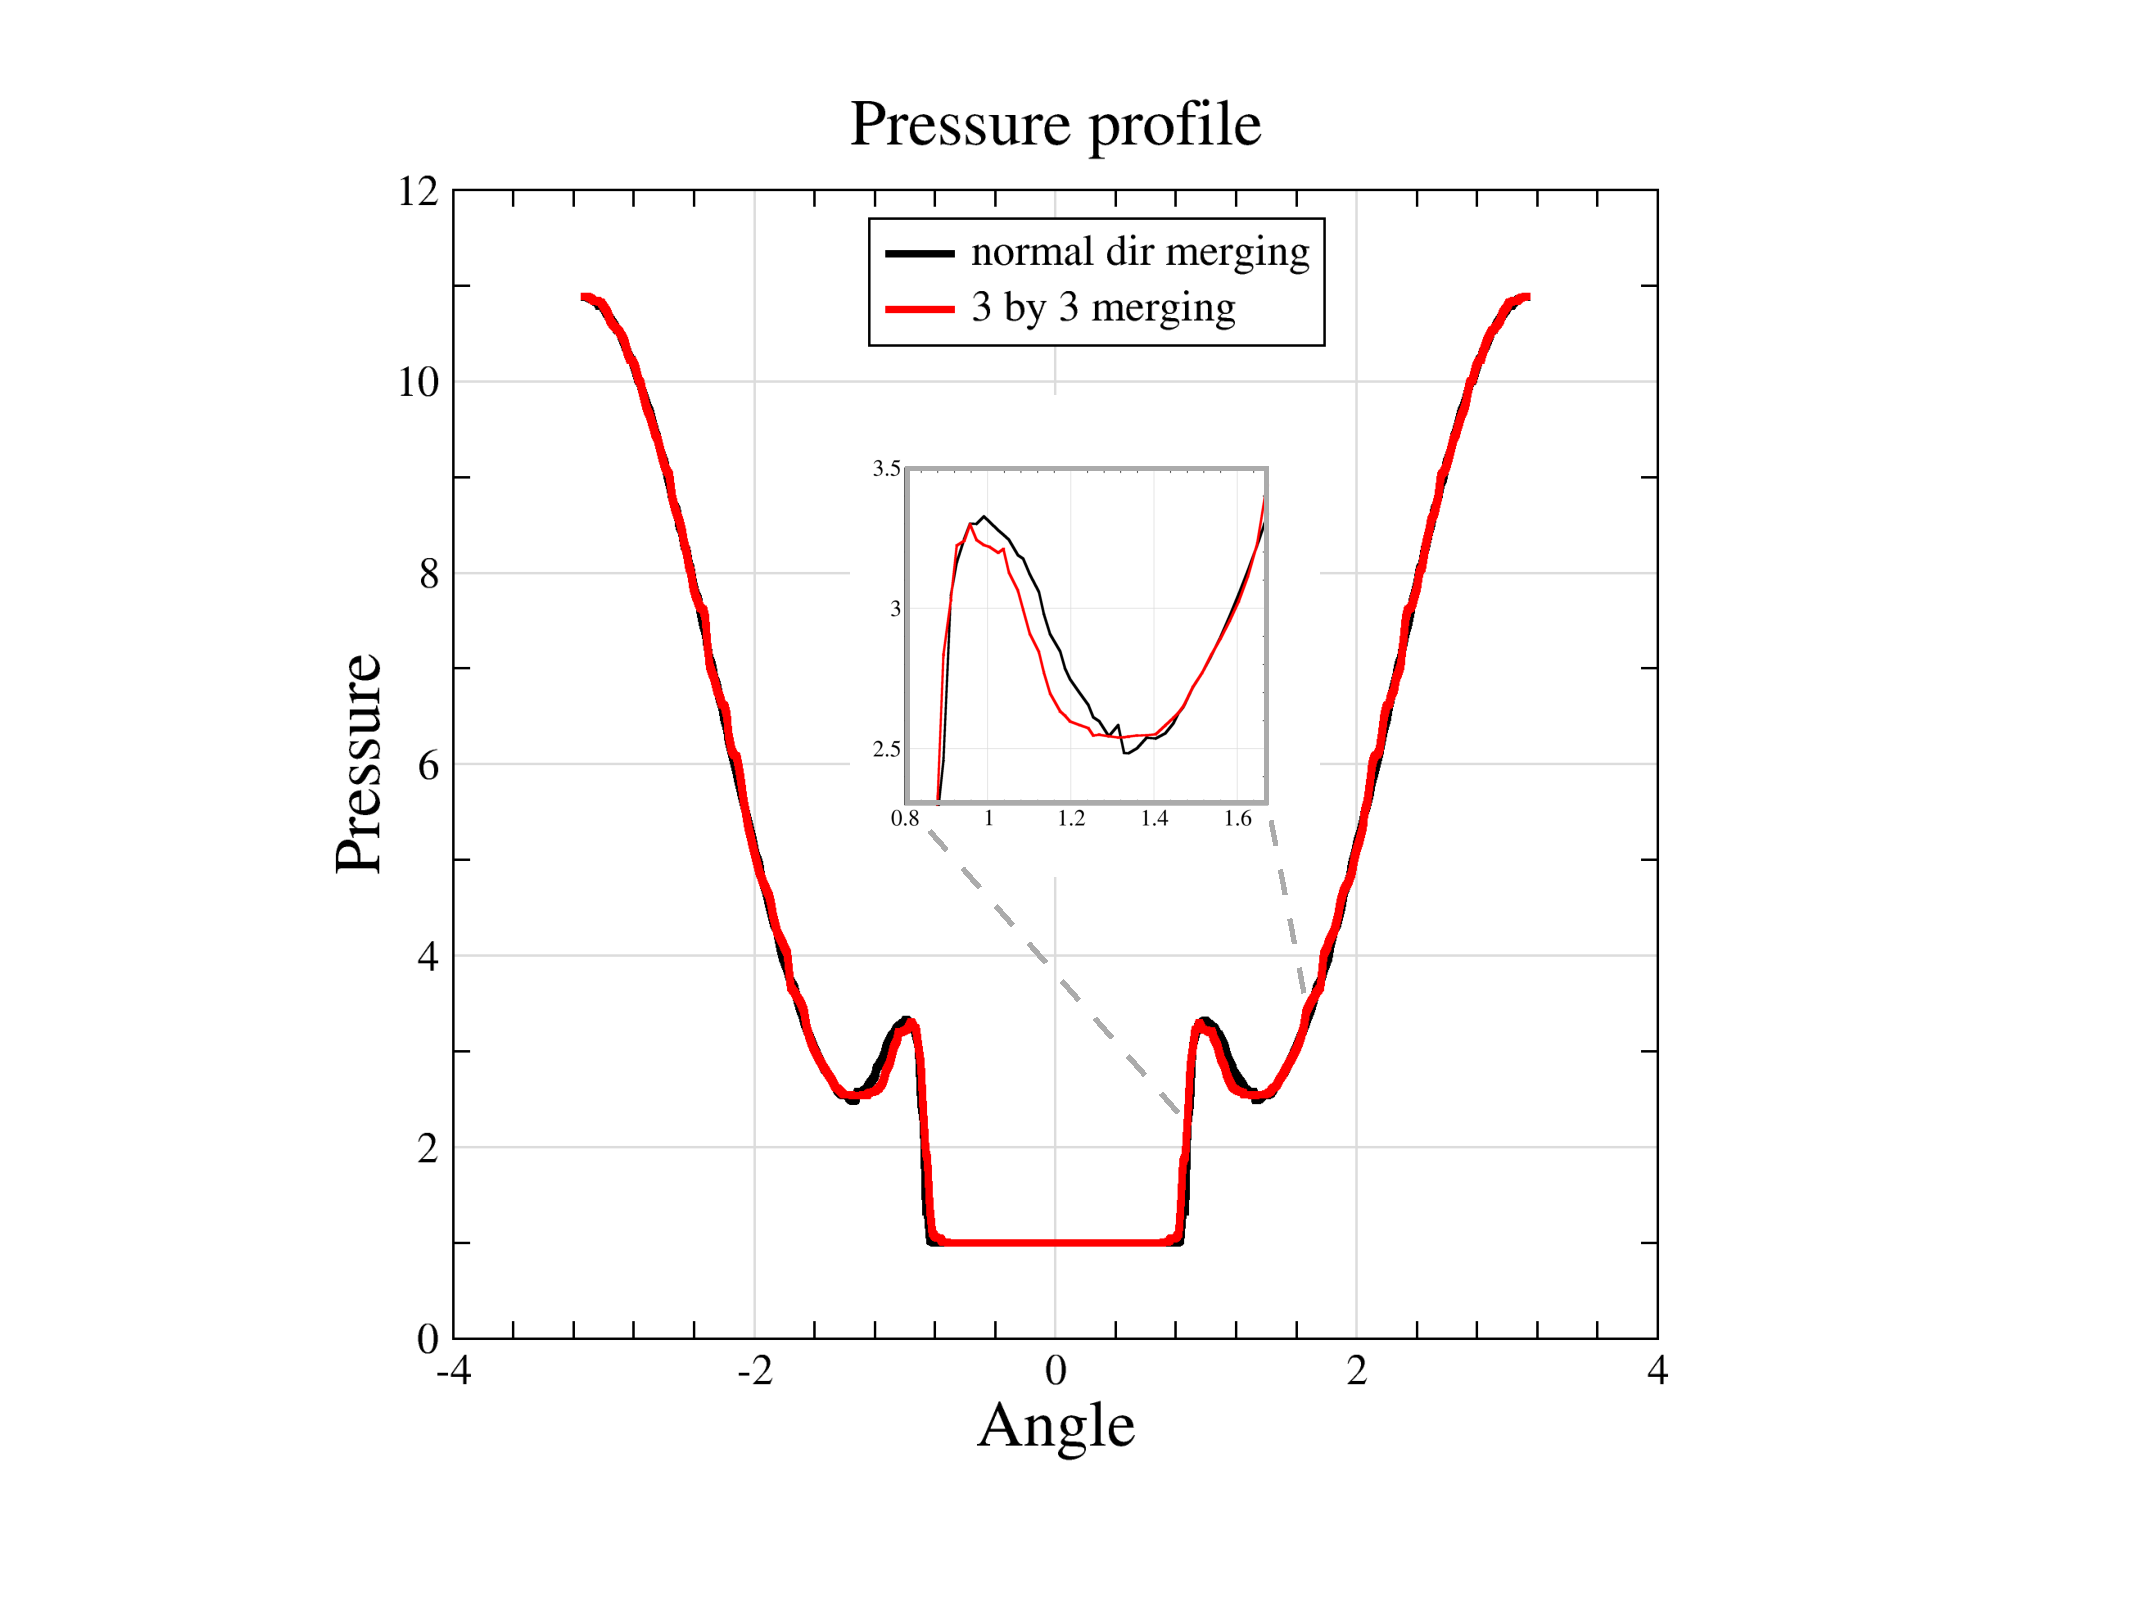
\includegraphics[height=2.7in,trim=120 70 230 50,clip]{figs/pressureWithZoom.pdf}
\caption{\sf The density profile  around the cylinder for the MUSCL and MOL schemes 
at time t=0.25.  The MOL scheme has smoother results.}
\label{fig:cylbndry}
\end{center}
% fig in amrclaw-amrcart/example/cylinder_Mach2 directory on juniper
% using sortedcyl.dat (coied from bndry01.dat) in the various _output dirs
\end{figure}

\clearpage

\subsection{Double Mach Reflection problem}\label{sec:dm}
In this section, we reflect a Mach 10 shock obliquely over a wedge, 
where the shock and wall form a $60^{\circ}$ angle.  
The problem domain is $[0,3.0]\times[0,1.75]$, with an angled wall 
passing through the point $(1/6,0)$ . The ramp is outlined in red in Figure
\ref{fig:dm}.
We use the finite volume MUSCL scheme with second order slopes on the base 
grid and SRD neighborhoods, and limit using Barth Jespersen.
The solution to this problem is a complex, self-similar reflection pattern 
composed of incident and reflected shocks, Mach stem, and a contact 
discontinuity \cite{WOODWARD1984115,rkdg5}.  
The contact discontinuity is an unstable feature of the solution that can be 
difficult to resolve correctly, especially in the neighborhood of the 
reflecting boundary where the carbuncle phenomenon can occur \cite{KEMM2018596}.

\begin{figure}[h]
\centering
%\includegraphics[width=0.48\linewidth]{figs/doublemach.png}
%\includegraphics[width=0.48\linewidth]{figs/doublemach_zoom.png}
%\includegraphics[width=1.1\linewidth]{figs/doubleMach.pdf}
\hspace*{-.25in}
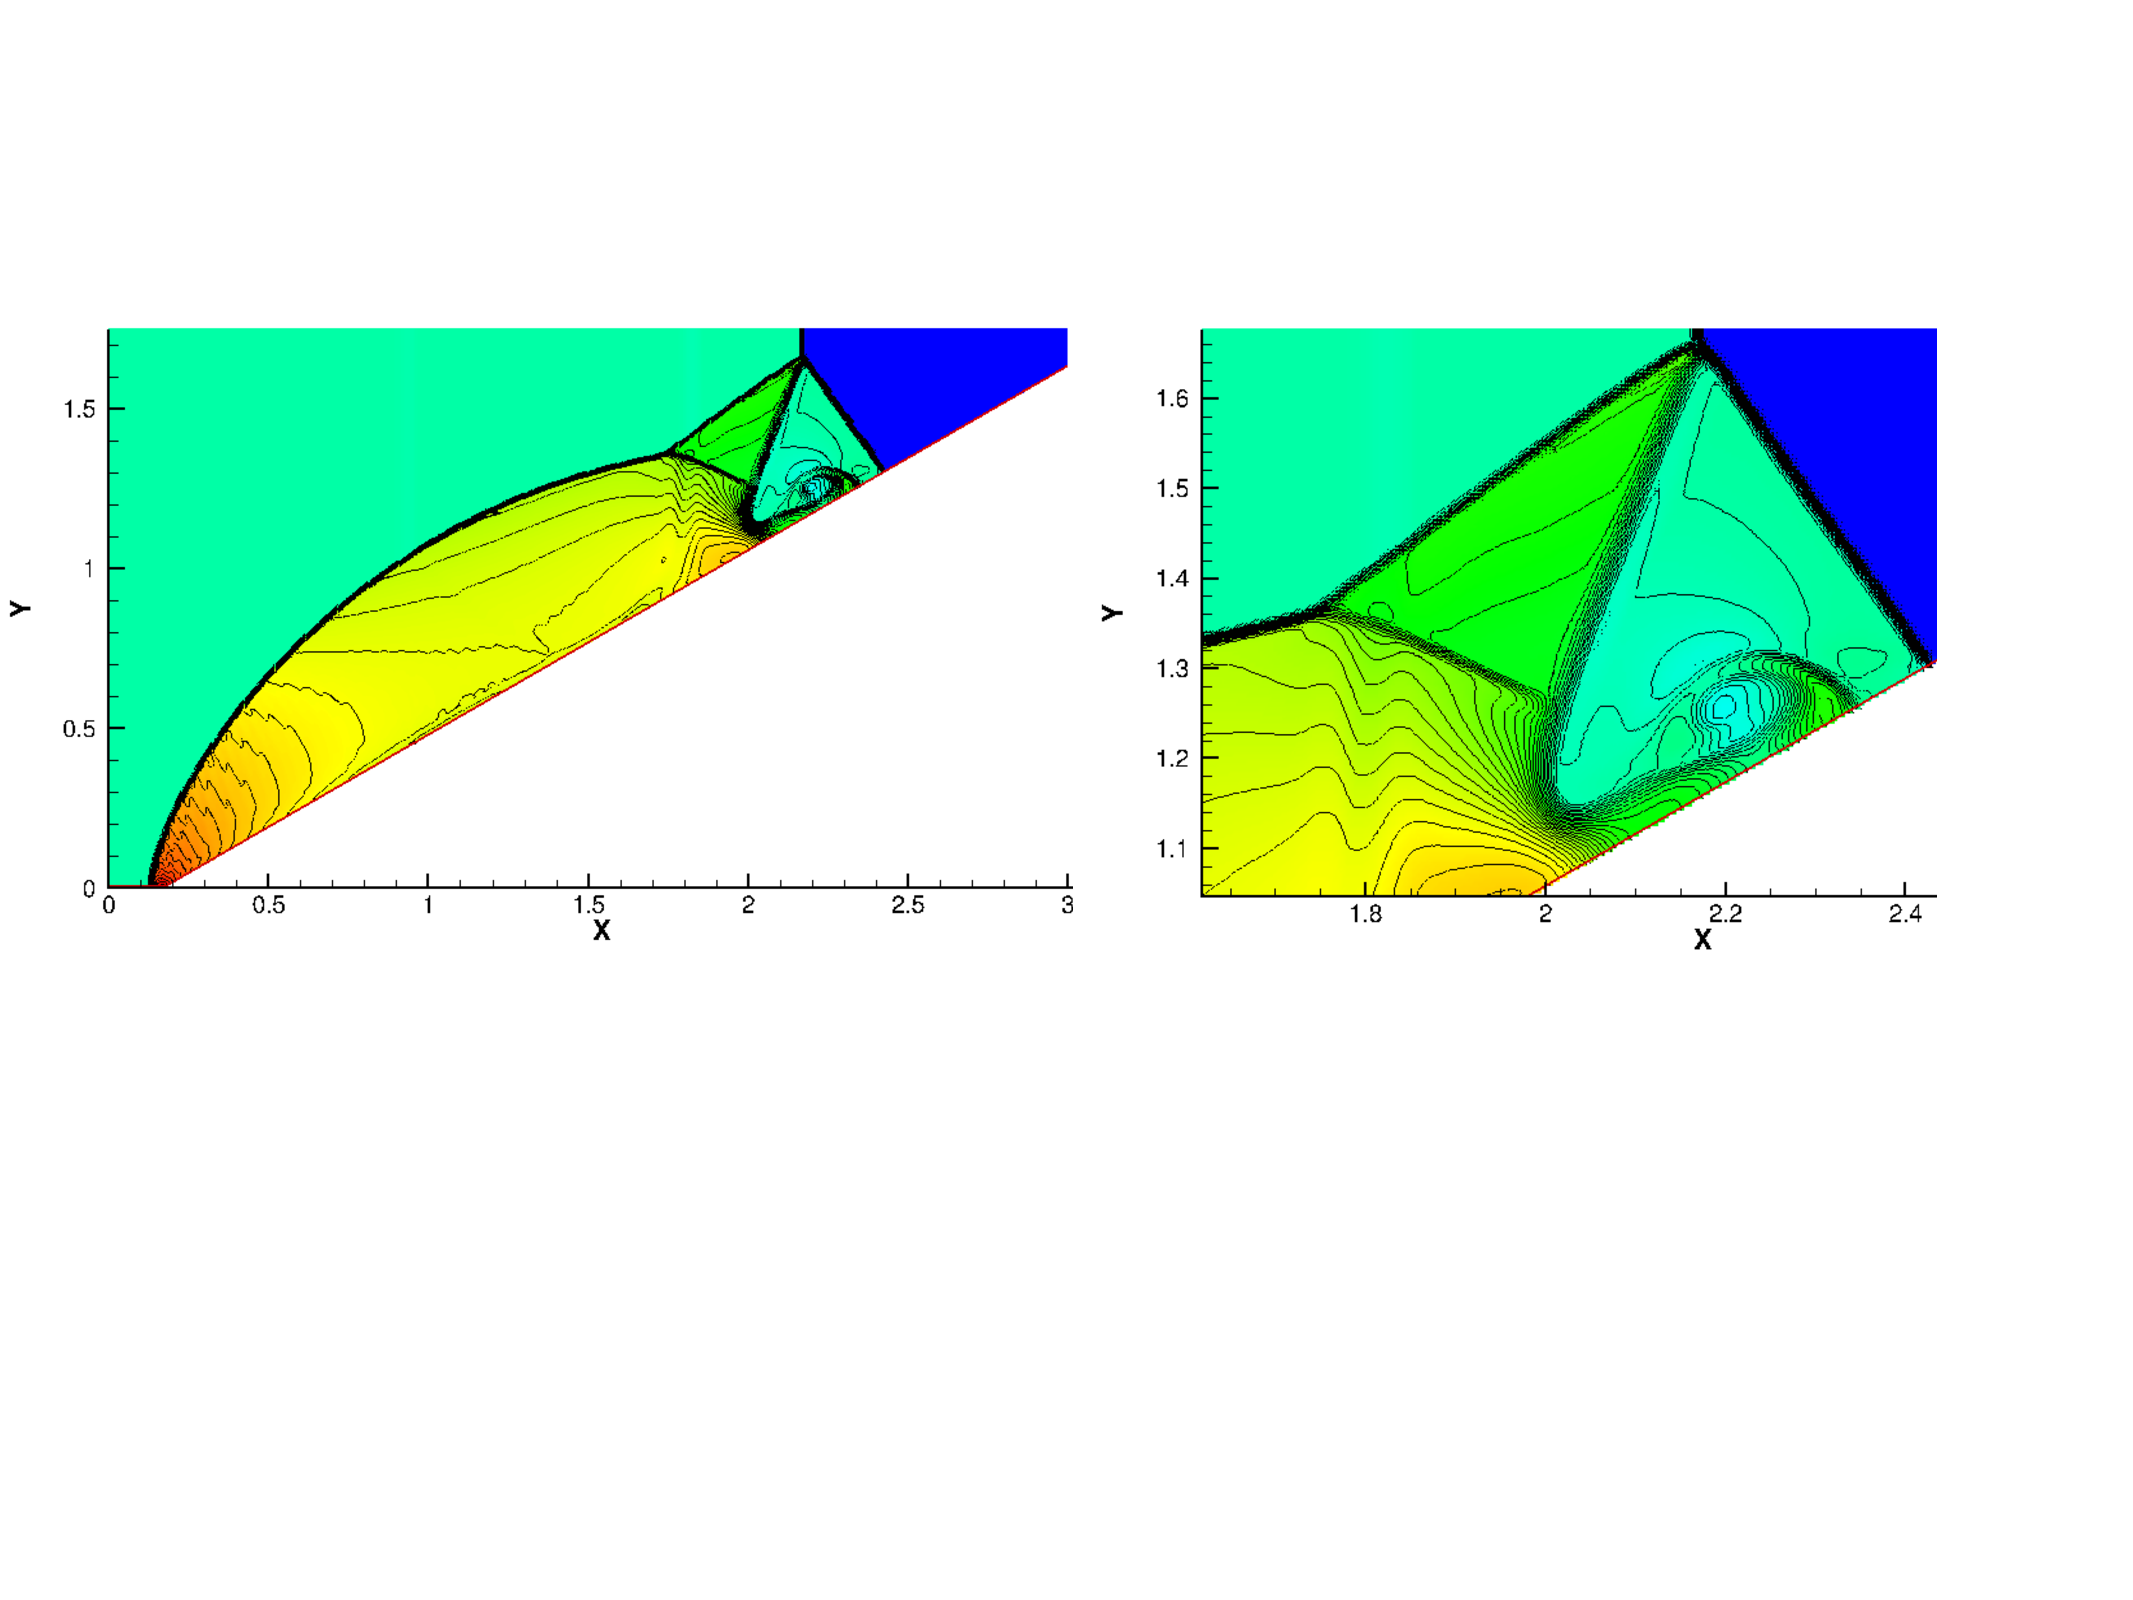
\includegraphics[width=1.1\linewidth]{figs/doubleMach240.pdf}
\hspace*{-.25in}
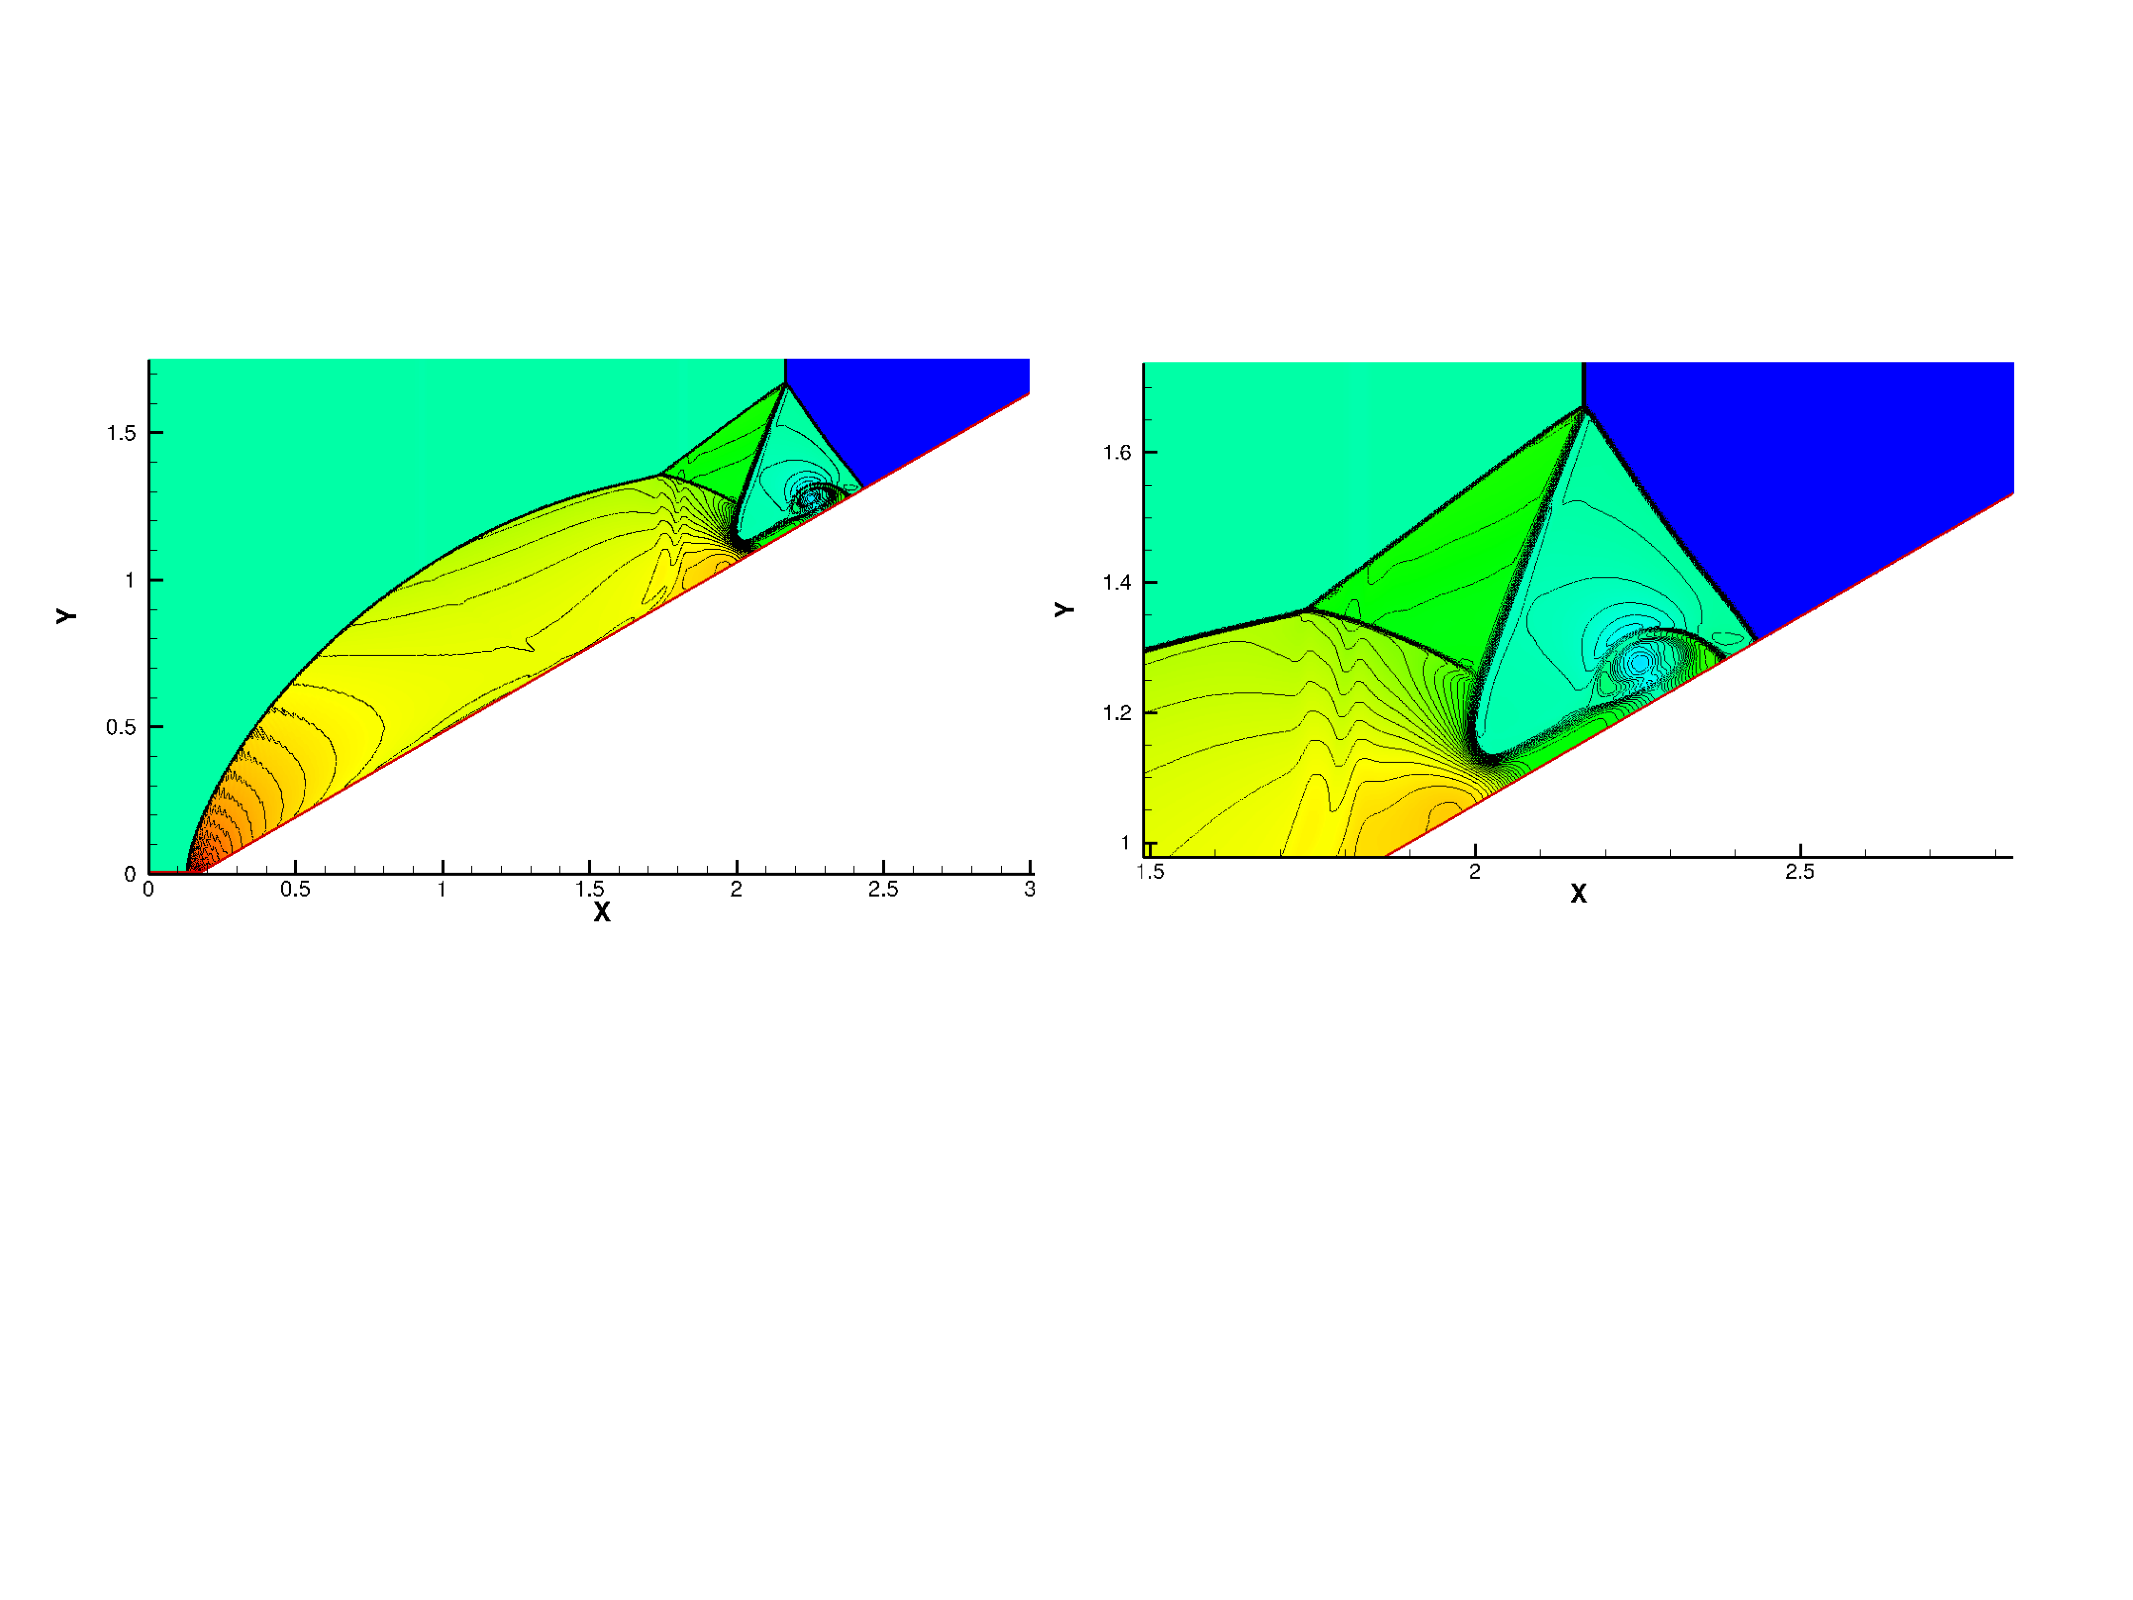
\includegraphics[width=1.1\linewidth]{figs/doubleMach480.pdf}
\caption{\sf Density plot and isolines of a Mach 10 shock impinging 
obliquely on a wedge at time $t = 0.2$ where $\Delta x = \Delta y =
1/240$ (top) and 1/480 (bottom).
The solution on the full domain is shown adjacent to a zoom of the Mach 
stem region.  Sixty isolines between 1.39 and 21.0 are drawn.}\label{fig:dm}
\end{figure}

The solution at the final time $T = 0.2$ is plotted in Figure \ref{fig:dm}, 
where the grid resolution is $\Delta x = \Delta y = 1/240$.
We obtain qualitatively comparable results to those in \cite{rkdg5} on 
the same grid resolution. We also show for comparison the results using 
$\Delta x = \Delta y = 1/480$, also done in \cite{rkdg5}. Again, the
improvement is very similar. Finally, in Figure \ref{fig:wedgeBndry} we
show the density along the boundary for the two resolutions. Despite the
irregularity of the cut cells, the solution is very smooth. The smallest
cut cell in the coarser grid has volume fraction 1.65e-6. On the finest
grid the smallest volume fraction is 2.95e-7. 

\begin{figure}[h]
\centering
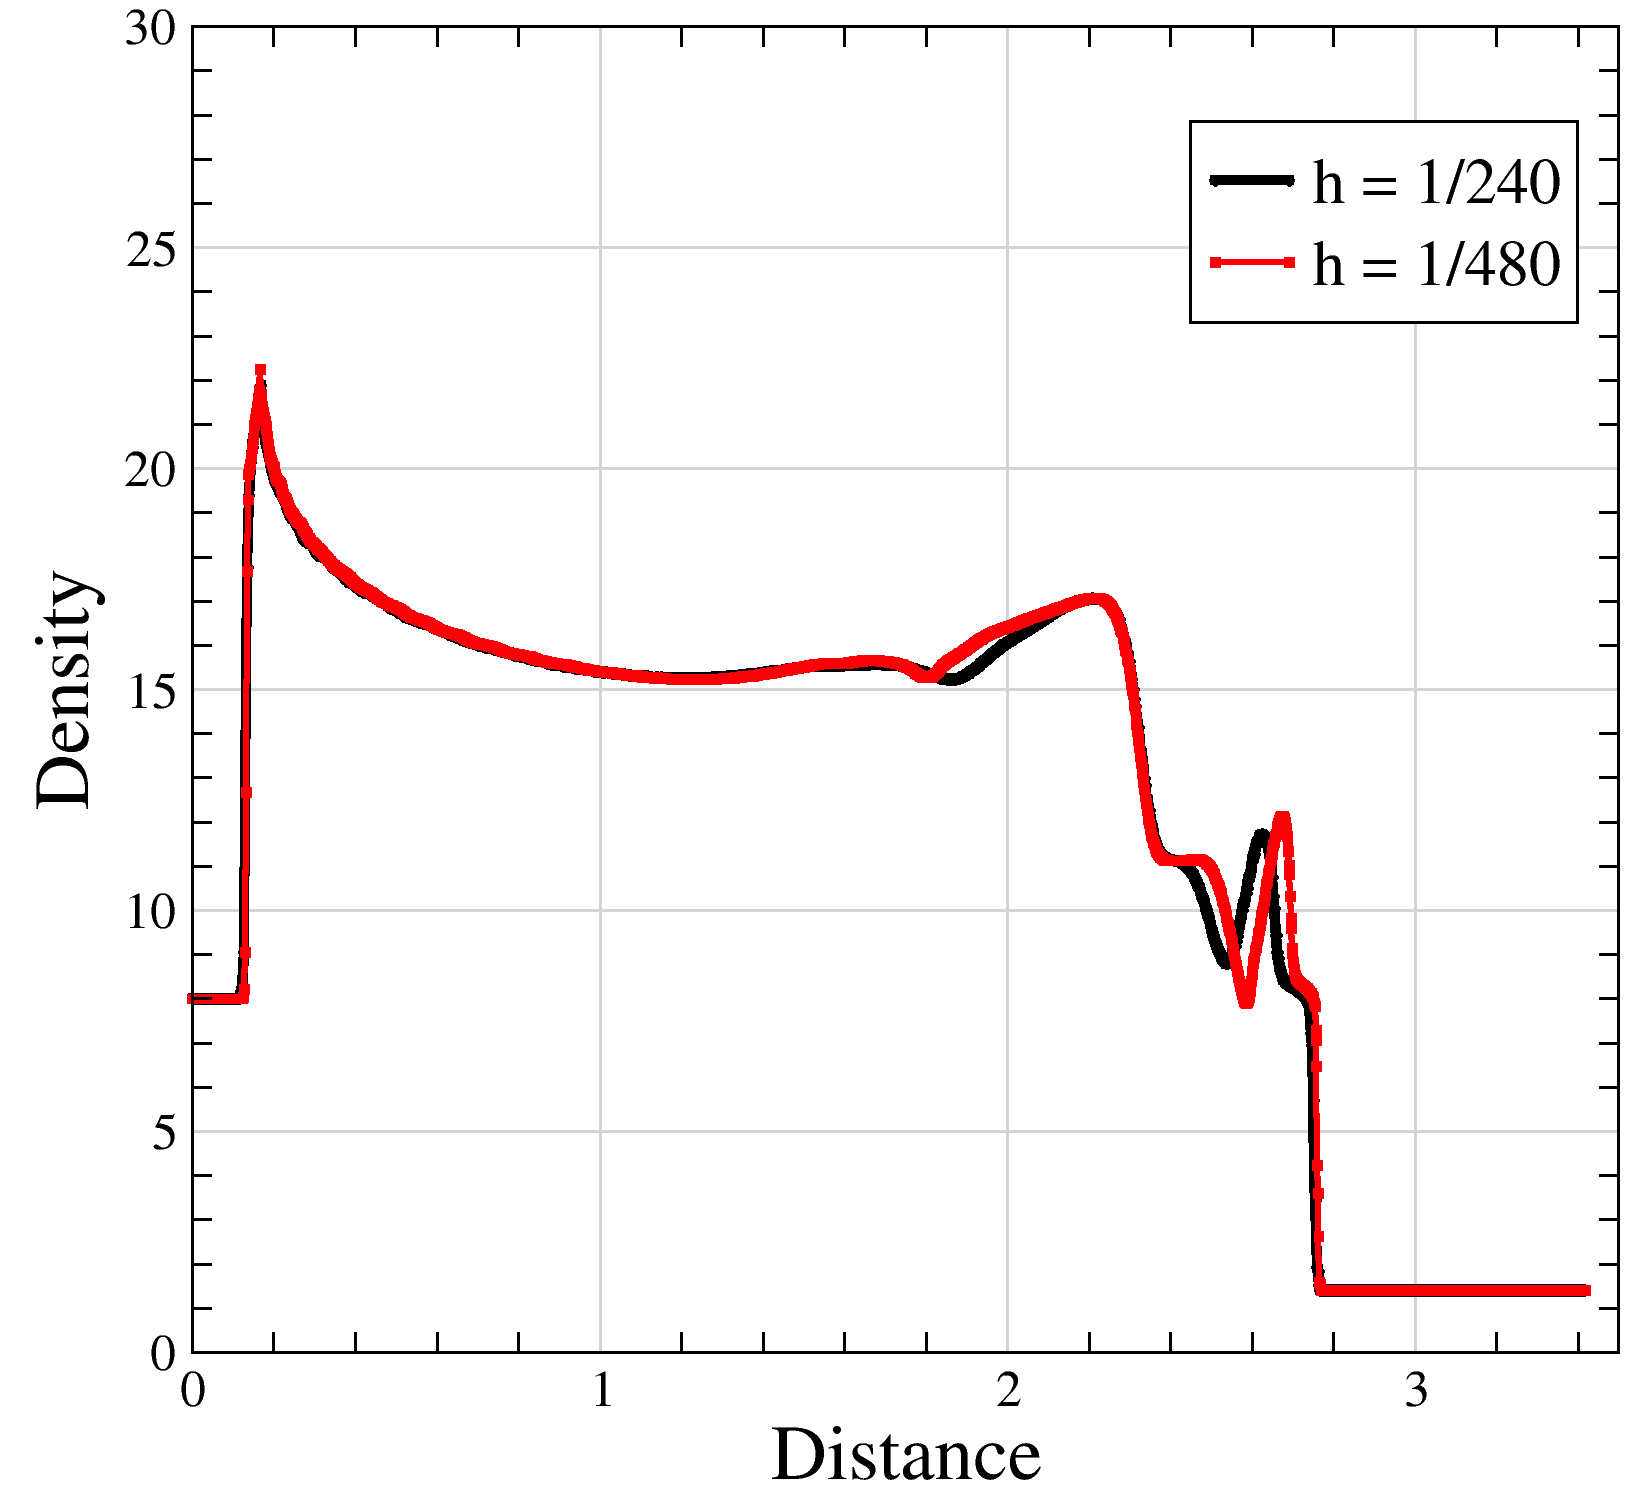
\includegraphics[width=.7\linewidth]{figs/rampWall.png}
\caption{\sf Density plotted along the wall, as a function of distance from
the lower left corner of the domain. The coarser grid has a bit of
oscillation after the ramp starts due to the curved shock. It is not due to
SRD. It is not present on the finer grid .} \label{fig:wedgeBndry}
\end{figure}




\section{Conclusions}\label{sec:conc}
We have presented a  state redistribution algorithm to solve the small cell problem on cut cell meshes.  It is conservative, allows for overlapping temporary merging neighborhoods so is easy to implement, and is linearity preserving.   
Numerical experiments show that on smooth problems, second order accuracy is maintained, and the solution is not degraded by the postprocessing. For problems with shocks, the scheme maintains robustness at the cut cells.
We have shown experiments using SRD on two different base schemes, but it should be 
applicable to any underlying numerical method with
cell-centered variables.

We think that state redistribution should be applicable to 
different sets of equations, and to three-dimensional applications.
It also seems clear that the scheme can be extended to higher order accuracy, 
when used in conjunction with a 
higher order base scheme. We have already started extending this work to
3rd and 4th order accuracy. Higher order methods bring 
in many new features however, so we do not include that here.




%\subsection*{Acknowledgments} 



\bibliography{/Users/berger/references}
\bibliographystyle{plain}



\end{document}
